% Informe del repositorio wcd-nacl-crns-simulations: analysis/replica-Sidelnik-MEIGA_seccion-4.1.1
% Contenido identico a la Sec. 4.1.1 de la tesis (fuente comun: seccion_4_1_1.tex y apendice_procesos.tex);
% scripts/construir_informe.py genera cuerpo_informe.tex y apendice_informe.tex con la jerarquia de titulos del informe.
\documentclass[11pt,letterpaper]{article}
\usepackage[utf8]{inputenc}
\usepackage[T1]{fontenc}
\usepackage[spanish]{babel}
\decimalpoint
\usepackage{lmodern}
\usepackage{amsmath,amssymb}
\usepackage[left=3cm,right=3cm,top=2.5cm,bottom=2.5cm,headheight=14pt]{geometry}
\usepackage{graphicx}
\usepackage{float}
\usepackage{booktabs}
\usepackage{multirow}
\usepackage{tabularx}
\usepackage{longtable}
\usepackage{makecell}
\usepackage{array}
\usepackage{adjustbox}
\usepackage{changepage}
\usepackage{pdflscape}
\usepackage{afterpage}
\usepackage{rotating}
\usepackage[table]{xcolor}
\usepackage{caption}
\usepackage{subcaption}
\captionsetup{font=small,labelfont=bf}
\usepackage{siunitx}
\sisetup{output-decimal-marker={.}}
\usepackage{enumitem}
\usepackage[backend=biber,style=authoryear,natbib=true,maxcitenames=2,maxbibnames=99,uniquename=false,uniquelist=false]{biblatex}
\addbibresource{bibliografia-1.bib}
\DeclareDelimFormat{multicitedelim}{\addsemicolon\space}
\usepackage{fancyhdr}
\usepackage{titlesec}
\definecolor{colortitulo}{RGB}{0,70,140}
\usepackage[colorlinks=true,linkcolor=colortitulo,citecolor={rgb:red,140;green,72;blue,20},urlcolor=colortitulo]{hyperref}
\addto\captionsspanish{\renewcommand{\tablename}{Tabla}\renewcommand{\listtablename}{Índice de tablas}}
\setlength{\parskip}{0.25cm}
\setlength{\parindent}{0pt}
\setlength{\emergencystretch}{3em}
\renewcommand{\topfraction}{0.9}\renewcommand{\bottomfraction}{0.8}\renewcommand{\textfraction}{0.07}\renewcommand{\floatpagefraction}{0.75}
\titleformat{\section}{\normalfont\Large\bfseries\color{colortitulo}}{\thesection}{0.8em}{}
\titleformat{\subsection}{\normalfont\large\bfseries\color{colortitulo}}{\thesubsection}{0.8em}{}
\titleformat{\paragraph}[runin]{\normalfont\normalsize\bfseries}{}{0em}{}
\numberwithin{equation}{section}
\numberwithin{figure}{section}
\numberwithin{table}{section}
\graphicspath{{Figuras/}{../figuras/}}
\pagestyle{fancy}\fancyhf{}
\fancyhead[L]{\small\textcolor{colortitulo}{Réplica de Sidelnik et al.\ (2020) con MEIGA: neutrones de 500~MeV}}
\fancyhead[R]{\small\textcolor{colortitulo}{\thepage}}
\fancyfoot[C]{\footnotesize\textcolor{gray}{wcd-nacl-crns-simulations · analysis/replica-Sidelnik-MEIGA\_seccion-4.1.1}}
\renewcommand{\headrulewidth}{0.5pt}

\begin{document}
\thispagestyle{empty}
\begin{center}
{\small\textcolor{gray}{Informe técnico del repositorio \texttt{wcd-nacl-crns-simulations} · \texttt{analysis/replica-Sidelnik-MEIGA\_seccion-4.1.1}}}\\[1.2cm]
{\LARGE\bfseries\textcolor{colortitulo}{Validación numérica del modelo Monte Carlo de un detector Cherenkov de agua dopada con NaCl:\\[0.2cm] réplica con MEIGA de la simulación de Sidelnik et al.\ (2020) con neutrones de 500~MeV}}\\[1.0cm]
{\large Jaime A. Betancourt}\\[0.2cm]
{Doctorado en Ciencias Naturales -- Física, Universidad Industrial de Santander}\\[0.2cm]
{19 de octubre de 2026}
\end{center}
\vspace{0.6cm}
\begin{abstract}
\noindent Se reprodujeron con el simulador MEIGA (\textsc{Geant4} 10.7.p04, \texttt{QGSP\_BERT\_HP\_NoThermal}, sin $S(\alpha,\beta)$) la geometría, los materiales y la irradiación del detector Cherenkov de agua dopada con NaCl de \citet{Sidelnik2020}, con $1.5\times10^{5}$ neutrones de 500~MeV en agua pura y en agua con 2.5, 5 y 10\,\% de NaCl. La validación sigue la cadena física completa: interacción del neutrón primario, moderación, captura, gammas de captura, electrones secundarios, luz Cherenkov y carga en el PMT. El modelo reproduce la moderación ($\xi_{\mathrm{H}}=1.000$, $\xi_{\mathrm{O}}=0.118$), la probabilidad de captura (24.08\,\% frente a 25.18\,\% en agua pura), el tiempo de captura y su reducción con la sal (de 192 a 75~µs), las líneas $\gamma$ de captura, el espectro de electrones en escala absoluta (dentro del 4--8\,\%) y la distribución de fotones Cherenkov aceptados entre 0 y 500 fotones sin reescalar; las curvas de razón NaCl/agua pura coinciden en forma con las del artículo ($r=0.88$--$0.91$). Las diferencias se atribuyen a la mayor producción de piones del modelo de Bertini, a un fondo de desexcitación nuclear mayor, a un aumento de la captura con la sal más débil y al modelo de captura de \textsc{Geant4}, que no conserva la energía en las cascadas del Cl. Este informe reproduce, con la misma redacción, figuras y tablas, la Sec.~4.1.1 de la tesis doctoral del autor.
\end{abstract}
\vspace{0.3cm}
\tableofcontents
\clearpage

% ARCHIVO GENERADO por scripts/construir_informe.py a partir de seccion_4_1_1.tex: no editar aqui.
%==========================================================================
% PROPUESTA DE NUEVA SECCIÓN 4.1.1 (reemplaza a la Sec. 4.1.1 de cap4_resultados.tex)
% Basada en las corridas MEIGA de octubre de 2026 (150 000 neutrones de 500 MeV por medio)
% y en el informe del repositorio analysis/replica-Sidelnik-MEIGA_seccion-4.1.1/.
% Figuras: ../figuras/ (análisis) y Figuras/ (figuras de Sidelnik et al. 2020 ya usadas en la tesis).
% Incluye los cuatro medios: agua pura y agua + 2.5, 5 y 10 % NaCl.
%==========================================================================
\section{Introducción y configuración de la simulación}
\label{sec:Res-WCD-500MeV}

\noindent Con el propósito de evaluar y validar el modelo Monte Carlo desarrollado en este trabajo, se reprodujeron las principales condiciones geométricas, físicas y de irradiación del detector Cherenkov de agua dopada con NaCl descrito por \citet[Sec.~2, pp.~2217--2218, Fig.~1]{Sidelnik2020}.\footnote{Los resultados de este informe se obtuvieron con corridas del simulador MEIGA, con $1.5\times10^{5}$ neutrones de 500~MeV por medio, la misma geometría y la misma física en todos los medios. El análisis completo, los programas y los datos reducidos se encuentran en el repositorio del proyecto \citep{Betancourt2026WCDNaCl}, carpeta \texttt{analysis/replica-Sidelnik-MEIGA\_seccion-4.1.1}. Se simularon los cuatro medios: \textcolor{red}{agua pura}, \textcolor{green}{agua + 2.5 \% de NaCl}, \textcolor{violet}{agua + 5 \% de NaCl} y \textcolor{orange}{agua + 10 \% de NaCl}.} La estrategia de validación se realizó de manera progresiva, siguiendo la cadena de procesos físicos que conduce desde la interacción inicial del neutrón con el medio detector hasta la generación de la señal óptica: la interacción del neutrón primario de alta energía, la moderación de los neutrones secundarios mediante dispersiones elásticas, su captura, la emisión de fotones gamma de captura $\gamma_{\mathrm{Cap}}$, la producción de electrones y positrones secundarios y, finalmente, la generación de radiación Cherenkov y la respuesta del tubo fotomultiplicador.

Los principales parámetros geométricos, físicos y de simulación adoptados para realizar esta comparación se resumen en la Tabla~(\ref{par-simula}). En ella se identifican tanto las condiciones reproducidas directamente del modelo de referencia como aquellas implementadas específicamente en el presente trabajo.

\begin{table}[!tp]
	\centering
	\captionsetup{width=\linewidth,justification=justified,singlelinecheck=false}
	\caption[Parámetros empleados en la validación del modelo WCD.]{Parámetros geométricos, materiales y de simulación del modelo \textsc{Geant4} (MEIGA) desarrollado en este trabajo, frente a la configuración del detector WCD de \citet{Sidelnik2020}. La última columna indica dónde se encuentra cada dato en dicho trabajo.}
	\label{par-simula}
	\footnotesize
	\renewcommand{\arraystretch}{1.12}
	\setlength{\tabcolsep}{4pt}
	\newcommand{\grupo}[1]{\rowcolor{gray!15}\multicolumn{4}{c}{\textbf{#1}} \\}
	\begin{tabularx}{\linewidth}{>{\raggedright\arraybackslash}p{0.25\linewidth} >{\raggedright\arraybackslash}X >{\raggedright\arraybackslash}X >{\raggedright\arraybackslash}p{0.15\linewidth}}
		\toprule
		\textbf{Parámetro} & \textbf{Este trabajo} & \textbf{Sidelnik et al. (2020)} & \textbf{Referencia} \\
		\midrule
		\grupo{Geometría del detector}
		Altura / diámetro del tanque & 133 cm / 96 cm & 133 cm / 96 cm & Sec.~2, p.~2217 \\
		Radio del tanque & 48 cm & 48 cm$^{a}$ & Sec.~2, p.~2217 \\
		Volumen activo & $\approx 1~\mathrm{m^{3}}$ & $\approx 1~\mathrm{m^{3}}$ & Sec.~1, p.~2217 \\
		Tanque & Acero inoxidable de 0.5 mm (lados, tapa y fondo) & Acero inoxidable de 0.5 mm & Sec.~2, p.~2217 \\
		\grupo{Revestimiento interno}
		Material y espesor & Tyvek, 0.12 mm & Tyvek, $\approx$\,0.12 mm & Sec.~2, p.~2217 \\
		Modelo óptico & Reflector difuso (\texttt{groundbackpainted}) con la reflectividad medida del Tyvek$^{b}$ & Propiedades reflectivas y refractivas del Tyvek & Sec.~2, pp.~2217--2218 \\
		\grupo{Tubo fotomultiplicador}
		Modelo & Hamamatsu R5912, 8 pulgadas & Hamamatsu R5912, 8 pulgadas & Sec.~2, p.~2217 \\
		Superficie sensible & Sección esférica: radio 10.16 cm, altura 5 cm & Sección esférica: radio 10.16 cm, altura 5 cm & Sec.~2, p.~2217 \\
		Posición & Centro de la tapa superior & Centro de la tapa superior & Sec.~2; Fig.~1 \\
		\grupo{Fuente de neutrones y simulación}
		Partícula primaria & Neutrones de 500 MeV & Neutrones de 500 MeV & Sec.~2, p.~2218 \\
		Fuente & Haz horizontal a media altura (66.562 cm), 1 cm fuera de la pared & Haz horizontal sobre la pared lateral & Sec.~2; Fig.~1 \\
		Neutrones por medio & $1.5\times10^{5}$ & $1.5\times10^{5}$ & Sec.~2, p.~2218 \\
		Versión de \textsc{Geant4} & 10.7.p04 & No especificada & -- \\
		Lista física & QGSP\_BERT\_HP\_\allowbreak NoThermal, sin $S(\alpha,\beta)$; G4NDL~4.6 & No especificada & -- \\
		Detección de la luz & Eficiencia cuántica del R5912 aplicada al crearse cada fotón (modo \texttt{eFast}) & Eficiencia cuántica del PMT & Sec.~3, Fig.~6 \\
		\grupo{Medio detector}
		Configuraciones & \textcolor{red}{Agua pura}; \textcolor{green}{agua + 2.5\,\% NaCl}; \textcolor{violet}{agua + 5\,\% NaCl}; \textcolor{orange}{agua + 10\,\% NaCl} & Las mismas cuatro & Sec.~2, p.~2218 \\
		\bottomrule
	\end{tabularx}
	\vspace{0.1cm}
	\begin{minipage}{\linewidth}
		\footnotesize \textit{Notas:} $^{a}$Derivado del diámetro reportado ($D=96$ cm). $^{b}$Implementación propia de este trabajo; no reproduce un modelo de superficie óptica especificado por Sidelnik et al. Las corridas no incluyen la dispersión térmica $S(\alpha,\beta)$ (modelo de gas libre para los neutrones térmicos), como en la primera campaña de simulación.
	\end{minipage}
\end{table}

La Figura~(\ref{fig:esquema-evento}) muestra un evento real de la simulación sobre la geometría del detector. El neutrón de 500~MeV ingresa a media altura y sufre una interacción inelástica; los neutrones secundarios se moderan y algunos de ellos son capturados. Las capturas emiten fotones gamma cuyos electrones secundarios, de pocos milímetros de recorrido, generan la luz Cherenkov que finalmente alcanza el PMT. Cada eslabón de esta cadena se compara a continuación con el trabajo de referencia, cuyos resultados se presentan en la Sec.~3 (pp.~2218--2221) \citep[Sec.~3, pp.~2218--2221]{Sidelnik2020}.

\begin{figure}[!htbp]
	\begin{adjustwidth}{0cm}{0cm}
		\centering
		\begin{minipage}{\linewidth}
			\centering
			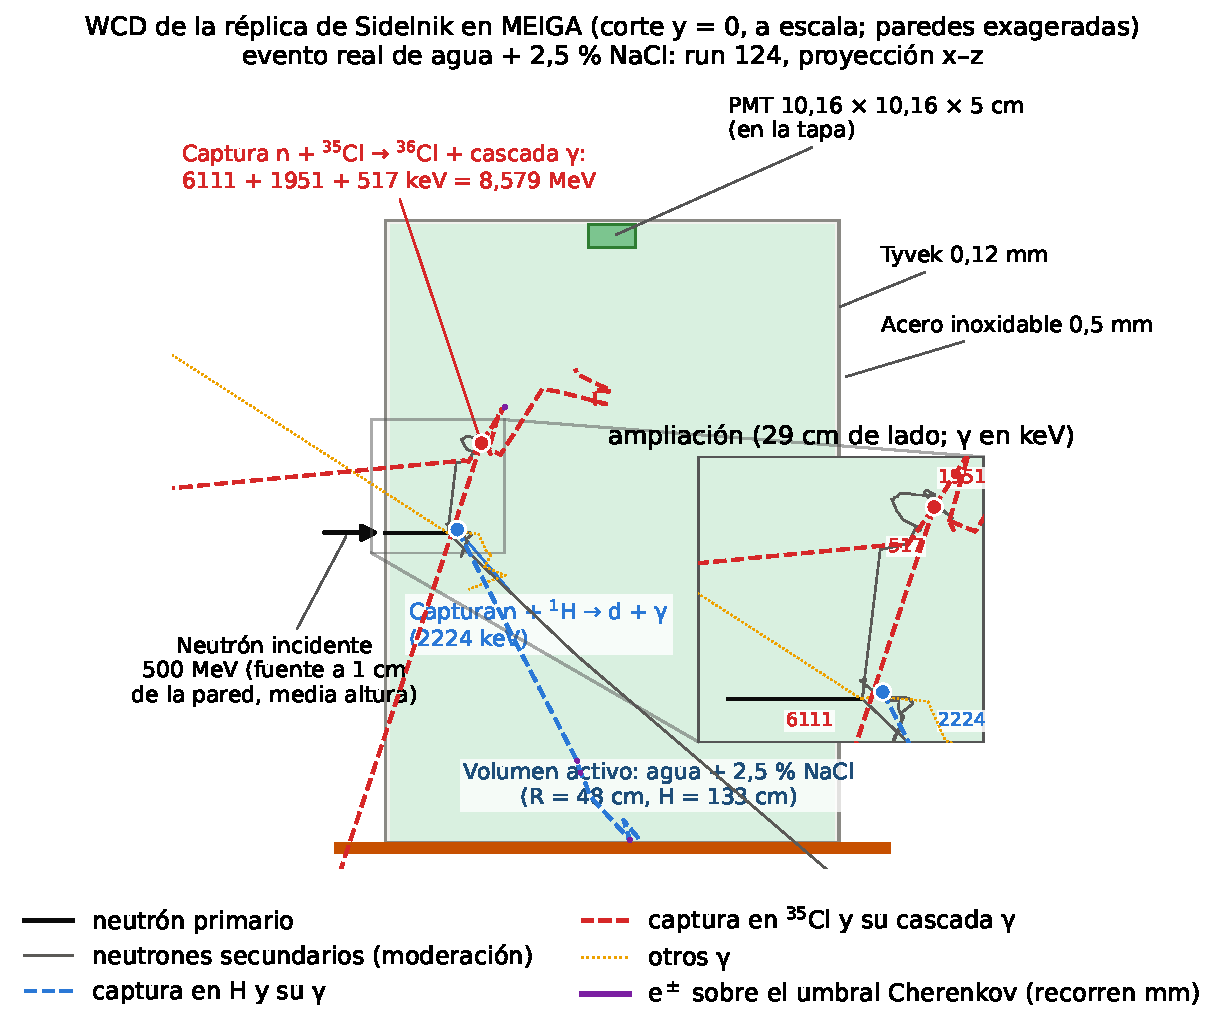
\includegraphics[width=\linewidth]{fig00_esquema_detector.pdf}
			\vspace{0.2cm}
			\captionsetup{width=\textwidth,justification=justified,singlelinecheck=false}
			\caption[Esquema del WCD simulado con un evento de neutrón de 500~MeV]{Esquema del WCD simulado (corte $y=0$, a escala; el espesor de las paredes está exagerado) con un evento real de la corrida de \textcolor{green}{agua + 2.5\,\% de NaCl}. El neutrón de 500~MeV entra a media altura y tiene una interacción inelástica; los neutrones secundarios se moderan y dos de ellos se capturan, uno en $^{1}$H (gamma de 2224~keV) y otro en $^{35}$Cl, con la cascada de 6111 + 1951 + 517~keV que conserva la energía de separación del neutrón (8.579~MeV). Los electrones de los gammas recorren pocos milímetros y emiten la luz Cherenkov. Equivalente a la Fig.~1 de \protect\citet{Sidelnik2020}, con la geometría y las trayectorias del presente modelo.}
			\label{fig:esquema-evento}
		\end{minipage}
	\end{adjustwidth}
\end{figure}

La comparación se organiza en tres niveles de exigencia: (i) magnitudes que deben coincidir en valor absoluto porque dependen solo de la física nuclear y de la geometría (energías de las líneas gamma, tiempos de captura, escala del espectro de electrones); (ii) magnitudes que se comparan mediante cocientes o formas normalizadas, porque los ejes del trabajo de referencia están en unidades arbitrarias o su normalización no se especifica (alturas relativas de líneas, espectros acumulados, histogramas de fotones); y (iii) tendencias con la concentración de NaCl, que no dependen de la normalización y constituyen la prueba más directa del objetivo de este trabajo.

%==========================================================
\section{Interacciones del neutrón primario de 500~MeV}
\label{subsubsec:primario}
%==========================================================

Antes de analizar la captura conviene seguir al neutrón incidente. A 500~MeV el neutrón primario solo experimenta tres procesos en el detector: dispersión elástica (\texttt{hadElastic}), interacción inelástica (\texttt{neutronInelastic}) y, raramente, captura. El núcleo blanco de cada interacción inelástica se reconstruyó por conservación de la carga y del número bariónico de los productos; los isótopos $^{17}$O (0.04\,\%) y $^{18}$O (0.21\,\%) aparecen con su abundancia natural, lo que valida la reconstrucción. La Tabla~(\ref{tab:destino-primario}) resume el destino del neutrón primario en los cuatro medios.

\begin{table}[!htbp]
	\centering
	\small
	\captionsetup{width=\linewidth,justification=justified,singlelinecheck=false}
	\caption[Destino del neutrón primario de 500~MeV]{Destino del neutrón primario de 500~MeV y localización de su interacción inelástica ($1.5\times10^{5}$ neutrones por medio).}
	\label{tab:destino-primario}
	\renewcommand{\arraystretch}{1.15}
	\resizebox{\textwidth}{!}{\begin{tabular}{lcccc}
		\toprule
		\textbf{Destino del neutrón primario} & \textcolor{red}{\textbf{Agua pura}} & \textcolor{green}{\textbf{2.5\,\% NaCl}} & \textcolor{violet}{\textbf{5\,\% NaCl}} & \textcolor{orange}{\textbf{10\,\% NaCl}} \\
		\midrule
		Atraviesa el tanque sin interactuar & 21.8\,\% & 21.3\,\% & 21.0\,\% & 20.0\,\% \\
		Interacción inelástica (la traza termina) & 61.7\,\% & 62.6\,\% & 62.9\,\% & 64.1\,\% \\
		Solo dispersiones elásticas y sale & 15.6\,\% & 15.3\,\% & 15.3\,\% & 15.1\,\% \\
		Solo dispersiones elásticas y es capturado & 0.88\,\% & 0.81\,\% & 0.78\,\% & 0.76\,\% \\
		\midrule
		Inelástica en el medio & 99.0\,\% & 99.0\,\% & 99.1\,\% & 99.1\,\% \\
		Inelástica en el acero / aire & 0.76 / 0.21\,\% & 0.75 / 0.20\,\% & 0.70 / 0.20\,\% & 0.69 / 0.17\,\% \\
		Blanco en el medio: $^{16}$O & 97.5\,\% & 95.2\,\% & 92.9\,\% & 88.3\,\% \\
		Blanco en el medio: $^{1}$H & 2.2\,\% & 2.1\,\% & 2.2\,\% & 2.0\,\% \\
		Blanco en el medio: $^{35}$Cl + $^{37}$Cl + $^{23}$Na & -- & 2.33\,\% & 4.64\,\% & 9.40\,\% \\
		Profundidad media de la inelástica (cm) & 40.2 & 40.2 & 40.0 & 39.8 \\
		\bottomrule
	\end{tabular}}
\end{table}

En la interacción inelástica, el modelo de cascada intranuclear de Bertini (\texttt{QGSP\_BERT\_HP}, por encima de $\approx$\,20~MeV) termina la traza del primario y crea trazas nuevas para todos los productos. La interacción ocurre casi siempre a la energía inicial: el 80\,\% de los primarios no sufre ninguna dispersión elástica previa. El 99\,\% de las inelásticas ocurre en el agua, distribuidas en todo el tanque y decreciendo con la profundidad (camino libre medio inelástico $\approx$\,1~m; Figura~\ref{fig:inelasticas-primario}a); el blanco es $^{16}$O en el 97\,\% de los casos y $^{1}$H en el 2.2\,\%, ya que la colisión neutrón--protón inelástica requiere producir un pion. Con NaCl, los núcleos de Cl y Na son el blanco en solo el 2.3\,\% (\textcolor{green}{2.5\,\%}), 4.6\,\% (\textcolor{violet}{5\,\%}) y 9.4\,\% (\textcolor{orange}{10\,\%}) de las inelásticas: la sal no modifica la fase de alta energía.

Cada inelástica produce en promedio 2.12 neutrones, 1.35 protones, 0.33 partículas $\alpha$, 0.12 deuterones, 2.0 gammas de desexcitación y 0.18 piones, y deja un núcleo residual en el 89\,\% de los casos ($^{12}$C, $^{15}$N, $^{15}$O, $^{14}$N, $^{8}$Be; Figura~\ref{fig:inelasticas-primario}d). La energía se reparte principalmente entre neutrones (280~MeV por inelástica) y protones (125~MeV). El neutrón más energético conserva en mediana el 48\,\% de la energía incidente y puede producir a su vez otra inelástica, de modo que cada evento contiene en promedio 3.44 neutrones en agua pura. Los neutrones que terminan capturados son los de evaporación, de pocos MeV, que se moderan en el agua. Los núcleos residuales emisores $\beta^{+}$ ($^{15}$O, $^{13}$N y $^{11}$C) son además la fuente de la línea de aniquilación de larga vida discutida en la Sec.~\ref{subsubsec:espectros-gamma}, y los gammas de desexcitación de $^{12}$C, $^{15}$N y $^{16}$O forman el fondo de 4--7~MeV discutido en la Sec.~\ref{subsubsec:electrones}. Las multiplicidades y los núcleos residuales coinciden en los cuatro medios dentro del 2\,\%.

\begin{figure}[!htbp]
	\begin{adjustwidth}{0cm}{0cm}
		\centering
		\begin{minipage}{\linewidth}
			\centering
			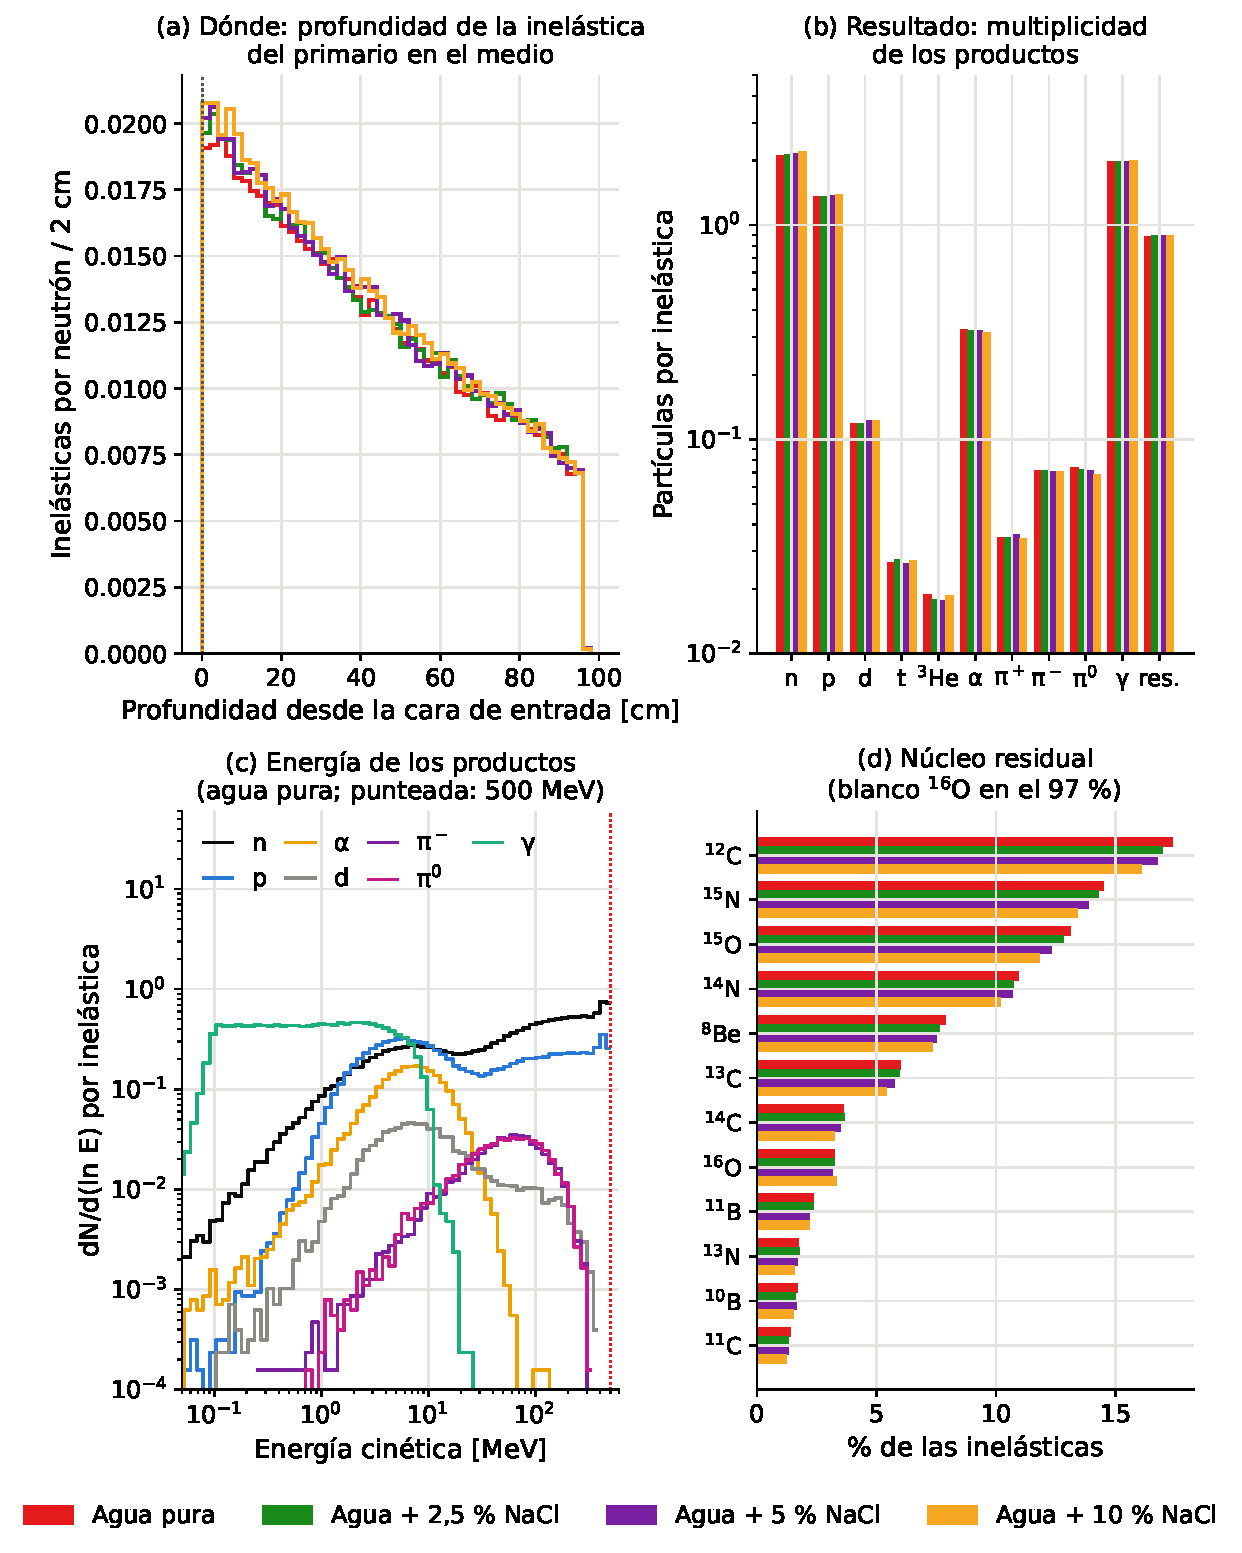
\includegraphics[width=\linewidth]{fig20_inelasticas_primario.pdf}
			\vspace{0.2cm}
			\captionsetup{width=\textwidth,justification=justified,singlelinecheck=false}
			\caption[Interacciones inelásticas del neutrón primario de 500~MeV]{Interacciones inelásticas del neutrón primario de 500~MeV: (a) profundidad a lo largo del haz; (b) multiplicidad media de los productos; (c) espectro de energía de los productos en \textcolor{red}{agua pura}; (d) núcleos residuales más frecuentes.}
			\label{fig:inelasticas-primario}
		\end{minipage}
	\end{adjustwidth}
\end{figure}

\paragraph{El neutrón capturado no es el primario:} Solo el 0.88\,\% (\textcolor{red}{agua pura}), 0.81\,\% (\textcolor{green}{2.5\,\%}), 0.78\,\% (\textcolor{violet}{5\,\%}) y 0.76\,\% (\textcolor{orange}{10\,\%}) de los primarios se captura como la misma traza, después de frenarse únicamente por dispersiones elásticas. En cambio, en el 97\,\% de los eventos con captura el primario tuvo antes una interacción inelástica: los neutrones capturados son los secundarios. Este comportamiento no es propio del presente modelo, sino de cualquier simulación con \textsc{Geant4}, incluida la del trabajo de referencia, porque los modelos de cascada intranuclear terminan la traza incidente; además, los neutrones son partículas indistinguibles y, después de la inelástica, carece de sentido preguntar si se capturó ``el primario''. En consecuencia, la probabilidad de captura debe definirse sobre el conjunto de neutrones del evento, como se discute en la Sec.~\ref{subsubsec:captura}.

\paragraph{Inventario de procesos:} El Apéndice~\ref{ap:procesos-neutrones} reúne, para cada medio, todas las reacciones de los neutrones en el volumen del detector, primarios y secundarios (Tablas~\ref{tab:procesos_pura}--\ref{tab:procesos_nacl10}): la ecuación de la reacción, su valor $Q$, la energía típica del neutrón, su porcentaje dentro de cada tipo de proceso y los gammas que emite. Estas tablas constituyen el inventario a partir del cual se interpretan las secciones siguientes. En \textcolor{red}{agua pura}, la dispersión elástica en $^{1}$H representa el 84\,\% de las colisiones con blanco identificado y es la responsable de la moderación; la captura ocurre en $^{1}$H en el 99.9\,\% de los casos; y entre las interacciones inelásticas dominan la dispersión inelástica $^{16}$O(n,n$'$) y los canales $^{16}$O(n,n$\alpha$)$^{12}$C, $^{16}$O(n,np)$^{15}$N y $^{16}$O(n,2n)$^{15}$O, que emiten las líneas de desexcitación de 4.44, 6.13, 6.92 y 7.12~MeV y producen los emisores $\beta^{+}$ de larga vida. Con NaCl se añaden la captura en $^{35}$Cl, con su cascada de 517 a 8579~keV, y, en mucha menor proporción, las reacciones en $^{23}$Na y $^{37}$Cl. Las diferencias con el trabajo de referencia en el fondo de gammas de 4--7~MeV y en la línea de 0.511~MeV (Secs.~\ref{subsubsec:espectros-gamma} y \ref{subsubsec:electrones}) tienen su origen en estos canales inelásticos.

%==========================================================
\section{Moderación de los neutrones: dispersiones elásticas}
\label{subsubsec:elasticas}
%==========================================================

Las dispersiones elásticas son el mecanismo que modera a los neutrones antes de la captura. Se reconstruyeron todos los vértices elásticos de todos los neutrones: 15\,573\,769 en \textcolor{red}{agua pura} (104 por neutrón incidente), 12\,519\,457 en \textcolor{green}{agua + 2.5\,\% de NaCl} (83 por neutrón), 10\,732\,779 en \textcolor{violet}{agua + 5\,\% de NaCl} (72 por neutrón) y 8\,834\,631 en \textcolor{orange}{agua + 10\,\% de NaCl} (59 por neutrón). Con sal hay menos vértices porque el cloro captura antes a los neutrones térmicos: la fracción de vértices por debajo de 1~eV es del 74\,\%, 69\,\%, 65\,\% y 59\,\%, respectivamente. Cada vértice corresponde a la reacción
\begin{equation}
	n(E_{\mathrm{in}},\hat{d}_{\mathrm{in}}) + (A,Z) \longrightarrow n(E_{\mathrm{out}},\hat{d}_{\mathrm{out}}) + (A,Z)_{\mathrm{retroceso}} .
\end{equation}

\noindent La Figura~(\ref{fig:elasticas}) resume la reconstrucción de estos vértices. Cada panel responde a una pregunta sobre la moderación: con qué núcleo choca el neutrón (paneles a y b), cuánta energía pierde y en qué dirección sale (paneles c, d y e) y si la simulación respeta las leyes de conservación (panel f).

\begin{figure}[!htbp]
	\begin{adjustwidth}{0cm}{0cm}
		\centering
		\begin{minipage}{\linewidth}
			\centering
			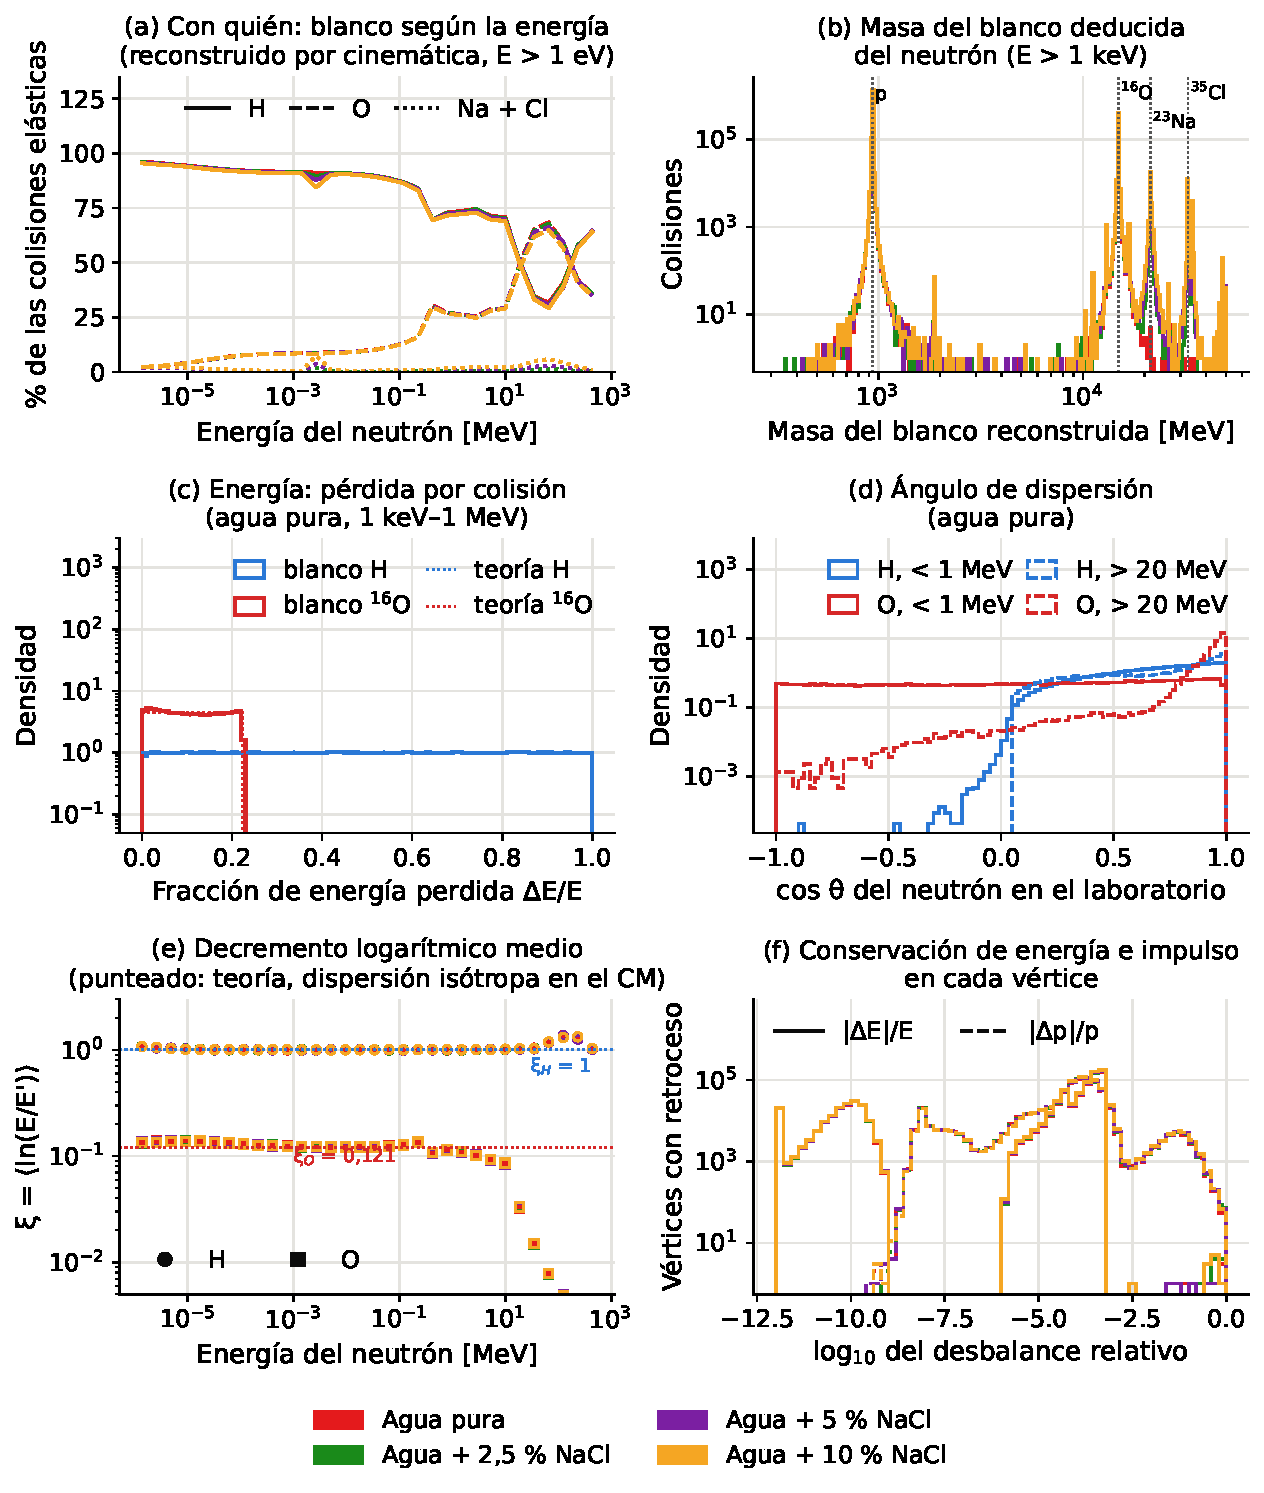
\includegraphics[width=\linewidth]{fig21_elasticas.pdf}
			\vspace{0.2cm}
			\captionsetup{width=\textwidth,justification=justified,singlelinecheck=false}
			\caption[Reconstrucción de los vértices de dispersión elástica]{Reconstrucción de los vértices de dispersión elástica: (a) núcleo blanco según la energía del neutrón; (b) masa del blanco deducida solo de la cinemática del neutrón; (c) fracción de energía perdida por colisión en H y $^{16}$O frente a la teoría; (d) ángulo de dispersión en el laboratorio; (e) decremento logarítmico medio $\xi$; (f) balance de energía e impulso en cada vértice.}
			\label{fig:elasticas}
		\end{minipage}
	\end{adjustwidth}
\end{figure}

\paragraph{Con quién: el núcleo blanco.} A partir de la transferencia de impulso $\vec{q}=\vec{p}_{\mathrm{in}}-\vec{p}_{\mathrm{out}}$ y de energía $T=E_{\mathrm{in}}-E_{\mathrm{out}}$ del neutrón, la masa del núcleo blanco se obtiene sin usar el núcleo de retroceso como
\begin{equation}
	M = \frac{q^{2}-T^{2}}{2T}.
\end{equation}
\noindent La distribución de $M$ (Figura~\ref{fig:elasticas}b) presenta picos estrechos en la masa del protón (938.27~MeV) y del núcleo de $^{16}$O (14\,895.1~MeV) y, en los medios con NaCl, en las de $^{23}$Na y $^{35}$Cl. En el 100\,\% de los vértices con retroceso registrado, el blanco reconstruido coincide con la partícula de retroceso. Por debajo de 20~MeV las masas reconstruidas son las \emph{atómicas} (938.78 y 14\,899.1~MeV), porque el modelo de alta precisión \texttt{G4NeutronHP} trabaja con masas atómicas, mientras que por encima de 20~MeV los modelos hadrónicos usan masas nucleares. La composición por energía (Figura~\ref{fig:elasticas}a y Tabla~\ref{tab:elasticas}) sigue las secciones eficaces elásticas: el hidrógeno es el blanco en el 86--88\,\% de las colisiones por debajo de 1~MeV, mientras que por encima de 20~MeV el oxígeno pasa a ser el blanco más frecuente (44.8\,\%), porque la sección eficaz n--p decrece rápidamente con la energía.

\begin{table}[!htbp]
	\centering
	\small
	\captionsetup{width=\linewidth,justification=justified,singlelinecheck=false}
	\caption[Vértices de dispersión elástica y decremento logarítmico medio]{Vértices de dispersión elástica por intervalo de energía en \textcolor{red}{agua pura}, núcleo blanco reconstruido por cinemática y decremento logarítmico medio $\xi$. Por debajo de 1~eV (11\,466\,643 vértices) el blanco térmico no está en reposo y no se reconstruye.}
	\label{tab:elasticas}
	\renewcommand{\arraystretch}{1.15}
	\begin{tabular}{lcccc}
		\toprule
		\textbf{Energía del neutrón} & \textbf{Vértices} & \textbf{Blanco H / O} & $\boldsymbol{\xi_{\mathrm{H}}}$ & $\boldsymbol{\xi_{\mathrm{O}}}$ \\
		\midrule
		1 eV -- 1 keV & 1\,002\,307 & 88.2\,\% / 5.5\,\% & 1.017 & 0.131 \\
		1 keV -- 1 MeV & 1\,083\,824 & 85.6\,\% / 14.2\,\% & 1.000 & 0.118 \\
		1 -- 20 MeV & 413\,486 & 70.7\,\% / 28.4\,\% & 1.007 & 0.094 \\
		$>$ 20 MeV & 194\,087 & 33.6\,\% / 44.8\,\% & 1.106 & 0.011 \\
		\midrule
		Teoría (dispersión isótropa en el CM) & & & 1.000 & 0.121 \\
		\bottomrule
	\end{tabular}
\end{table}

\paragraph{Energía y ángulo.} En una colisión elástica con un núcleo en reposo y dispersión isótropa en el sistema del centro de masas (CM), la energía final del neutrón se distribuye uniformemente entre $\alpha E$ y $E$, con
\begin{equation}
	\alpha=\left(\frac{A-1}{A+1}\right)^{2},
\end{equation}
de modo que la fracción de energía perdida $\Delta E/E$ es uniforme entre 0 y $1-\alpha$. La Figura~(\ref{fig:elasticas}c) muestra exactamente este comportamiento entre 1~keV y 1~MeV: para el H ($\alpha=0$) la pérdida es uniforme entre 0 y 1, es decir, en una sola colisión el neutrón puede perder toda su energía, y para el $^{16}$O ($\alpha=0.777$) es uniforme entre 0 y $1-\alpha=0.223$. La misma cinemática fija el ángulo de dispersión en el laboratorio (Figura~\ref{fig:elasticas}d). La Figura~(\ref{fig:esquema-cinematica}) explica gráficamente estos resultados: en la colisión con $^{1}$H, de masa casi igual a la del neutrón, el neutrón y el protón salen en direcciones perpendiculares ($\theta+\phi=90^{\circ}$), por lo que el neutrón nunca retrocede (panel a); en la colisión con $^{16}$O el neutrón puede rebotar hacia atrás, pero conserva al menos el 78\,\% de su energía (panel b). El diagrama de velocidades (panel c) muestra el origen de esta diferencia: la velocidad final en el laboratorio es la suma de la velocidad del centro de masas, $V_{CM}=v/(A+1)$, y de la velocidad del neutrón en el CM, $u'=Av/(A+1)$, que, al ser la dispersión isótropa en el CM, puede apuntar en cualquier dirección sobre un círculo de radio $u'$. Para el H ($A=1$) el círculo pasa por el origen y la velocidad final nunca apunta hacia atrás; para el $^{16}$O ($A\approx16$) el origen queda dentro del círculo y cualquier dirección es posible. Para el H, el neutrón no puede retroceder: $\cos\theta_{\mathrm{lab}}$ está entre 0 y 1, con densidad $2\cos\theta_{\mathrm{lab}}$ y valor medio $\langle\cos\theta_{\mathrm{lab}}\rangle=2/(3A)=0.67$. Para el $^{16}$O la distribución es casi plana entre $-1$ y 1, con $\langle\cos\theta_{\mathrm{lab}}\rangle=0.04$. Por encima de 20~MeV el comportamiento cambia para el oxígeno: su distribución se concentra hacia $\cos\theta_{\mathrm{lab}}\approx1$, porque la dispersión deja de ser isótropa en el CM y se vuelve frontal (difracción), de modo que el neutrón rápido apenas cambia de dirección ni de energía al chocar con el O. En el H, en cambio, la distribución sigue cercana a la de la dispersión isótropa en el CM (Figura~\ref{fig:esquema-cinematica}f).

\begin{figure}[!htbp]
	\centering
	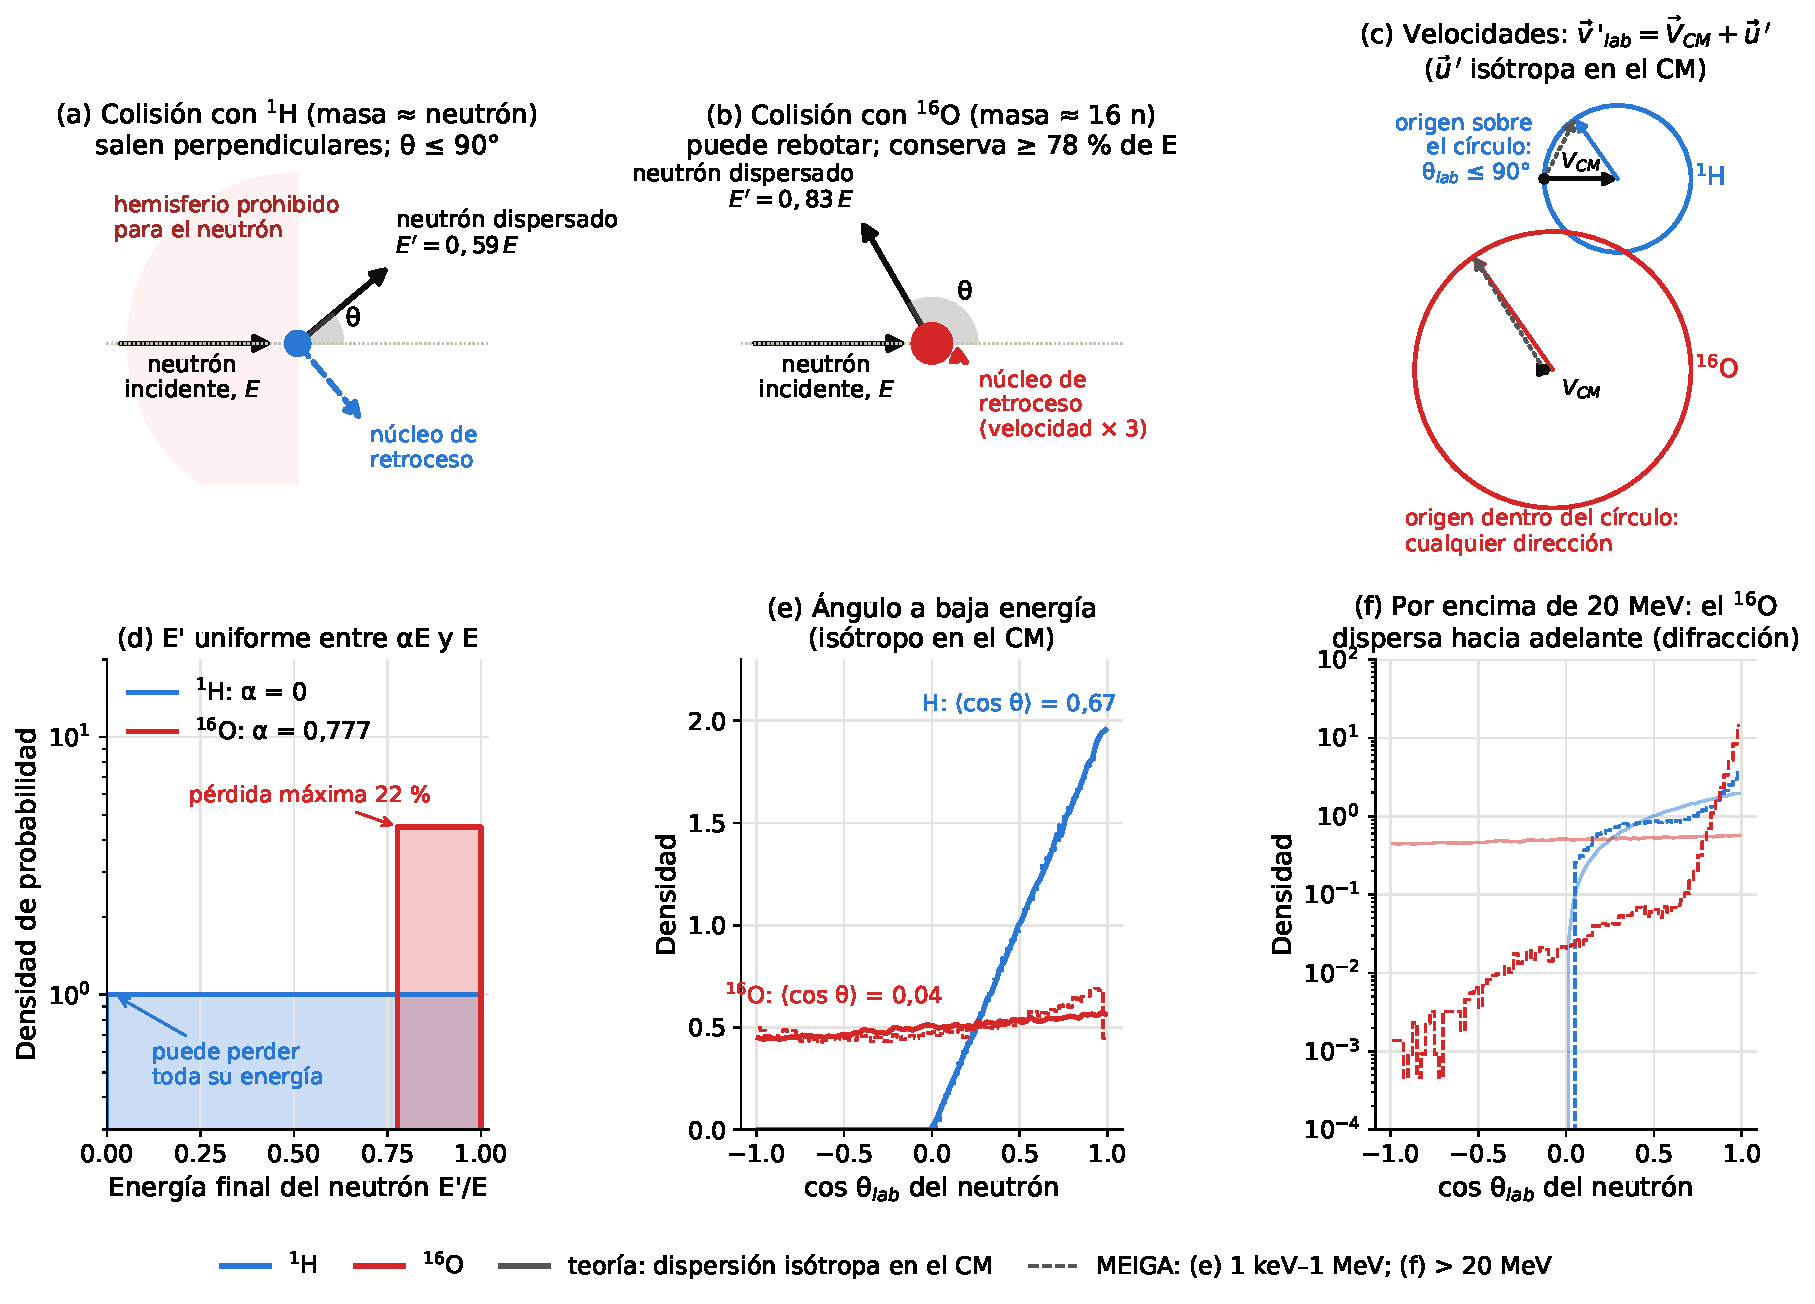
\includegraphics[width=\linewidth]{fig23_esquema_cinematica_elastica.pdf}
	\vspace{0.2cm}
	\captionsetup{width=\textwidth,justification=justified,singlelinecheck=false}
	\caption[Cinemática de la dispersión elástica de neutrones en H y $^{16}$O]{Cinemática de la dispersión elástica de neutrones en el laboratorio. (a) Colisión con $^{1}$H: el neutrón y el protón salen perpendiculares y el neutrón no puede retroceder (región sombreada). (b) Colisión con $^{16}$O: el neutrón puede rebotar y conserva al menos el 78\,\% de su energía; la velocidad del núcleo de retroceso se muestra multiplicada por 3. (c) Diagrama de velocidades: $\vec v\,'_{\mathrm{lab}}=\vec V_{CM}+\vec u\,'$, con $\vec u\,'$ isótropa sobre el círculo de radio $u'$. (d) Distribución de la energía final, uniforme entre $\alpha E$ y $E$. (e) Distribución de $\cos\theta_{\mathrm{lab}}$ entre 1~keV y 1~MeV: teoría (dispersión isótropa en el CM) frente a la simulación en \textcolor{red}{agua pura}. (f) Por encima de 20~MeV: el $^{16}$O dispersa hacia adelante (difracción), mientras que el H permanece cercano a la dispersión isótropa en el CM.}
	\label{fig:esquema-cinematica}
\end{figure}

El decremento logarítmico medio resume la pérdida de energía por colisión:
\begin{equation}
	\xi = \left\langle \ln\frac{E}{E'}\right\rangle = 1 + \frac{\alpha\ln\alpha}{1-\alpha}.
\end{equation}
\noindent Entre 1~keV y 1~MeV se obtiene $\xi_{\mathrm{H}}=1.000$ (teoría: 1) y $\xi_{\mathrm{O}}=0.118$ (teoría: 0.121), y ambos valores se mantienen constantes desde el eV hasta unos MeV (Figura~\ref{fig:elasticas}e y Tabla~\ref{tab:elasticas}). Con ellos, el número medio de colisiones necesarias para moderar un neutrón de evaporación de 2~MeV hasta la energía térmica (0.025~eV) es $n=\ln(E_{0}/E_{\mathrm{th}})/\xi\approx18$ en H y $\approx150$ en $^{16}$O. Por encima de 20~MeV $\xi_{\mathrm{O}}$ cae a 0.011, por la dispersión frontal, mientras que $\xi_{\mathrm{H}}$ sube (1.1). En consecuencia, los neutrones rápidos se moderan casi exclusivamente en el hidrógeno. Con NaCl, el Na y el Cl son el blanco en solo el 0.6\,\% (\textcolor{green}{2.5\,\%}), 1.0\,\% (\textcolor{violet}{5\,\%}) y 1.7\,\% (\textcolor{orange}{10\,\%}) de las colisiones, y la cinemática (masas reconstruidas, $\xi$ y conservación) coincide en los cuatro medios dentro de 0.002: \emph{la sal modifica la captura, no la moderación}.

\paragraph{Neutrones térmicos.} El 74\,\% de los vértices en \textcolor{red}{agua pura} (11\,466\,643) ocurre por debajo de 1~eV, cuando el neutrón ya está termalizado y difunde por el agua hasta ser capturado. En este régimen el núcleo blanco no está en reposo: su energía térmica ($\sim kT=0.025$~eV) es comparable a la del neutrón, y la simulación la describe con el modelo de gas libre, porque estas corridas no incluyen la dispersión térmica $S(\alpha,\beta)$ que tiene en cuenta los enlaces moleculares del agua. Por ello el 44\,\% de las colisiones \emph{aumenta} la energía del neutrón, que intercambia energía con el medio hasta alcanzar el equilibrio térmico (mediana de la energía al capturarse: 30.5~meV, Tabla~\ref{tab:efecto-nacl-captura}). La reconstrucción con el blanco en reposo no es válida en este régimen y no se aplica; además, \textsc{Geant4} no registra el núcleo de retroceso por debajo de $\approx$\,1~keV. Las pequeñas desviaciones de $\xi$ entre 1~eV y 1~keV (1.017 para el H y 0.131 para el O) son el comienzo de este efecto térmico.

\paragraph{Leyes de conservación.} En cada vértice con retroceso registrado se verificó el balance de energía y de impulso entre el estado inicial (neutrón incidente y núcleo en reposo) y el final (neutrón dispersado y núcleo de retroceso) (Figura~\ref{fig:elasticas}f). La energía se conserva dentro de una parte en $10^{3}$ en el 99.998\,\% de los vértices; el residuo típico, de $\sim5\times10^{-4}$, proviene de la convención de masas atómicas del modelo de alta precisión. El impulso se conserva dentro del 1\,\% en el 96.7\,\% de los vértices (mediana del desbalance relativo $1.2\times10^{-4}$); el resto corresponde a núcleos de retroceso cuyo primer paso es tan corto que su dirección queda mal definida, no a una violación física. La carga, el número bariónico y el número leptónico se conservan exactamente, porque el estado inicial y el final contienen el mismo neutrón y el mismo núcleo, y no aparecen núcleos de retroceso distintos de los del medio ($p$, $^{16,17,18}$O, $^{23}$Na, $^{35,37}$Cl), salvo en el Tyvek ($^{12}$C), el acero ($^{56}$Fe, $^{52}$Cr), el aire ($^{14}$N) y algunos deuterones del $^{2}$H natural del agua. Estos controles confirman que la moderación simulada respeta la cinemática de la dispersión elástica de dos cuerpos.

%==========================================================
\section{Probabilidad, tiempo y distancia de captura}
\label{subsubsec:captura}
%==========================================================

\citet[Sec.~3, Tabla~2, p.~2218]{Sidelnik2020} reportan la fracción de capturas de neutrones dentro del volumen activo sin especificar sobre qué total se calcula. La Tabla~(\ref{tab:defs-captura}) compara tres definiciones posibles. La captura de la traza primaria (0.88\,\%) mide la numeración de las trazas en \textsc{Geant4} y no es comparable con el trabajo de referencia. La magnitud comparable es el número de capturas en el agua dividido por todos los neutrones del evento (primario y secundarios): 24.08\,\% en \textcolor{red}{agua pura}, frente al 25.18\,\% de Sidelnik et al. En otras palabras, de cada cuatro neutrones presentes en el tanque, uno termina capturado en el agua; los demás escapan o desaparecen en interacciones inelásticas. Para la eficiencia del detector, la magnitud relevante es, en cambio, la fracción de neutrones incidentes que producen al menos una captura: 42.4\,\% en \textcolor{red}{agua pura}.

\begin{table}[!htbp]
	\centering
	\small
	\captionsetup{width=\linewidth,justification=justified,singlelinecheck=false}
	\caption[Definiciones de la probabilidad de captura de neutrones]{Tres definiciones de la probabilidad de captura de neutrones en el volumen activo. Solo la tercera es comparable con la Tabla~2 de \protect\citet{Sidelnik2020}; entre paréntesis, el cambio relativo respecto al \textcolor{red}{agua pura}.}
	\label{tab:defs-captura}
	\renewcommand{\arraystretch}{1.15}
	\resizebox{\textwidth}{!}{
	\begin{tabular}{lcccc}
		\toprule
		 & \textcolor{red}{\textbf{Agua pura}} & \textcolor{green}{\textbf{2.5\,\% NaCl}} & \textcolor{violet}{\textbf{5\,\% NaCl}} & \textcolor{orange}{\textbf{10\,\% NaCl}} \\
		\midrule
		Primario capturado (misma traza) & 0.88\,\% & 0.81\,\% & 0.78\,\% & 0.76\,\% \\
		Neutrones incidentes con $\geq 1$ captura en el agua & 42.4\,\% & 43.3\,\% (+2.0\,\%) & 44.3\,\% (+4.3\,\%) & 45.9\,\% (+8.3\,\%) \\
		\textbf{Capturas / neutrones del evento (este trabajo)} & \textbf{24.08\,\%} & \textbf{24.59\,\%} (+2.1\,\%) & \textbf{25.19\,\%} (+4.6\,\%) & \textbf{26.08\,\%} (+8.3\,\%) \\
		\textit{Sidelnik et al.: probabilidad de captura} & \textit{25.18\,\%} & \textit{26.73\,\%} (+6.2\,\%) & \textit{27.65\,\%} (+9.8\,\%) & \textit{29.26\,\%} (+16.2\,\%) \\
		\midrule
		Capturas en el agua por neutrón incidente & 0.829 & 0.864 (+4.3\,\%) & 0.903 (+8.9\,\%) & 0.972 (+17.3\,\%) \\
		Neutrones por evento (primario + secundarios) & 3.44 & 3.51 & 3.58 & 3.73 \\
		\bottomrule
	\end{tabular}}
\end{table}

En \textcolor{red}{agua pura} la probabilidad de captura queda 1.1 puntos por debajo del trabajo de referencia (5\,\% relativo), una diferencia razonable entre dos simulaciones con versiones y modelos hadrónicos distintos. Con NaCl la tendencia es la misma que en el trabajo de referencia, monótona con la concentración, pero aproximadamente dos veces más débil: +2.1\,\%, +4.6\,\% y +8.3\,\% frente a +6.2\,\%, +9.8\,\% y +16.2\,\%. Esta diferencia no puede atribuirse a la estadística (con 2.5\,\% de NaCl el aumento es significativo a $\approx$\,6$\sigma$) ni a un error de configuración, porque el tiempo de captura sigue exactamente la predicción de las secciones eficaces térmicas (Tabla~\ref{tab:efecto-nacl-captura}). Puede deberse a diferencias en las secciones eficaces del cloro o en la normalización de Sidelnik et al., que el artículo no detalla.

\paragraph{Efecto del NaCl en la captura:} La Tabla~(\ref{tab:efecto-nacl-captura}) resume el efecto de la sal. El tiempo característico de captura, obtenido del ajuste exponencial de la distribución de tiempos (Figura~\ref{fig:tiempo-captura}), puede estimarse a partir de las secciones eficaces térmicas de captura de los núcleos del medio como
\begin{equation}
	\tau = \frac{1}{v_{0}\sum_{i} N_{i}\,\sigma_{0,i}},
	\label{eq:tau-captura}
\end{equation}
donde $v_{0}=2200$~m/s es la velocidad de referencia de los neutrones térmicos, $N_{i}$ la densidad de núcleos del isótopo $i$ y $\sigma_{0,i}$ su sección eficaz térmica de captura (Tabla~\ref{elem-capt-neut}). La simulación reproduce la reducción de $\tau$ con la concentración dentro del 6\,\% en los cuatro medios (de 192 a 75~µs, frente a 205 y 78~µs). La fracción de capturas en $^{35}$Cl es, en cambio, mayor que la predicha por las mismas secciones eficaces (35.8, 51.5 y 67.7\,\% frente a 28.0, 44.2 y 62.2\,\%), un exceso relativo que disminuye con la concentración y ya observado en las campañas anteriores con G4NDL~4.6.

\begin{table}[!htbp]
	\centering
	\small
	\captionsetup{width=\linewidth,justification=justified,singlelinecheck=false}
	\caption[Efecto del NaCl en la captura de neutrones]{Captura de neutrones en los distintos medios ($1.5\times10^{5}$ neutrones de 500~MeV por medio) frente a las predicciones de las secciones eficaces térmicas y a las tendencias de \protect\citet{Sidelnik2020}. Entre paréntesis, el cambio relativo respecto al \textcolor{red}{agua pura}.}
	\label{tab:efecto-nacl-captura}
	\renewcommand{\arraystretch}{1.15}
	\resizebox{\textwidth}{!}{
	\begin{tabular}{lcccc}
		\toprule
		 & \textcolor{red}{\textbf{Agua pura}} & \textcolor{green}{\textbf{2.5\,\% NaCl}} & \textcolor{violet}{\textbf{5\,\% NaCl}} & \textcolor{orange}{\textbf{10\,\% NaCl}} \\
		\midrule
		Capturas en $^{1}$H & 99.94\,\% & 63.5\,\% & 47.5\,\% & 31.0\,\% \\
		Capturas en $^{35}$Cl (este trabajo) & -- & 35.8\,\% & 51.5\,\% & 67.7\,\% \\
		\quad teoría (secciones eficaces térmicas) & -- & 28.0\,\% & 44.2\,\% & 62.2\,\% \\
		Capturas en $^{23}$Na / $^{37}$Cl & -- & 0.6 / 0.1\,\% & 0.8 / 0.2\,\% & 1.1 / 0.2\,\% \\
		Tiempo de captura $\tau$ (µs), este trabajo & 192 & 140 ($-$27.0\,\%) & 109 ($-$43.2\,\%) & 75 ($-$61.0\,\%) \\
		\quad teoría, Ec.~(\ref{eq:tau-captura}) (µs) & 205 & 147 ($-$28.0\,\%) & 114 ($-$44.2\,\%) & 78 ($-$62.1\,\%) \\
		Energía del neutrón al capturarse, mediana (meV) & 30.5 & 30.6 & 31.0 & 31.7 \\
		Energía gamma de captura por neutrón incidente (MeV) & 1.85 & 4.39 & 5.71 & 7.40 \\
		\bottomrule
	\end{tabular}}
\end{table}

\begin{figure}[!htbp]
	\begin{adjustwidth}{0cm}{0cm}
		\centering
		\begin{minipage}{\linewidth}
			\centering
			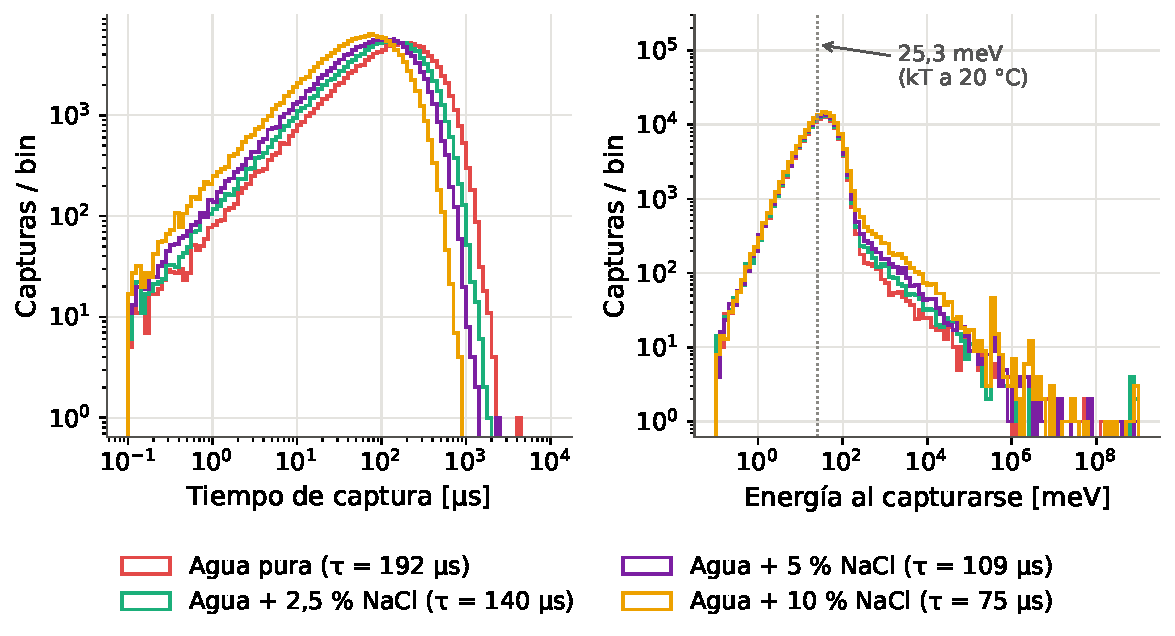
\includegraphics[width=\linewidth]{fig05_tiempo_energia_captura.pdf}
			\vspace{0.2cm}
			\captionsetup{width=\textwidth,justification=justified,singlelinecheck=false}
			\caption[Tiempo de captura y energía del neutrón al capturarse]{Distribución del tiempo de captura (izquierda) y de la energía del neutrón en el momento de la captura (derecha; la línea punteada marca la energía térmica de referencia, 25.3~meV, $kT$ a 20~°C) para \textcolor{red}{agua pura}, \textcolor{green}{agua + 2.5\,\% de NaCl}, \textcolor{violet}{agua + 5\,\% de NaCl} y \textcolor{orange}{agua + 10\,\% de NaCl}.}
			\label{fig:tiempo-captura}
		\end{minipage}
	\end{adjustwidth}
\end{figure}

\paragraph{Distancia de máxima absorción:} \citet[Sec.~3, Fig.~2]{Sidelnik2020} reportan la distribución de capturas en función de la distancia desde el borde del tanque, con un máximo a 8.4~cm en \textcolor{red}{agua pura}. Medida a lo largo del haz desde la cara de entrada, la distribución de capturas del presente modelo es, en cambio, una joroba ancha con máximo cerca del centro del tanque (46.5~cm), porque el primario realiza su primera inelástica a 40~cm de profundidad en promedio y los neutrones de la cascada se capturan en todo el volumen (Figura~\ref{fig:distancia-captura}). La forma de la Fig.~2 de Sidelnik et al., con un máximo cercano y una cola larga, aparece si la distancia se mide desde el punto donde nace el neutrón capturado (Tabla~\ref{tab:distancia-captura}). Esto sugiere que la distancia reportada en el trabajo de referencia describe la escala de moderación. Con esta definición, la distancia disminuye con la concentración de NaCl, como en el trabajo de referencia.

\begin{table}[!htbp]
	\centering
	\small
	\captionsetup{width=\linewidth,justification=justified,singlelinecheck=false}
	\caption[Distancia de máxima absorción de neutrones]{Distancia de máxima absorción con tres definiciones (máximo del histograma suavizado con bines de 0.5~cm), frente a la Fig.~2 de \protect\citet{Sidelnik2020}.}
	\label{tab:distancia-captura}
	\renewcommand{\arraystretch}{1.15}
	\resizebox{\textwidth}{!}{
	\begin{tabular}{lcccc}
		\toprule
		\textbf{Distancia de máxima absorción (cm)} & \textcolor{red}{\textbf{Agua pura}} & \textcolor{green}{\textbf{2.5\,\% NaCl}} & \textcolor{violet}{\textbf{5\,\% NaCl}} & \textcolor{orange}{\textbf{10\,\% NaCl}} \\
		\midrule
		Cara de entrada $\to$ captura, a lo largo del haz & 46.5 & 45.3 & 36.1 & 47.8 \\
		Vértice del neutrón capturado $\to$ captura & 11.1 & 10.0 ($-$10\,\%) & 9.8 ($-$12\,\%) & 9.6 ($-$14\,\%) \\
		Inelástica del primario $\to$ captura & 12.7 & 11.3 & 11.2 & 10.4 \\
		\textit{Sidelnik et al.} & \textit{8.4} & \textit{8.0} ($-$5\,\%) & \textit{7.7} ($-$8\,\%) & \textit{7.3} ($-$13\,\%) \\
		\bottomrule
	\end{tabular}}
\end{table}

\begin{figure}[!htbp]
	\begin{adjustwidth}{0cm}{0cm}
		\centering
		\begin{minipage}{\linewidth}
			\centering
			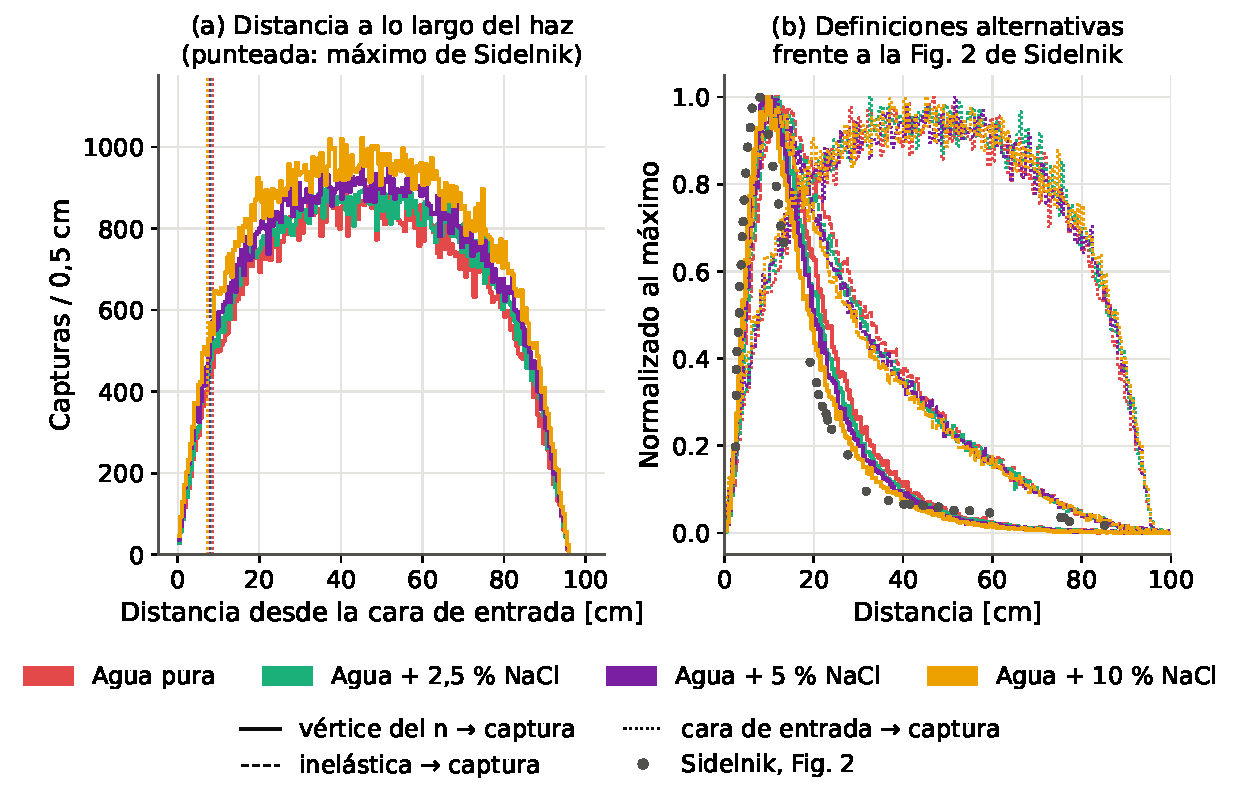
\includegraphics[width=\linewidth]{fig01_distancia_captura.pdf}
			\vspace{0.2cm}
			\captionsetup{width=\textwidth,justification=justified,singlelinecheck=false}
			\caption[Distancia de captura de los neutrones]{Izquierda: capturas en función de la distancia a lo largo del haz desde la cara de entrada. Derecha: distribuciones normalizadas con las tres definiciones de distancia de la Tabla~\ref{tab:distancia-captura}, frente a la curva de \textcolor{red}{agua pura} digitalizada de la Fig.~2 de \protect\citet{Sidelnik2020} (puntos).}
			\label{fig:distancia-captura}
		\end{minipage}
	\end{adjustwidth}
\end{figure}

%==========================================================
\section{Contribución de los principales núcleos a la captura de neutrones}
\label{subsubsec:nucleos-captura-neutrones}
%==========================================================

La identificación de los núcleos que participan en los procesos de captura constituye un aspecto fundamental para comprender la modificación de la respuesta del WCD cuando el agua es dopada con NaCl. La captura conduce a la formación de un núcleo compuesto excitado que posteriormente se desexcita mediante la emisión de uno o varios fotones gamma. En el caso del agua pura, la absorción de neutrones ocurre principalmente en los núcleos de $^{1}$H y, en menor medida, en $^{16}$O. Cuando se incorpora NaCl al volumen detector aparecen nuevos núcleos capaces de participar en el proceso de captura, entre los cuales se encuentran $^{35}$Cl, $^{37}$Cl y $^{23}$Na. Se consideran los medios de \textcolor{red}{agua pura} (\textcolor{red}{rojo}), \textcolor{green}{agua + 2.5\,\% de NaCl} (\textcolor{green}{verde}), \textcolor{violet}{agua + 5\,\% de NaCl} (\textcolor{violet}{violeta}) y \textcolor{orange}{agua + 10\,\% de NaCl} (\textcolor{orange}{naranja}).

La Figura~(\ref{fig-lineas-esp-1}) presenta los gammas emitidos en cada captura, enlazados con el núcleo que capturó el neutrón. A diferencia de la versión anterior de esta figura, la intensidad se expresa en fotones por 100 capturas y se compara directamente con los valores de referencia: \citet{Firestone2016} para $^{16}$O y la evaluación ENSDF \citep{Nica2012} para $^{35}$Cl.

\begin{figure}[!htbp]
	\begin{adjustwidth}{0cm}{0cm}
		\centering
		\begin{minipage}{\linewidth}
			\centering
			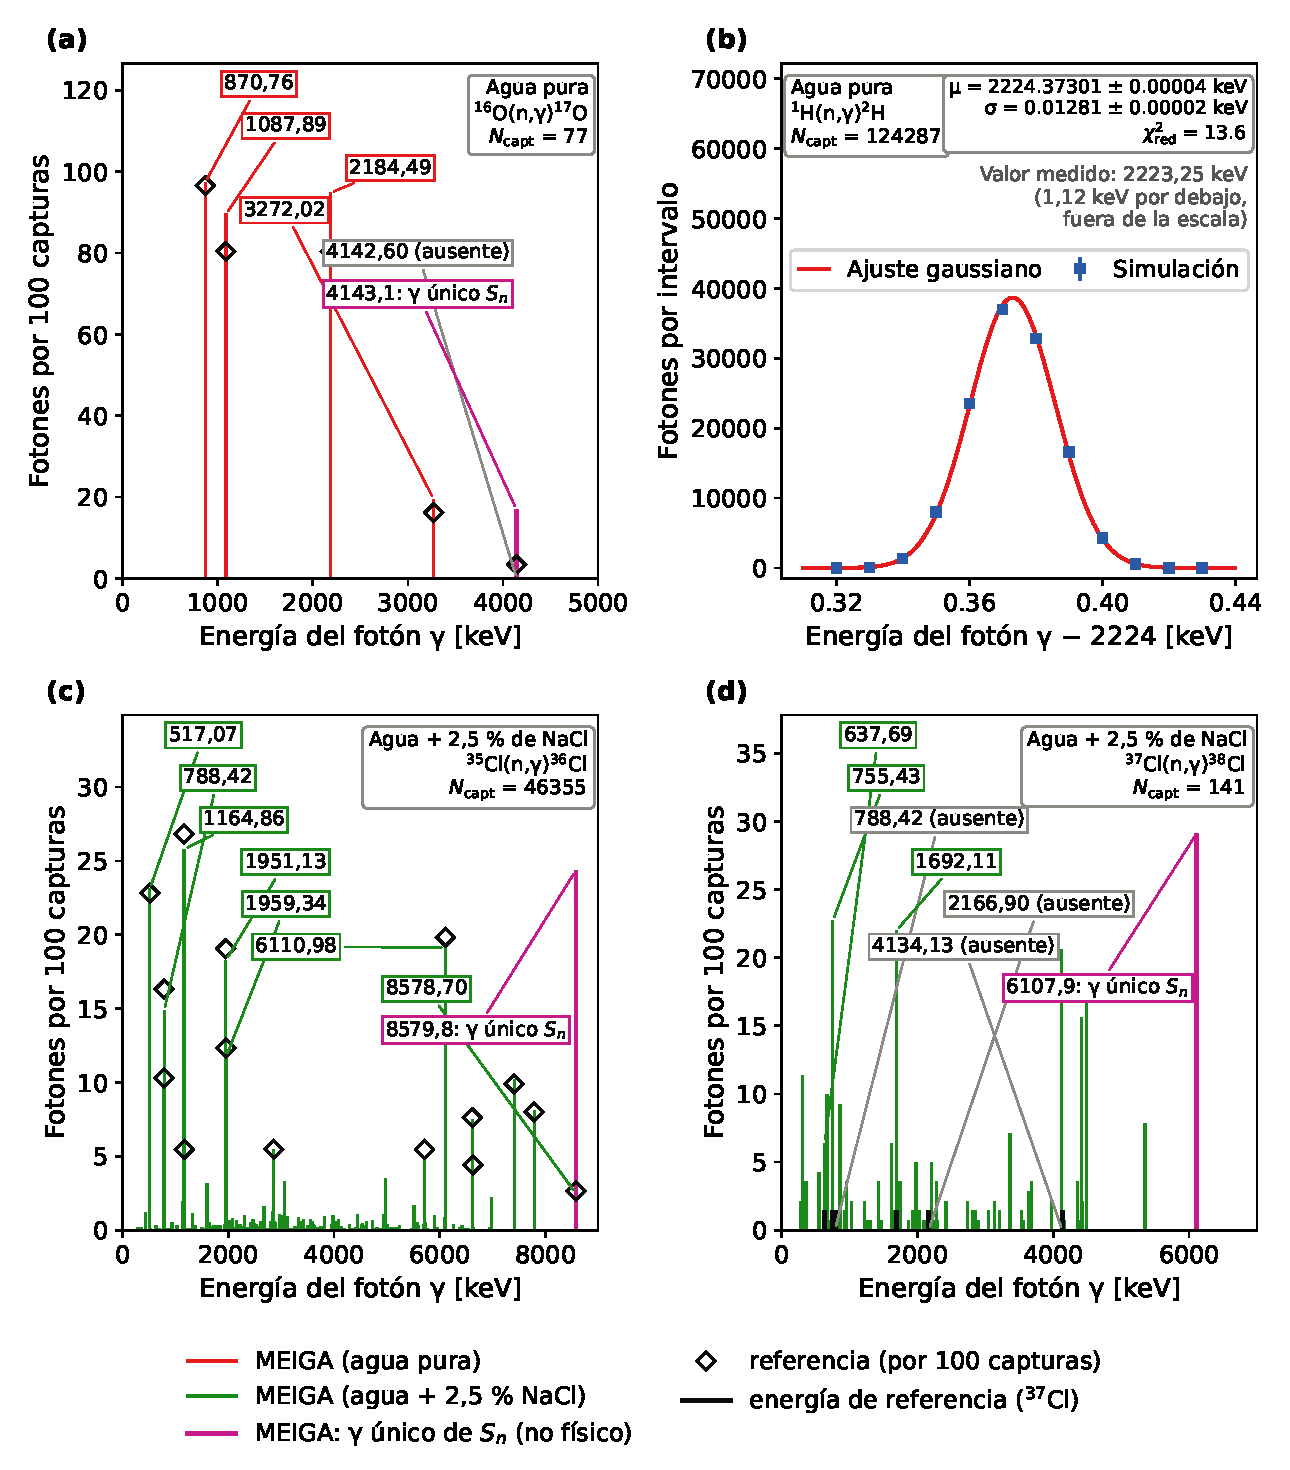
\includegraphics[width=\linewidth]{fig15_espectros_captura_nucleo.pdf}
			\vspace{0.3cm}
			\captionsetup{width=\dimexpr\textwidth+0cm\relax,justification=justified,singlelinecheck=false}
			\caption[Espectros gamma de captura de neutrones en H, O y Cl para un WCD dopado con NaCl]{Espectros gamma producidos por la captura de neutrones en los núcleos presentes en el detector: (a) $^{16}\mathrm{O}(n,\gamma)^{17}\mathrm{O}$ en \textcolor{red}{agua pura}; (b) $^{1}\mathrm{H}(n,\gamma)^{2}\mathrm{H}$ con su ajuste gaussiano; (c) $^{35}\mathrm{Cl}(n,\gamma)^{36}\mathrm{Cl}$ y (d) $^{37}\mathrm{Cl}(n,\gamma)^{38}\mathrm{Cl}$ en \textcolor{green}{agua + 2.5\,\% de NaCl}. Intensidad en fotones por 100 capturas; los rombos indican los valores de referencia \protect\citep{Firestone2016,Nica2012} y las etiquetas, en keV, las energías de la Tabla~\ref{elem-capt-neut}. En magenta se indica el gamma único con toda la energía de separación del neutrón $S_n$ que emite \textsc{Geant4} (véase el texto).}
			\label{fig-lineas-esp-1}
		\end{minipage}
	\end{adjustwidth}
\end{figure}

%----------------------------------------------------------
\paragraph{Captura de neutrones en agua pura:}
%----------------------------------------------------------
En agua pura, la captura radiativa de un neutrón por el hidrógeno,
\begin{equation}
	{}^{1}\mathrm{H}+n \longrightarrow {}^{2}\mathrm{H}+\gamma ,
\end{equation}
produce la línea gamma característica de 2223.25~keV, utilizada por Firestone y R{\'e}vay como línea de referencia para la normalización de sus medidas \citep[Sec.~II.A, Tabla~I, p.~2]{Firestone2016}. Como se observa en la Figura~\ref{fig-lineas-esp-1}(b), el máximo de la distribución simulada se encuentra en
\begin{equation}
	\mu = 2224.373~\mathrm{keV},
\end{equation}
con una dispersión $\sigma \approx 0.013$~keV, del orden de la precisión con que se registran las energías en la salida de la simulación (0.01~keV). La línea simulada está 1.1~keV por encima del valor medido: \textsc{Geant4} emite el gamma con $E_{\gamma}\approx S_{n}(^{2}\mathrm{H})=2224.57$~keV, sin descontar la energía de retroceso del deuterón (1.32~keV; Sec.~\ref{subsubsec:deuterones}). La diferencia es irrelevante para la producción de luz, pero debe tenerse en cuenta al comparar la posición de la línea.

El oxígeno constituye el segundo núcleo del agua que puede capturar neutrones. Para la reacción
\begin{equation}
	{}^{16}\mathrm{O}(n,\gamma){}^{17}\mathrm{O},
\end{equation}
Firestone y R{\'e}vay identifican cinco transiciones principales, con energías de 870.76, 1087.89, 2184.49, 3272.02 y 4142.60~keV \citep[Sec.~II.B.1, Fig.~1, Tabla~III, pp.~2--3]{Firestone2016}, representadas en el esquema de niveles de la Figura~(\ref{trans-oxi-1}). Entre corchetes se indican las intensidades obtenidas en la simulación, que coinciden con las de referencia dentro del error estadístico (190 capturas en $^{16}$O en los cuatro medios). La contribución de la captura en $^{16}$O es considerablemente menor que la del hidrógeno debido a su reducida sección eficaz radiativa térmica,
\begin{equation}
	\sigma_{0}(^{16}\mathrm{O}) = 0.170\pm0.003~\mathrm{mb},
\end{equation}
reportada en la Sec.~II.B.1 \citep[Sec.~II.B.1, p.~3]{Firestone2016}; la transición de 870.76~keV tiene una probabilidad absoluta de emisión $P_{\gamma}=96.6\pm0.5$\,\% y una sección eficaz de producción individual $\sigma_{\gamma}=0.164\pm0.003$~mb.
%, una magnitud distinta de $\sigma_{0}$.

\begin{figure}[!htbp]
	\begin{adjustwidth}{0cm}{0cm}
		\centering
		\begin{minipage}{\linewidth}
			\centering
			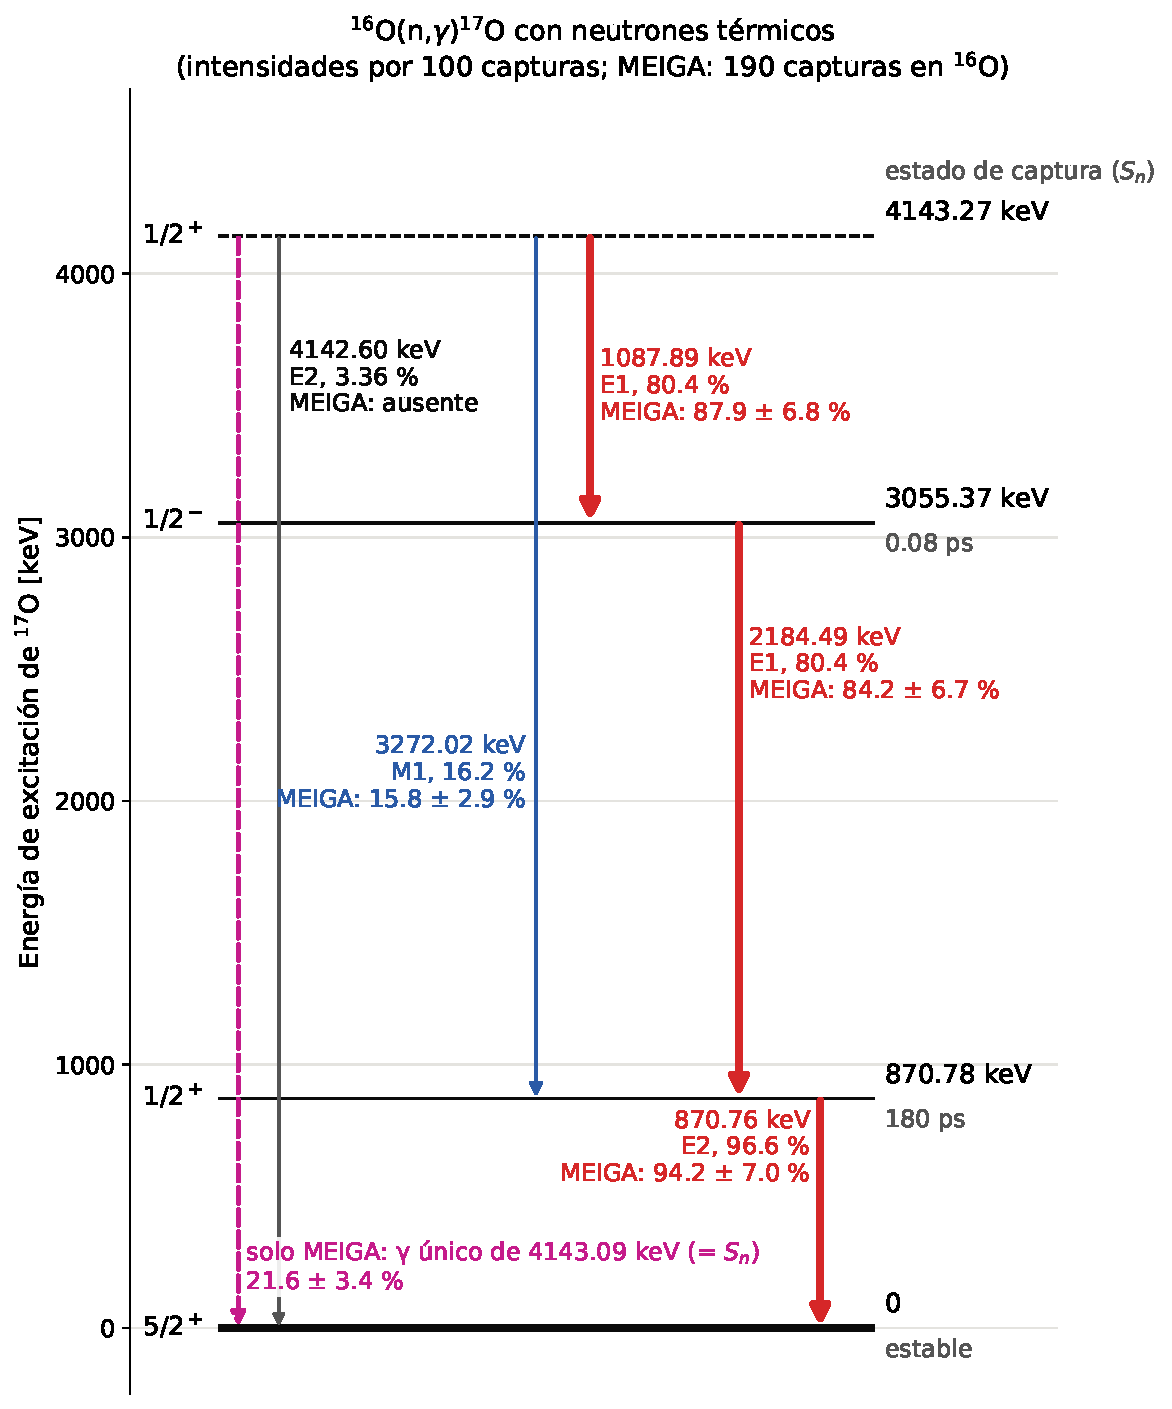
\includegraphics[width=\linewidth]{fig18b_esquema_niveles_O17_MEIGA.pdf}
			\vspace{0.2cm}
			\captionsetup{width=\textwidth,justification=justified,singlelinecheck=false}
			\caption[Esquema de desexcitación gamma tras la captura de neutrones en $^{16}$O]{Esquema de niveles y principales transiciones $\gamma$ de la reacción $^{16}\mathrm{O}(n,\gamma){}^{17}\mathrm{O}$ con neutrones térmicos, elaborado a partir de los datos experimentales de Firestone y R{\'e}vay (Sec.~II.B.1, Fig.~1 y Tabla~III) \protect\citep{Firestone2016} y contrastado con la base CapGam del NNDC \protect\citep{NNDC16OCapGam}. Debajo de cada transición se indica, como «MEIGA», la intensidad por 100 capturas obtenida en la simulación; en magenta, el gamma único de energía $S_n$ que emite \textsc{Geant4}.}
			\label{trans-oxi-1}
		\end{minipage}
	\end{adjustwidth}
\end{figure}

%----------------------------------------------------------
\paragraph{Captura de neutrones en agua dopada con NaCl:}
%----------------------------------------------------------
La incorporación de NaCl introduce canales adicionales de captura. Para los isótopos naturales del cloro,
\begin{equation}
	{}^{35}\mathrm{Cl}+n \longrightarrow {}^{36}\mathrm{Cl}+\gamma , \qquad
	{}^{37}\mathrm{Cl}+n \longrightarrow {}^{38}\mathrm{Cl}+\gamma .
\end{equation}
A diferencia de la captura sobre hidrógeno, caracterizada por una única línea, la captura en $^{35}$Cl libera $Q=8.579$~MeV que se reparten en una cascada de tres a cuatro gammas distribuidos en un intervalo amplio de energías. La Figura~(\ref{fig:esquema-Cl36}) muestra el esquema de niveles de $^{36}$Cl con las quince transiciones más intensas \citep{Nica2012} y, entre corchetes, las intensidades de la simulación en 214\,748 capturas en $^{35}$Cl. Trece de las quince transiciones coinciden con la evaluación dentro de pocos puntos porcentuales, incluidas las primarias de 6110.98~keV (19.4 frente a 19.8 por 100 capturas) y 7414.09~keV (10.0 frente a 9.9) y la transición directa al estado fundamental de 8578.70~keV (2.6 frente a 2.7). Las excepciones son la línea de 1170.94~keV, casi ausente en la simulación (0.5 frente a 5.5), y la de 788.42~keV, algo baja.

% figura girada flotante (paquete rotating): ocupa su propia pagina sin cortar el flujo del texto
\begin{sidewaysfigure}
	\begin{adjustwidth}{0cm}{0cm}
		\centering
		\begin{minipage}{\linewidth}
			\centering
			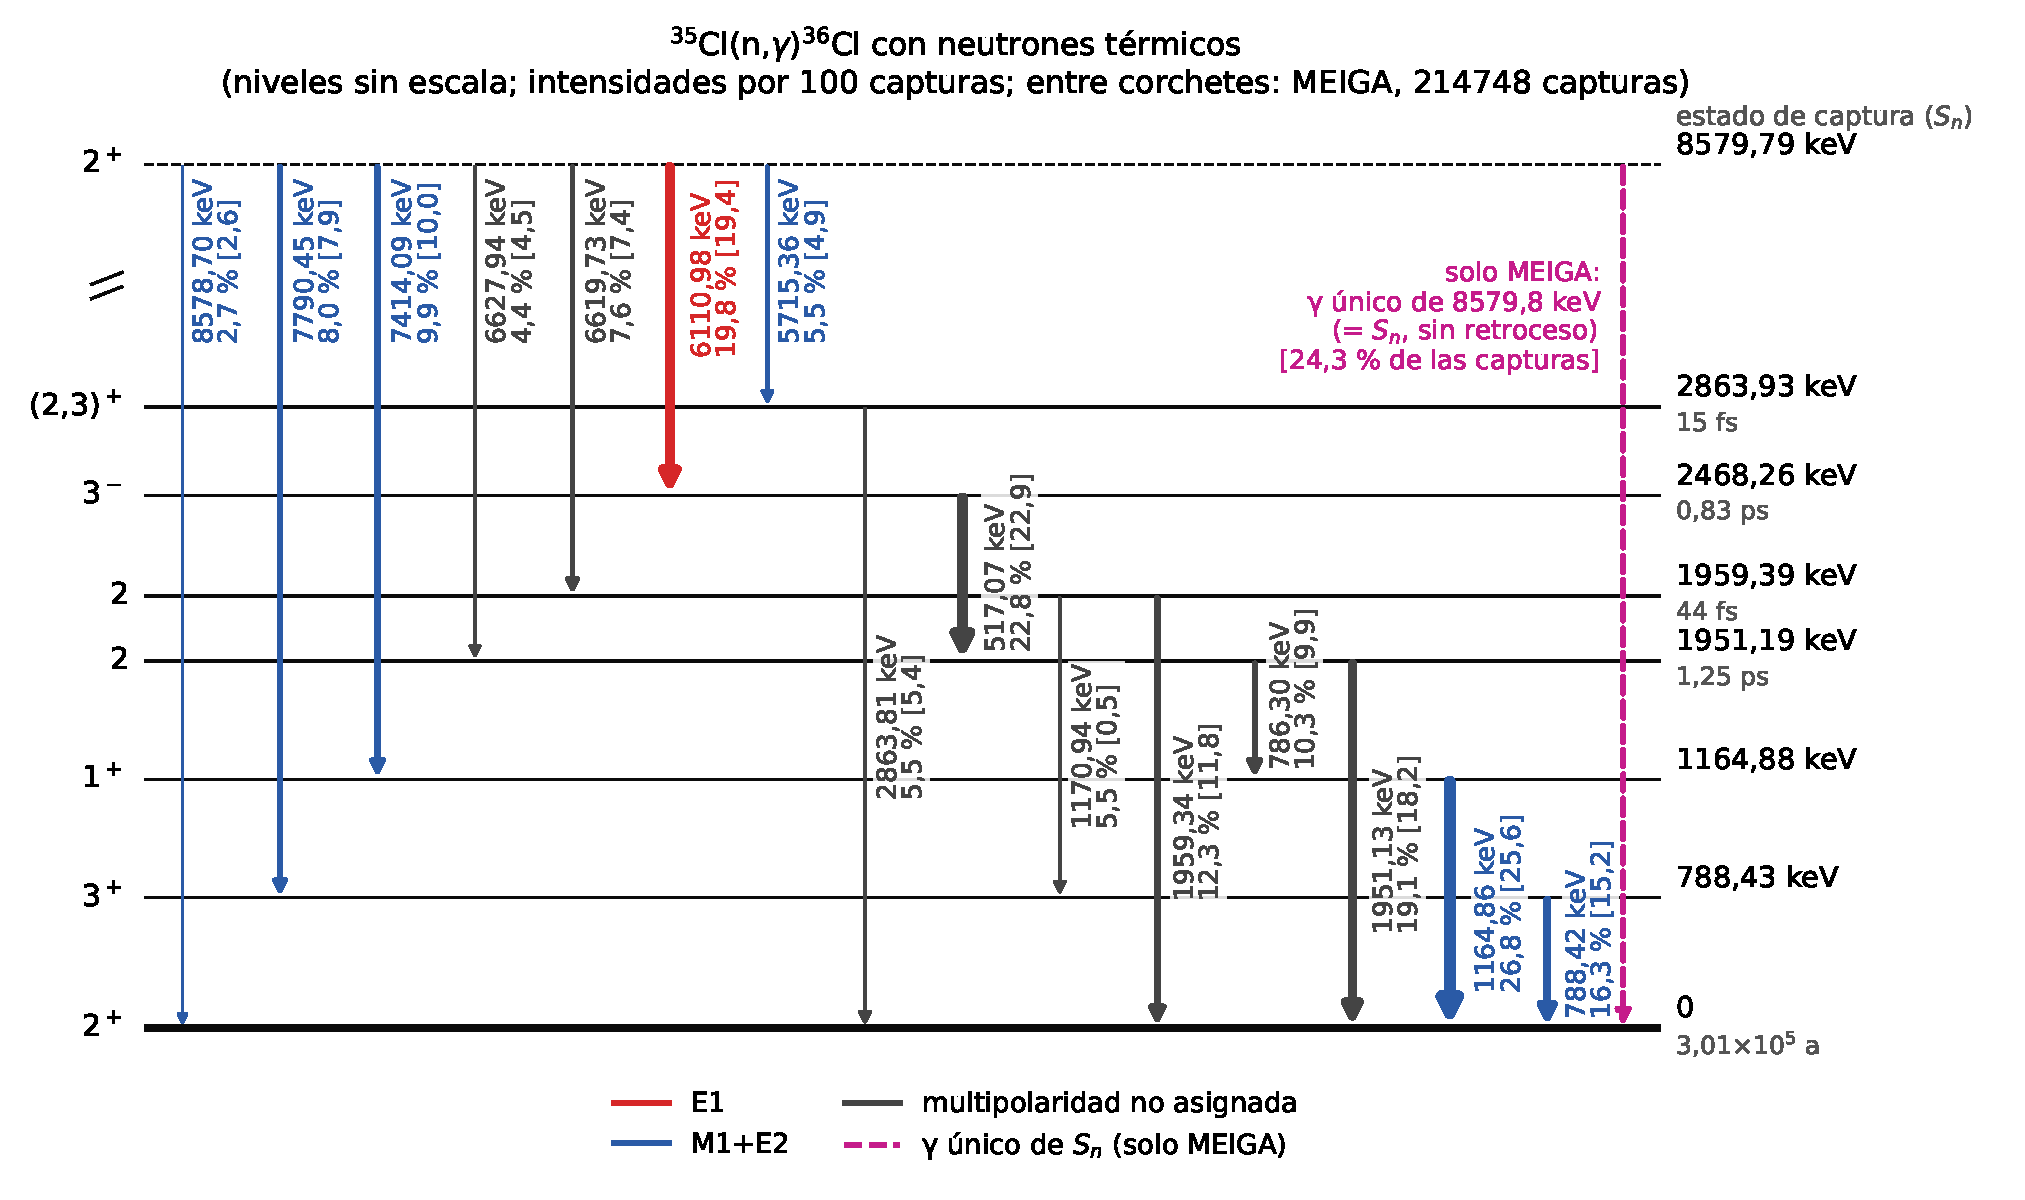
\includegraphics[width=\linewidth,height=0.70\textwidth,keepaspectratio]{fig19b_esquema_niveles_Cl36_MEIGA.pdf}
			\vspace{0.2cm}
			\captionsetup{width=\textwidth,justification=justified,singlelinecheck=false}
			\caption[Esquema de desexcitación gamma tras la captura de neutrones en $^{35}$Cl]{Esquema de niveles de $^{36}$Cl y transiciones $\gamma$ más intensas de la captura $^{35}\mathrm{Cl}(n,\gamma)^{36}\mathrm{Cl}$ con neutrones térmicos (evaluación ENSDF \protect\citep{Nica2012}; niveles sin escala). Intensidades por 100 capturas según la evaluación; entre corchetes, los valores de la simulación (214\,748 capturas en $^{35}$Cl). En magenta, el gamma único de energía $S_n$ que emite \textsc{Geant4}.}
			\label{fig:esquema-Cl36}
		\end{minipage}
	\end{adjustwidth}
\end{sidewaysfigure}

La Tabla~(\ref{elem-capt-neut}) reúne los parámetros nucleares de los isótopos del volumen activo, las energías de las líneas de captura y la línea correspondiente en la simulación. Respecto a la versión anterior de esta tabla se unificaron las energías con las de los esquemas de niveles: las del $^{16}$O siguen ahora a Firestone y R{\'e}vay (Fig.~1), y el valor de 1959.13~keV del $^{35}$Cl, que mezclaba dos líneas reales, se separó en 1951.13 y 1959.34~keV.

\begin{table}[!htbp]
	\captionsetup{width=\linewidth,justification=justified,singlelinecheck=false}
	\caption[Parámetros nucleares de los isótopos presentes en el volumen detector]{Parámetros nucleares de los principales isótopos del volumen activo y energías de las líneas $\gamma$ de captura de neutrones térmicos, contrastadas con la base CapGam del NNDC \protect\citep{NNDC16OCapGam}, con Firestone y R{\'e}vay para $^{16}$O \protect\citep[Sec.~II.B.1, Tabla~III]{Firestone2016} y con la evaluación ENSDF para $^{35}$Cl \protect\citep{Nica2012}. La última columna da la misma transición en la simulación y su intensidad por 100 capturas en ese isótopo (capturas en el agua de los cuatro medios: $^{1}$H: 316\,177; $^{16}$O: 190; $^{35}$Cl: 214\,748; $^{23}$Na: 3\,483; $^{37}$Cl: 707). $\sigma_{0}$ es la sección eficaz total de captura radiativa térmica del isótopo y no la de producción de cada línea. En magenta, el gamma único con toda la energía de separación que emite \textsc{Geant4}, sin equivalente en la naturaleza.}
	\label{elem-capt-neut}
	\centering
	\renewcommand{\arraystretch}{1.3}
	\setlength{\tabcolsep}{3pt}
	\small
	\begin{tabularx}{\linewidth}{>{\centering\arraybackslash}p{0.11\linewidth} >{\centering\arraybackslash}X >{\centering\arraybackslash}p{0.19\linewidth} >{\raggedleft\arraybackslash}p{0.14\linewidth} >{\raggedleft\arraybackslash}p{0.27\linewidth}}
		\toprule
		\multicolumn{5}{c}{\textbf{Parámetros nucleares y líneas $\gamma$ de captura}}\\
		\midrule
		\textbf{Isótopo} & \textbf{\makecell{Abundancia\\isotópica (\%)}} & \textbf{$\sigma_{0}$ (mb)} & \textbf{$E_{\gamma}$ (keV)} & \textbf{\makecell{Simulación: $E_{\gamma}$ (keV)\\(por 100 capturas)}}\\
		\midrule
		\rowcolor{gray!18}$^{1}$H & 99.99 & $332.60 \pm 0.70$ & 2223.25 & 2224.37 \;(100.0\,\%) \\
		\midrule
		$^{16}$O & 99.76 & $0.170 \pm 0.003$ & 870.76 & 870.80 \;(94.2\,\%) \\
		 & & & 1087.89 & 1088.00 \;(87.9\,\%) \\
		 & & & 2184.49 & 2184.20 \;(84.7\,\%) \\
		 & & & 3272.02 & 3272.20 \;(15.8\,\%) \\
		 & & & 4142.60 & -- \\
		 & \multicolumn{3}{r}{\textcolor{magenta!70!black}{$\gamma$ único de $S_n$ (solo \textsc{Geant4})}} & \textcolor{magenta!70!black}{4143.09 \;(21.6\,\%)} \\
		\midrule
		\rowcolor{gray!18}$^{35}$Cl & 75.78 & $43840 \pm 170$ & 517.07 & 517.08 \;(22.9\,\%) \\
		\rowcolor{gray!18} & & & 788.42 & 788.43 \;(15.2\,\%) \\
		\rowcolor{gray!18} & & & 1164.86 & 1164.87 \;(25.6\,\%) \\
		\rowcolor{gray!18} & & & 1951.13 & 1951.14 \;(18.2\,\%) \\
		\rowcolor{gray!18} & & & 1959.34 & 1959.36 \;(11.8\,\%) \\
		\rowcolor{gray!18} & & & 6110.98 & 6110.85 \;(19.4\,\%) \\
		\rowcolor{gray!18} & & & 8578.70 & 8578.59 \;(2.6\,\%) \\
		\rowcolor{gray!18} & \multicolumn{3}{r}{\textcolor{magenta!70!black}{$\gamma$ único de $S_n$ (solo \textsc{Geant4})}} & \textcolor{magenta!70!black}{8579.81 \;(24.3\,\%)} \\
		\midrule
		$^{23}$Na & 100 & $527 \pm 7$ & 472.20 & 472.26 \;(0.6\,\%) \\
		 & \multicolumn{3}{r}{\textcolor{magenta!70!black}{$\gamma$ único de $S_n$ (solo \textsc{Geant4})}} & \textcolor{magenta!70!black}{6959.44 \;(11.4\,\%)} \\
		\midrule
		\rowcolor{gray!18}$^{37}$Cl & 24.22 & $553 \pm 17$ & 637.69 & 637.50 \;(11.5\,\%) \\
		\rowcolor{gray!18} & & & 755.43 & 755.47 \;(26.0\,\%) \\
		\rowcolor{gray!18} & & & 788.42 & -- \\
		\rowcolor{gray!18} & & & 1692.11 & 1692.15 \;(19.9\,\%) \\
		\rowcolor{gray!18} & & & 2166.90 & -- \\
		\rowcolor{gray!18} & & & 4134.13 & -- \\
		\rowcolor{gray!18} & \multicolumn{3}{r}{\textcolor{magenta!70!black}{$\gamma$ único de $S_n$ (solo \textsc{Geant4})}} & \textcolor{magenta!70!black}{6107.88 \;(28.1\,\%)} \\
		\bottomrule
	\end{tabularx}
\end{table}

\paragraph{Limitación del modelo de captura de Geant4:} Además de las transiciones reales, \textsc{Geant4} emite en el 24.3\,\% de las capturas en $^{35}$Cl un único gamma de 8579.8~keV, igual a $S_{n}$ sin la corrección por retroceso del núcleo, distinto de la transición real al estado fundamental (8578.70~keV, 2.7\,\%, bien reproducida). El mismo comportamiento aparece en el $^{16}$O (21.6\,\% de las capturas con un único gamma de 4143.09~keV, mientras que la transición real de 4142.60~keV no aparece), en el $^{37}$Cl (28\,\%) y en el $^{23}$Na (11\,\%), cuya línea de 472.20~keV prácticamente no se produce. Que la fracción sea similar en núcleos distintos indica que el origen está en el código de captura de alta precisión (\texttt{G4NeutronHP}) y no en los datos nucleares. En el resto de las capturas los gammas de la cascada se sortean de forma independiente a partir de las tablas de producción de fotones de la evaluación, sin imponer la conservación de la energía en cada captura (Figura~\ref{fig:cascadas-cl}): las 46\,355 capturas en $^{35}$Cl del medio con 2.5\,\% de NaCl emiten en promedio 2.80 gammas con una energía total media de 10.14~MeV (percentiles 5--95: 2.8--20.9~MeV), en lugar de 8.579~MeV; solo el 26\,\% de las cascadas suma $Q$ dentro del 1\,\%. Estos valores son los mismos en los tres medios con NaCl (10.12--10.14~MeV en promedio), como corresponde a una propiedad del modelo y no del medio. Las intensidades por captura de las líneas coinciden con la evaluación, pero la energía emitida por captura no se conserva. \textsc{Geant4} permite usar en su lugar \texttt{G4PhotonEvaporation}, que genera cascadas que sí conservan la energía (variable de entorno \texttt{G4NEUTRONHP\_USE\_ONLY\_PHOTONEVAPORATION}).

\begin{figure}[!htbp]
	\begin{adjustwidth}{0cm}{0cm}
		\centering
		\begin{minipage}{\linewidth}
			\centering
			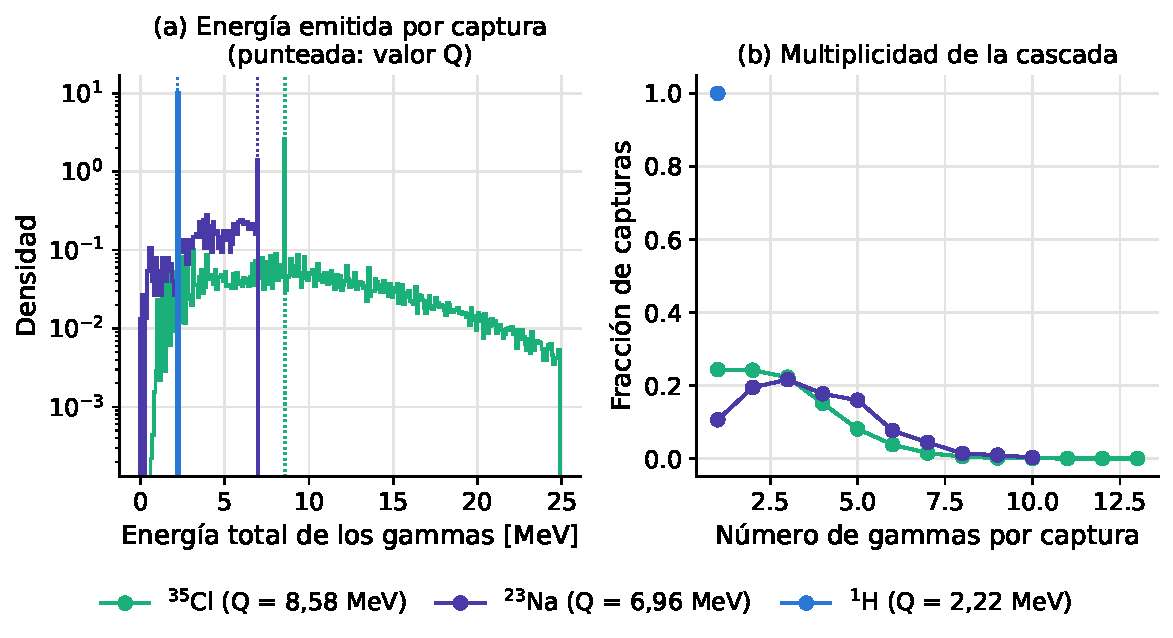
\includegraphics[width=\linewidth]{fig12_cascadas_cloro_nacl25.pdf}
			\vspace{0.2cm}
			\captionsetup{width=\textwidth,justification=justified,singlelinecheck=false}
			\caption[Energía total y multiplicidad de las cascadas de captura]{Energía total emitida por captura y multiplicidad de la cascada gamma en $^{35}$Cl, $^{23}$Na y $^{1}$H en \textcolor{green}{agua + 2.5\,\% de NaCl}. La línea vertical indica la energía de separación del neutrón, $Q=8.579$~MeV, en $^{36}$Cl.}
			\label{fig:cascadas-cl}
		\end{minipage}
	\end{adjustwidth}
\end{figure}

\paragraph{Implicaciones para la respuesta Cherenkov del WCD:} La cadena de procesos que conduce de la captura a la señal es
\begin{gather}
	n + {}^{A}\mathrm{X} \longrightarrow {}^{A+1}\mathrm{X}^{*} \longrightarrow {}^{A+1}\mathrm{X} + \sum_{k}\gamma_{k}, \\
	\gamma_{k} + e^{-}_{\mathrm{at}} \longrightarrow e^{-} \;(\text{Compton, fotoeléctrico, pares}) \longrightarrow \gamma_{\mathrm{Ch}} .
\end{gather}
La energía gamma de captura por neutrón incidente pasa de 1.85~MeV en \textcolor{red}{agua pura} a 4.39~MeV (\textcolor{green}{2.5\,\%}), 5.71~MeV (\textcolor{violet}{5\,\%}) y 7.40~MeV (\textcolor{orange}{10\,\%}), es decir, se multiplica por 2.4, 3.1 y 4.0 (Tabla~\ref{tab:efecto-nacl-captura}). Este es el origen del aumento de la luz Cherenkov con la concentración de NaCl. Debido a la limitación descrita, en los medios con NaCl la energía de las capturas en Cl está sobreestimada en promedio en un 18\,\%, lo que afecta a la escala absoluta de la luz y de la carga de esos medios, aunque no al signo de las tendencias.

%==========================================================
\section{Comparación de los espectros de fotones gamma generados por captura de neutrones}
\label{subsubsec:espectros-gamma}
%==========================================================

\noindent La Figura~(\ref{fig:comparacion-espectros-gamma-1}) compara los espectros de energía de los fotones $\gamma$ creados en el agua después de la interacción de neutrones monocromáticos de 500~MeV. La subfigura (a) corresponde al espectro reportado por \citet[Fig.~3, pp.~2219--2220]{Sidelnik2020}; la subfigura (b), al espectro obtenido en este trabajo con el mismo formato.

\begin{figure}[!htbp]
	\centering
	\includegraphics[width=\linewidth]{espectro-gamma-ivan.png}\par
	\vspace{0.15cm}
	{\normalsize\bfseries (a) Trabajo previo}\par
	{\small Sidelnik \textit{et al.} (2020)}\par
	\vspace{0.2cm}
	\captionsetup{width=\linewidth,justification=justified,singlelinecheck=false}
	\caption[Comparación entre los espectros de radiación gamma por captura de neutrones]{Comparación entre los espectros de radiación $\gamma$ creados en el agua por neutrones de 500~MeV. (a) Fig.~3 de \protect\citet{Sidelnik2020} para \textcolor{red}{agua pura} (\textcolor{red}{rojo}), agua + 2.5\,\% de NaCl (\textcolor{green}{verde}), agua + 5\,\% de NaCl (\textcolor{violet}{violeta}) y agua + 10\,\% de NaCl (\textcolor{orange}{naranja}). (b) Presente trabajo en \textcolor{red}{agua pura}: espectro con el mismo formato, comparación con la curva digitalizada con el pico de 2.223~MeV igualado, composición por proceso creador y cocientes de líneas.}
	\label{fig:comparacion-espectros-gamma-1}
\end{figure}

\begin{figure}[!htbp]
	\ContinuedFloat
	\centering
	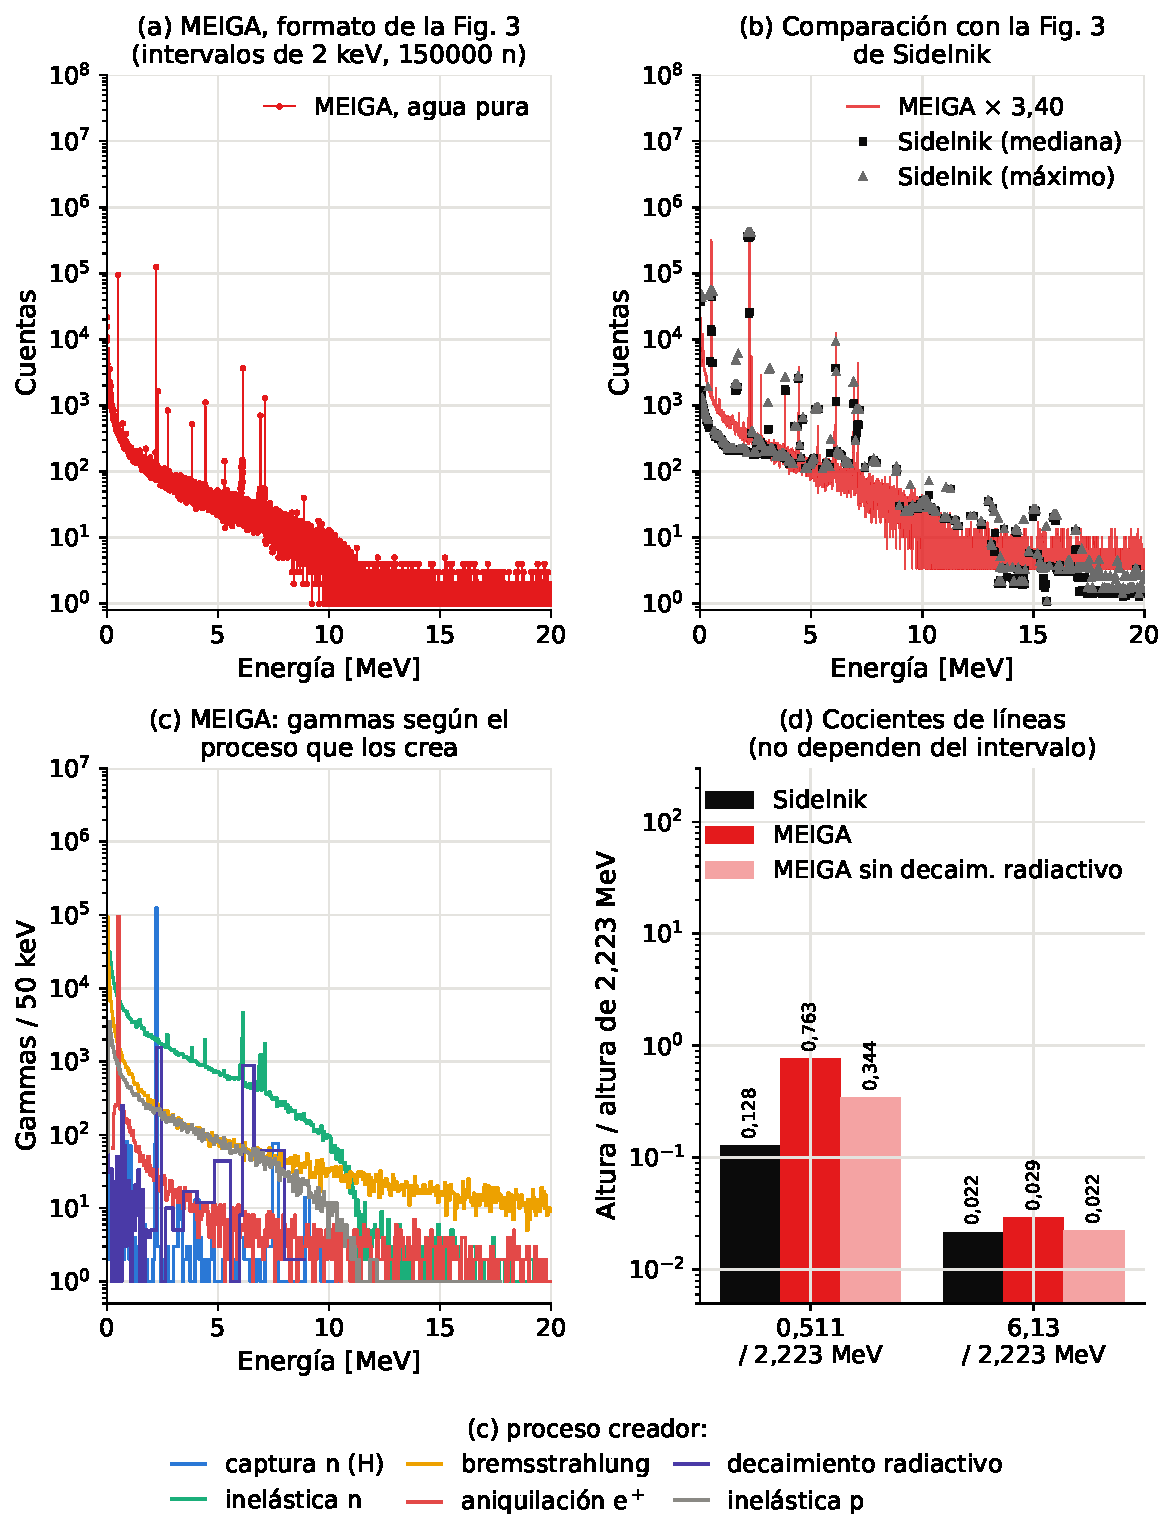
\includegraphics[width=\linewidth]{fig11_espectro_gamma_tipo_sidelnik.pdf}\par
	\vspace{0.15cm}
	{\normalsize\bfseries (b) Presente trabajo}\par
	{\small Reproducción realizada en esta investigación}\par
	\vspace{0.2cm}
	\captionsetup{width=\linewidth,justification=justified,singlelinecheck=false}
	\caption[]{(Continuación) (b) Presente trabajo; véase la descripción en la parte (a) de esta figura.}
\end{figure}

\paragraph{Normalización:} El eje vertical de la Fig.~3 del trabajo de referencia está en unidades arbitrarias: su línea de 2.223~MeV contiene unas $4.2\times10^{5}$ cuentas, más que el número de neutrones simulados ($1.5\times10^{5}$). En la presente simulación la línea contiene 124\,397 cuentas, una por captura en H. Por ello la comparación se realiza con magnitudes que no dependen de la normalización: cocientes entre alturas de líneas y la forma del continuo con el pico de 2.223~MeV igualado. Con bines de 2~keV el cociente pico/continuo entre 3 y 5~MeV (1\,777--3\,659) coincide con el del artículo (1\,946--3\,075).

La Tabla~(\ref{tab:gammas-creados}) resume la producción de gammas y de electrones en el agua. La Tabla~(\ref{tab:cocientes-lineas}) compara los cocientes de las líneas principales en \textcolor{red}{agua pura}.

\begin{table}[!htbp]
	\centering
	\small
	\captionsetup{width=\linewidth,justification=justified,singlelinecheck=false}
	\caption[Gammas y electrones creados en el agua por neutrón incidente]{Gammas y electrones creados dentro del agua por neutrón incidente de 500~MeV.}
	\label{tab:gammas-creados}
	\renewcommand{\arraystretch}{1.15}
	\resizebox{\textwidth}{!}{\begin{tabular}{lcccc}
		\toprule
		 & \textcolor{red}{\textbf{Agua pura}} & \textcolor{green}{\textbf{2.5\,\% NaCl}} & \textcolor{violet}{\textbf{5\,\% NaCl}} & \textcolor{orange}{\textbf{10\,\% NaCl}} \\
		\midrule
		Gammas creados en el agua & 5.98 & 7.03 & 7.68 & 8.65 \\
		\quad de inelásticas de neutrones & 2.63 & 2.70 & 2.77 & 2.93 \\
		\quad de captura & 0.83 & 1.43 & 1.76 & 2.19 \\
		\quad de bremsstrahlung / aniquilación & 1.23 / 0.67 & 1.42 / 0.76 & 1.56 / 0.82 & 1.74 / 0.90 \\
		Energía gamma de captura (MeV) & 1.855 & 4.393 & 5.713 & 7.404 \\
		e$^{\pm}$ creados por gammas & 44.1 & 51.4 & 55.8 & 62.2 \\
		\quad Compton / fotoeléctrico & 37.1 / 6.80 & 41.4 / 9.57 & 43.6 / 11.74 & 46.3 / 15.25 \\
		\quad fracción sobre el umbral Cherenkov (0.264~MeV) & 8.0\,\% & 8.3\,\% & 8.5\,\% & 8.7\,\% \\
		\bottomrule
	\end{tabular}}
\end{table}

\begin{table}[!htbp]
	\centering
	\small
	\captionsetup{width=\linewidth,justification=justified,singlelinecheck=false}
	\caption[Cocientes entre las alturas de las líneas gamma principales]{Cocientes entre las alturas de las líneas gamma principales en \textcolor{red}{agua pura}. $^{*}$Estimado restando la fracción de positrones procedentes de desintegraciones $\beta^{+}$ de larga vida.}
	\label{tab:cocientes-lineas}
	\renewcommand{\arraystretch}{1.15}
	\begin{tabular}{lccc}
		\toprule
		\textbf{Cociente de alturas} & \textbf{Sidelnik et al.} & \textbf{Este trabajo} & \textbf{\makecell{Este trabajo, sin\\decaimiento radiactivo}} \\
		\midrule
		0.511~MeV / 2.223~MeV & 0.128 & 0.763 & 0.344$^{*}$ \\
		6.13~MeV / 2.223~MeV & 0.022 & 0.029 & 0.022 \\
		\bottomrule
	\end{tabular}
\end{table}

\paragraph{Líneas de 2.223 y 6.13~MeV:} La línea de 6.13~MeV del $^{16}$O la producen la dispersión inelástica de neutrones y la desintegración del $^{16}$N ($T_{1/2}=7.1$~s), producido por la reacción $^{16}\mathrm{O}(n,p)$. Sin esta última, el cociente con la línea de captura en H es 0.022, igual al del trabajo de referencia: la captura en H y la dispersión inelástica en O se reproducen con la misma proporción.

\paragraph{Línea de aniquilación (0.511~MeV):} En la presente simulación es unas seis veces más intensa, relativa a la línea de 2.223~MeV, que en el trabajo de referencia. Los positrones que la producen proceden de desintegraciones $\beta^{+}$ de núcleos de espalación del oxígeno ($^{15}$O, $^{13}$N y $^{11}$C, con vidas medias de minutos; 55\,\%), de la conversión de gammas de alta energía en pares (39\,\%) y de la desintegración de muones positivos procedentes de $\pi^{+}$ (6\,\%). \textsc{Geant4} simula las desintegraciones radiactivas sin límite de tiempo; sin ellas, el cociente bajaría a 0.34, y el exceso restante es coherente con la mayor producción de piones discutida en la Sec.~\ref{subsubsec:cherenkov}.

\paragraph{Continuo:} Entre 2.5 y 9~MeV la forma del continuo coincide con la del trabajo de referencia (cola de la dispersión inelástica de neutrones). Por debajo de 1.5~MeV el continuo simulado es varias veces más alto, dominado por el bremsstrahlung de electrones y positrones de alta energía asociados a la producción de piones.

\paragraph{Líneas del cloro:} La Tabla~(\ref{tab:lineas-cl}) compara las alturas de las líneas respecto a la de 2.223~MeV en los medios con NaCl. Las líneas de la cascada del $^{36}$Cl de 1.165, 6.11, 7.41 y 7.79~MeV coinciden con el trabajo de referencia dentro del 2--10\,\% en las tres concentraciones: la proporción de capturas en Cl respecto a H y la intensidad de esas transiciones son las mismas en las dos simulaciones. Las diferencias se concentran en la línea de 0.511~MeV, por las causas ya descritas, y en la de 8.58~MeV, unas diez veces más intensa en este trabajo por el gamma único de $S_n$ de \textsc{Geant4}.

\begin{table}[!htbp]
	\centering
	\small
	\captionsetup{width=\linewidth,justification=justified,singlelinecheck=false}
	\caption[Altura de las líneas del cloro respecto a la línea de 2.223~MeV]{Altura de las líneas gamma respecto a la de 2.223~MeV en los medios con NaCl, frente a la Fig.~3 de \protect\citet{Sidelnik2020} digitalizada. La digitalización (25.6~keV por píxel) no separa las líneas de 0.511/0.517~MeV ni las de 6.11/6.13~MeV.}
	\label{tab:lineas-cl}
	\renewcommand{\arraystretch}{1.15}
	\resizebox{\textwidth}{!}{\begin{tabular}{lcccccc}
		\toprule
		 & \multicolumn{2}{c}{\textcolor{green}{\textbf{2.5\,\% NaCl}}} & \multicolumn{2}{c}{\textcolor{violet}{\textbf{5\,\% NaCl}}} & \multicolumn{2}{c}{\textcolor{orange}{\textbf{10\,\% NaCl}}} \\
		\cmidrule(lr){2-3}\cmidrule(lr){4-5}\cmidrule(lr){6-7}
		\textbf{Línea (MeV) / 2.223~MeV} & \textbf{Sidelnik} & \textbf{Este trabajo} & \textbf{Sidelnik} & \textbf{Este trabajo} & \textbf{Sidelnik} & \textbf{Este trabajo} \\
		\midrule
		0.511 / 0.517 & 0.423 & 1.305 & 0.678 & 1.788 & 1.181 & 2.796 \\
		1.165 (Cl) & 0.165 & 0.147 & 0.312 & 0.277 & 0.574 & 0.561 \\
		1.951 (Cl) & 0.179 & 0.104 & 0.339 & 0.200 & 0.624 & 0.397 \\
		6.11 / 6.13 & 0.115 & 0.109 & 0.217 & 0.212 & 0.412 & 0.425 \\
		7.41 (Cl) & 0.059 & 0.057 & 0.112 & 0.107 & 0.206 & 0.216 \\
		7.79 (Cl) & 0.047 & 0.046 & 0.089 & 0.084 & 0.165 & 0.172 \\
		8.58 (Cl) & 0.016 & 0.151 & 0.029 & 0.292 & 0.054 & 0.583 \\
		\bottomrule
	\end{tabular}}
\end{table}

La Figura~(\ref{fig:espectro-gamma-nacl25}) muestra el espectro gamma completo en \textcolor{green}{agua + 2.5\,\% de NaCl}, con el mismo formato y los mismos cuatro paneles que el del \textcolor{red}{agua pura} (Figura~\ref{fig:comparacion-espectros-gamma-1}). Respecto al agua pura aparecen las líneas de la cascada del $^{36}$Cl entre 0.5 y 8.58~MeV (panel a), y la componente de captura ya no se limita a la línea de 2.223~MeV del H, sino que se extiende hasta la energía de separación del neutrón en $^{36}$Cl (panel c); el resto de las componentes (inelásticas de neutrones y protones, bremsstrahlung, aniquilación y decaimiento radiactivo) no cambia con la sal. Para la comparación con la curva digitalizada se iguala de nuevo el pico de 2.223~MeV (panel b); el factor necesario, 3.38, es prácticamente el mismo que en agua pura (3.40), lo que confirma que se trata de la normalización arbitraria del eje del artículo y no de una diferencia física. Con ese factor, las líneas del Cl aparecen en las mismas energías y con alturas relativas comparables; entre 2.5 y 9~MeV la curva digitalizada queda algo por encima del continuo simulado, porque a la resolución de la digitalización (25.6~keV por píxel) las numerosas líneas del Cl se confunden con el continuo. Por encima de 10~MeV ambos espectros quedan en el nivel de unas pocas cuentas. El panel (d) resume los cocientes de la Tabla~(\ref{tab:lineas-cl}): las líneas de 1.165, 6.11, 7.41 y 7.79~MeV coinciden con el artículo dentro del 2--10\,\%, la de 1.951~MeV queda por debajo porque en la figura del artículo se superpone con la de 1.959~MeV, la de 0.511~MeV es unas tres veces más intensa por los emisores $\beta^{+}$ de larga vida y los piones, y la de 8.58~MeV es unas diez veces más intensa por el gamma único de $S_n$ que emite \textsc{Geant4}. Los espectros de 5 y 10\,\% de NaCl tienen la misma estructura y escalan con la fracción de capturas en Cl.

\begin{figure}[!htbp]
	\centering
	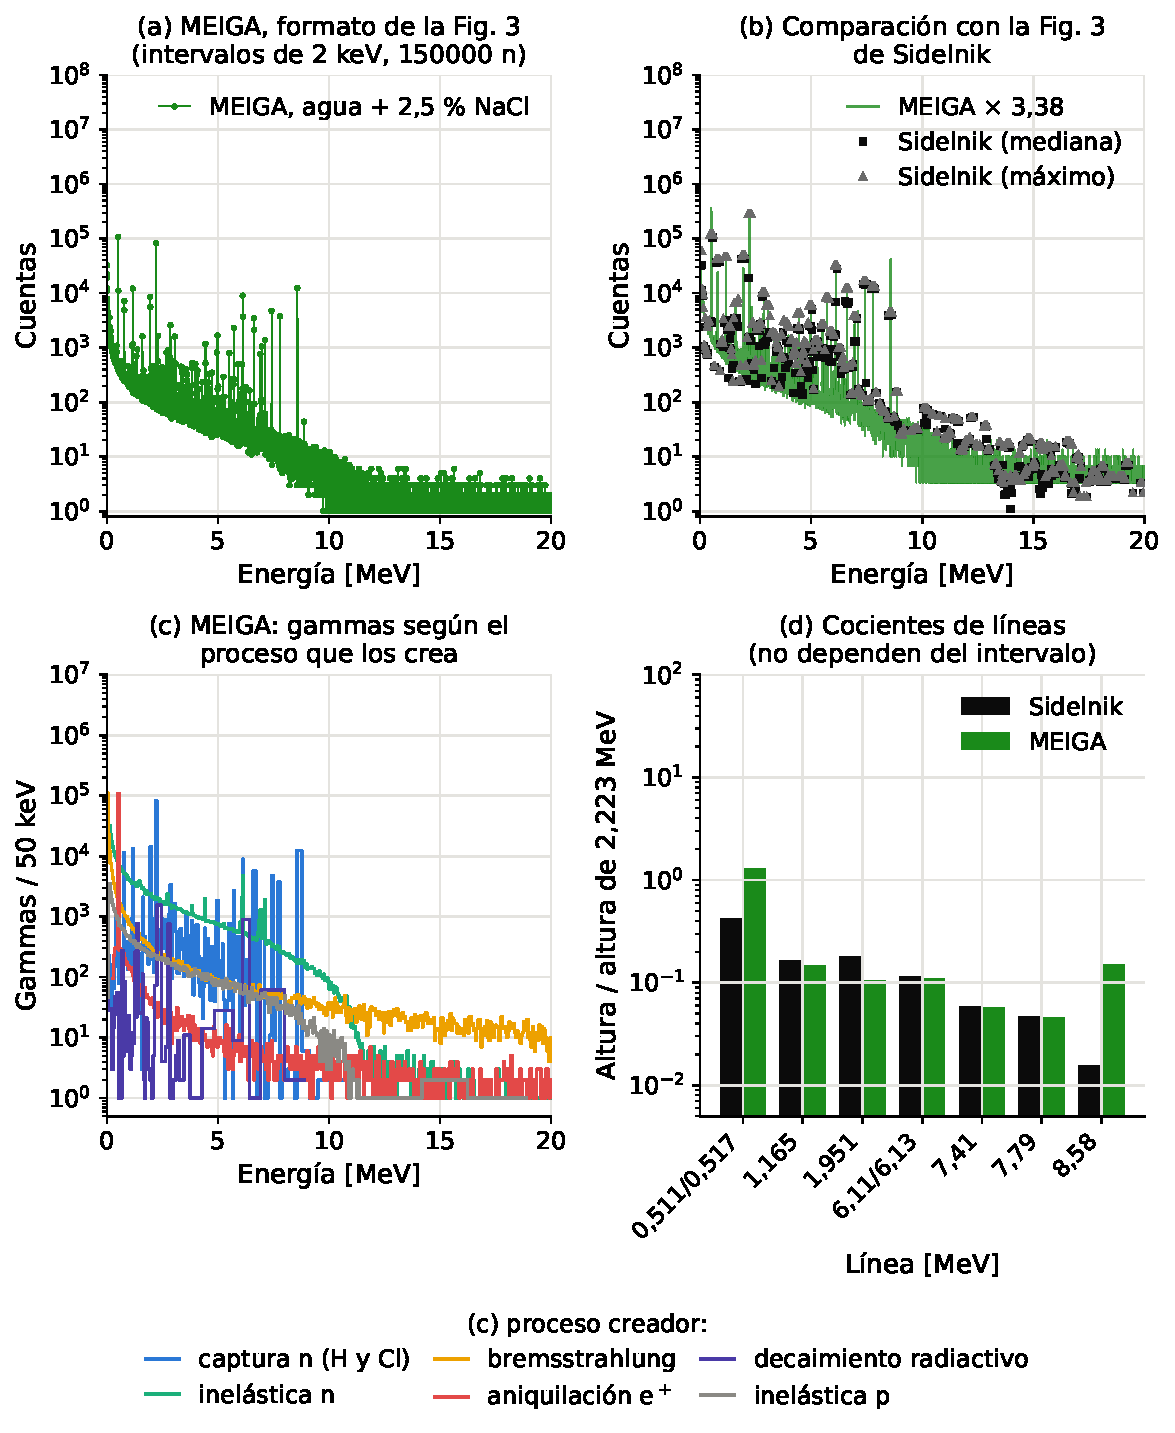
\includegraphics[width=\linewidth]{fig11_espectro_gamma_tipo_sidelnik_nacl25.pdf}
	\vspace{0.2cm}
	\captionsetup{width=\textwidth,justification=justified,singlelinecheck=false}
	\caption[Espectro gamma en agua + 2.5\,\% de NaCl frente a la Fig.~3 de Sidelnik et al.]{Espectro de energía de los gammas creados en \textcolor{green}{agua + 2.5\,\% de NaCl} por neutrones de 500~MeV: (a) formato de la Fig.~3 de \protect\citet{Sidelnik2020} (intervalos de 2~keV, $1.5\times10^{5}$ neutrones); (b) comparación con la curva digitalizada del artículo, con el pico de 2.223~MeV igualado; (c) composición por proceso creador; (d) cocientes de las alturas de las líneas principales respecto a la de 2.223~MeV (Tabla~\ref{tab:lineas-cl}).}
	\label{fig:espectro-gamma-nacl25}
\end{figure}

\paragraph{Espectro acumulado:} \citet[Fig.~4, p.~2220]{Sidelnik2020} presentan los mismos gammas acumulados de derecha a izquierda, $N(\geq E)$. La Figura~(\ref{gama-esp}) muestra el espectro completo de los cuatro medios y su acumulado, y la Figura~(\ref{fig:gammas-acumulados}) la comparación con la Fig.~4 digitalizada. Tres cocientes, independientes de la normalización, resumen la comparación:
\begin{itemize}
	\item \textbf{Línea de 2.223~MeV frente a los gammas de más de 3~MeV}, $[N(\geq2)-N(\geq3)]/N(\geq3)$: 2.32 en el artículo y 1.27 en este trabajo. Por cada captura en H, la presente simulación produce $\approx$\,1.6--1.8 veces más gammas de desexcitación nuclear tras la dispersión inelástica de neutrones, conclusión que coincide con la obtenida del espectro de electrones (Sec.~\ref{subsubsec:electrones}).
	\item \textbf{Gammas de más de 20~MeV}, $N(\geq20)/N(\geq3)$: 0.029 en el artículo, 0.163 en este trabajo y 0.0031 sin los eventos con piones. Los gammas de alta energía proceden casi exclusivamente de los piones ($\pi^{0}\to\gamma\gamma$ y bremsstrahlung de sus cascadas); el trabajo de referencia queda entre las dos curvas, con unas seis veces menos piones en este observable.
	\item \textbf{Efecto del NaCl}, $N(\geq E)_{\mathrm{NaCl}}/N(\geq E)_{\mathrm{pura}}$: entre 3 y 6~MeV vale 1.46--1.58 en este trabajo y 1.91--2.01 en el artículo (el fondo mayor de la simulación diluye la contribución del Cl); a partir de 9~MeV ambos valen 1: la sal no modifica los gammas de alta energía.
\end{itemize}

\begin{figure}[!htbp]
	\begin{adjustwidth}{0cm}{0cm}
		\centering
		\begin{minipage}{\linewidth}
			\centering
			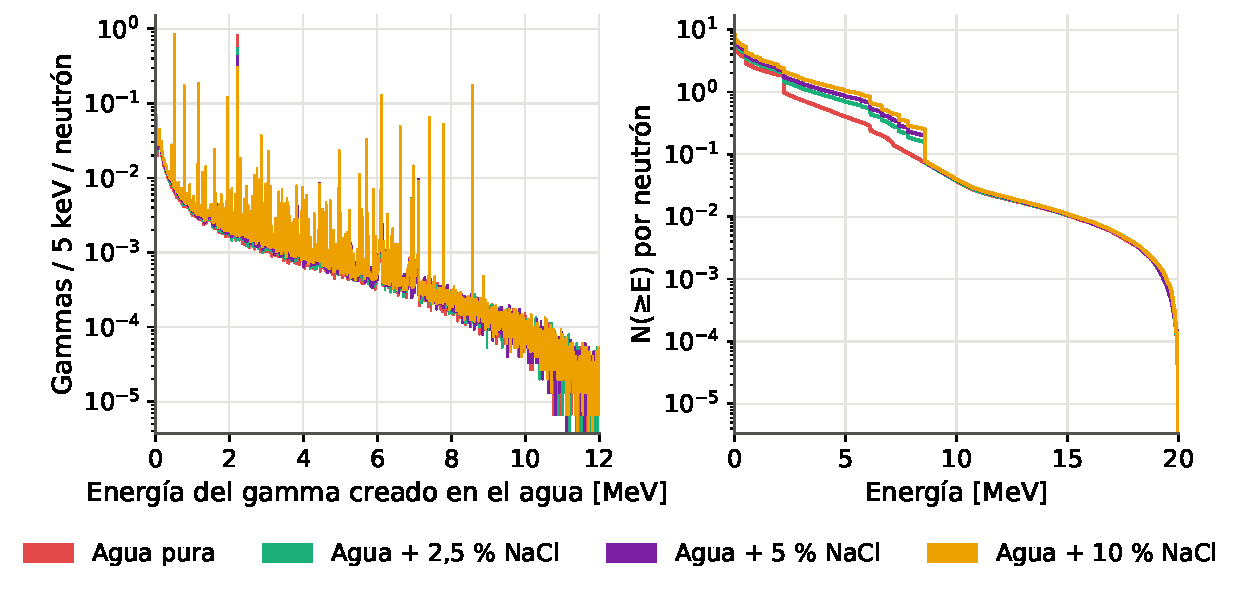
\includegraphics[width=\linewidth]{fig02_espectro_gamma.pdf}
			\vspace{0.2cm}
			\captionsetup{width=\textwidth,justification=justified,singlelinecheck=false}
			\caption[Espectro gamma completo y cuentas acumuladas para neutrones de 500~MeV]{Espectro de energía de los gammas creados en el agua (izquierda, formato de la Fig.~3 de \protect\citet{Sidelnik2020}) y cuentas acumuladas de derecha a izquierda $N(\geq E)$ (derecha, formato de su Fig.~4) para \textcolor{red}{agua pura}, \textcolor{green}{agua + 2.5\,\% de NaCl}, \textcolor{violet}{agua + 5\,\% de NaCl} y \textcolor{orange}{agua + 10\,\% de NaCl}.}
			\label{gama-esp}
		\end{minipage}
	\end{adjustwidth}
\end{figure}

\paragraph{Exceso de cuentas acumuladas entre 2.2 y 8.6~MeV:} En la Figura~(\ref{gama-esp}, derecha) las curvas con NaCl presentan una protuberancia entre 2.2 y 8.6~MeV respecto al agua pura. $N(\geq E)$ cuenta, por neutrón, los gammas de energía mayor o igual que $E$: cada línea produce un escalón en su energía y los gammas comprendidos entre dos energías forman la meseta que las separa. En agua pura casi todos los gammas de captura proceden del H y tienen 2.22~MeV, de modo que por encima de ese escalón no queda ninguno. Con NaCl, el $^{35}$Cl emite su cascada entre 2.3 y 8.58~MeV: esos gammas forman una meseta adicional que termina en un escalón abrupto en 8.58~MeV, la energía de separación del neutrón en $^{36}$Cl, por encima de la cual no puede haber gammas de captura. La Tabla~(\ref{tab:protuberancia}) muestra que la captura explica el 96\,\% (\textcolor{green}{2.5\,\%}), el 94\,\% (\textcolor{violet}{5\,\%}) y el 93\,\% (\textcolor{orange}{10\,\%}) del exceso a 4~MeV, mientras que los gammas de las inelásticas apenas cambian con la sal. El escalón mayor, en 8.58~MeV, corresponde al 27\,\% de las capturas en $^{35}$Cl y es consecuencia del gamma único de $S_n$; con cascadas realistas sería mucho menor y la meseta contendría más gammas de menor energía. Por encima de 8.7~MeV las curvas coinciden, porque solo quedan gammas de las inelásticas, del bremsstrahlung y de las desintegraciones de $\pi^{0}$ y muones, que no dependen de la sal.

\begin{table}[!htbp]
	\centering
	\small
	\captionsetup{width=\linewidth,justification=justified,singlelinecheck=false}
	\caption[Descomposición de las cuentas acumuladas de gammas por proceso]{Descomposición de las cuentas acumuladas $N(\geq E)$ de la Figura~\ref{gama-esp} (derecha) por proceso creador. Gammas creados en el agua por neutrón incidente.}
	\label{tab:protuberancia}
	\renewcommand{\arraystretch}{1.15}
	\resizebox{\textwidth}{!}{\begin{tabular}{lcccc}
		\toprule
		 & \textcolor{red}{\textbf{Agua pura}} & \textcolor{green}{\textbf{2.5\,\% NaCl}} & \textcolor{violet}{\textbf{5\,\% NaCl}} & \textcolor{orange}{\textbf{10\,\% NaCl}} \\
		\midrule
		$N(\geq 4~\mathrm{MeV})$ total & 0.694 & 1.041 & 1.222 & 1.450 \\
		\quad de captura & 0.000 & 0.332 & 0.498 & 0.705 \\
		\quad de inelásticas de neutrones & 0.418 & 0.428 & 0.437 & 0.458 \\
		Exceso sobre el agua pura en $N(\geq 4~\mathrm{MeV})$ & -- & 0.346 & 0.528 & 0.756 \\
		\quad fracción del exceso debida a la captura & -- & 96\,\% & 94\,\% & 93\,\% \\
		Gammas de captura entre 2.3 y 8.7~MeV & 0.000 & 0.463 & 0.694 & 0.984 \\
		\quad por captura en $^{35}$Cl & -- & 1.50 & 1.49 & 1.50 \\
		Escalón de 8.58~MeV (gamma único) & 0.000 & 0.083 & 0.126 & 0.176 \\
		\quad fracción de las capturas en $^{35}$Cl & -- & 27\,\% & 27\,\% & 27\,\% \\
		$N(\geq 8.7~\mathrm{MeV})$ total & 0.216 & 0.216 & 0.219 & 0.217 \\
		\bottomrule
	\end{tabular}}
\end{table}

\begin{figure}[!htbp]
	\begin{adjustwidth}{0cm}{0cm}
		\centering
		\begin{minipage}{\linewidth}
			\centering
			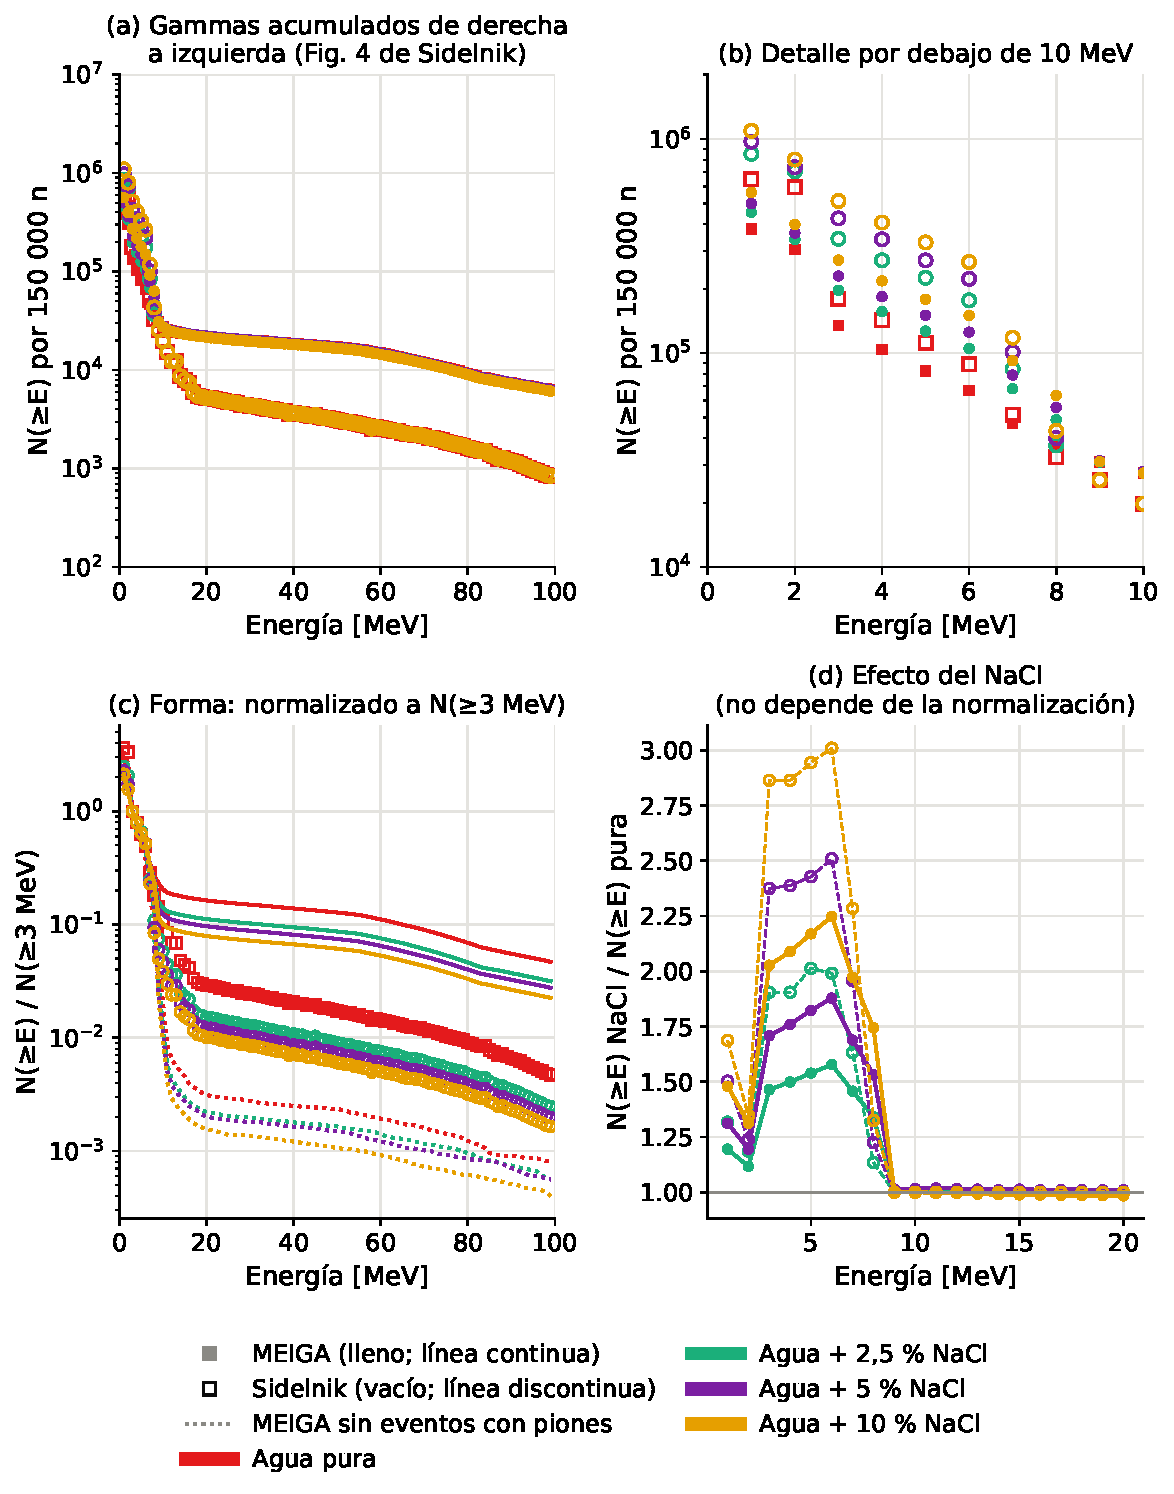
\includegraphics[width=\linewidth]{fig17_gammas_acumulados.pdf}
			\vspace{0.2cm}
			\captionsetup{width=\textwidth,justification=justified,singlelinecheck=false}
			\caption[Gammas acumulados frente a la Fig.~4 de Sidelnik et al.]{Gammas creados en el medio acumulados de derecha a izquierda, en el formato de la Fig.~4 de \protect\citet{Sidelnik2020}: (a) hasta 100~MeV y (b) por debajo de 10~MeV, este trabajo (símbolos llenos) y artículo (símbolos vacíos), cuentas por $1.5\times10^{5}$ neutrones; (c) forma normalizada a $N(\geq3~\mathrm{MeV})$, con y sin los eventos con piones; (d) cociente NaCl / agua pura.}
			\label{fig:gammas-acumulados}
		\end{minipage}
	\end{adjustwidth}
\end{figure}

%==========================================================
\section{Comparación de los espectros de electrones y positrones secundarios}
\label{subsubsec:electrones}
%==========================================================

Los fotones gamma transfieren su energía a electrones y positrones del medio por efecto Compton, efecto fotoeléctrico y producción de pares; solo los que superan el umbral Cherenkov (0.264~MeV de energía cinética en agua) emiten luz. La Figura~(\ref{fig:comparacion-espectros-e}) compara el espectro de los electrones producidos por gammas con la Fig.~5 de \citet[Sec.~3, Fig.~5, p.~2221]{Sidelnik2020}.

\begin{figure}[!htbp]
	\centering
	\includegraphics[width=\linewidth]{espectro-e-ivan.png}\par
	\vspace{0.15cm}
	{\normalsize\bfseries (a) Trabajo previo}\par
	{\small Sidelnik \textit{et al.} (2020)}\par
	\vspace{0.2cm}
	\captionsetup{width=\linewidth,justification=justified,singlelinecheck=false}
	\caption[Comparación de los espectros de electrones producidos por gammas]{Espectros de energía de los electrones producidos por gammas en el agua. (a) Fig.~5 de \protect\citet{Sidelnik2020}. (b) Presente trabajo: espectro con el mismo formato (bines de 20~keV, $1.5\times10^{5}$ neutrones), comparación con la curva digitalizada y los bordes Compton, cociente NaCl / agua pura y saltos en los bordes Compton.}
	\label{fig:comparacion-espectros-e}
\end{figure}

\begin{figure}[!htbp]
	\ContinuedFloat
	\centering
	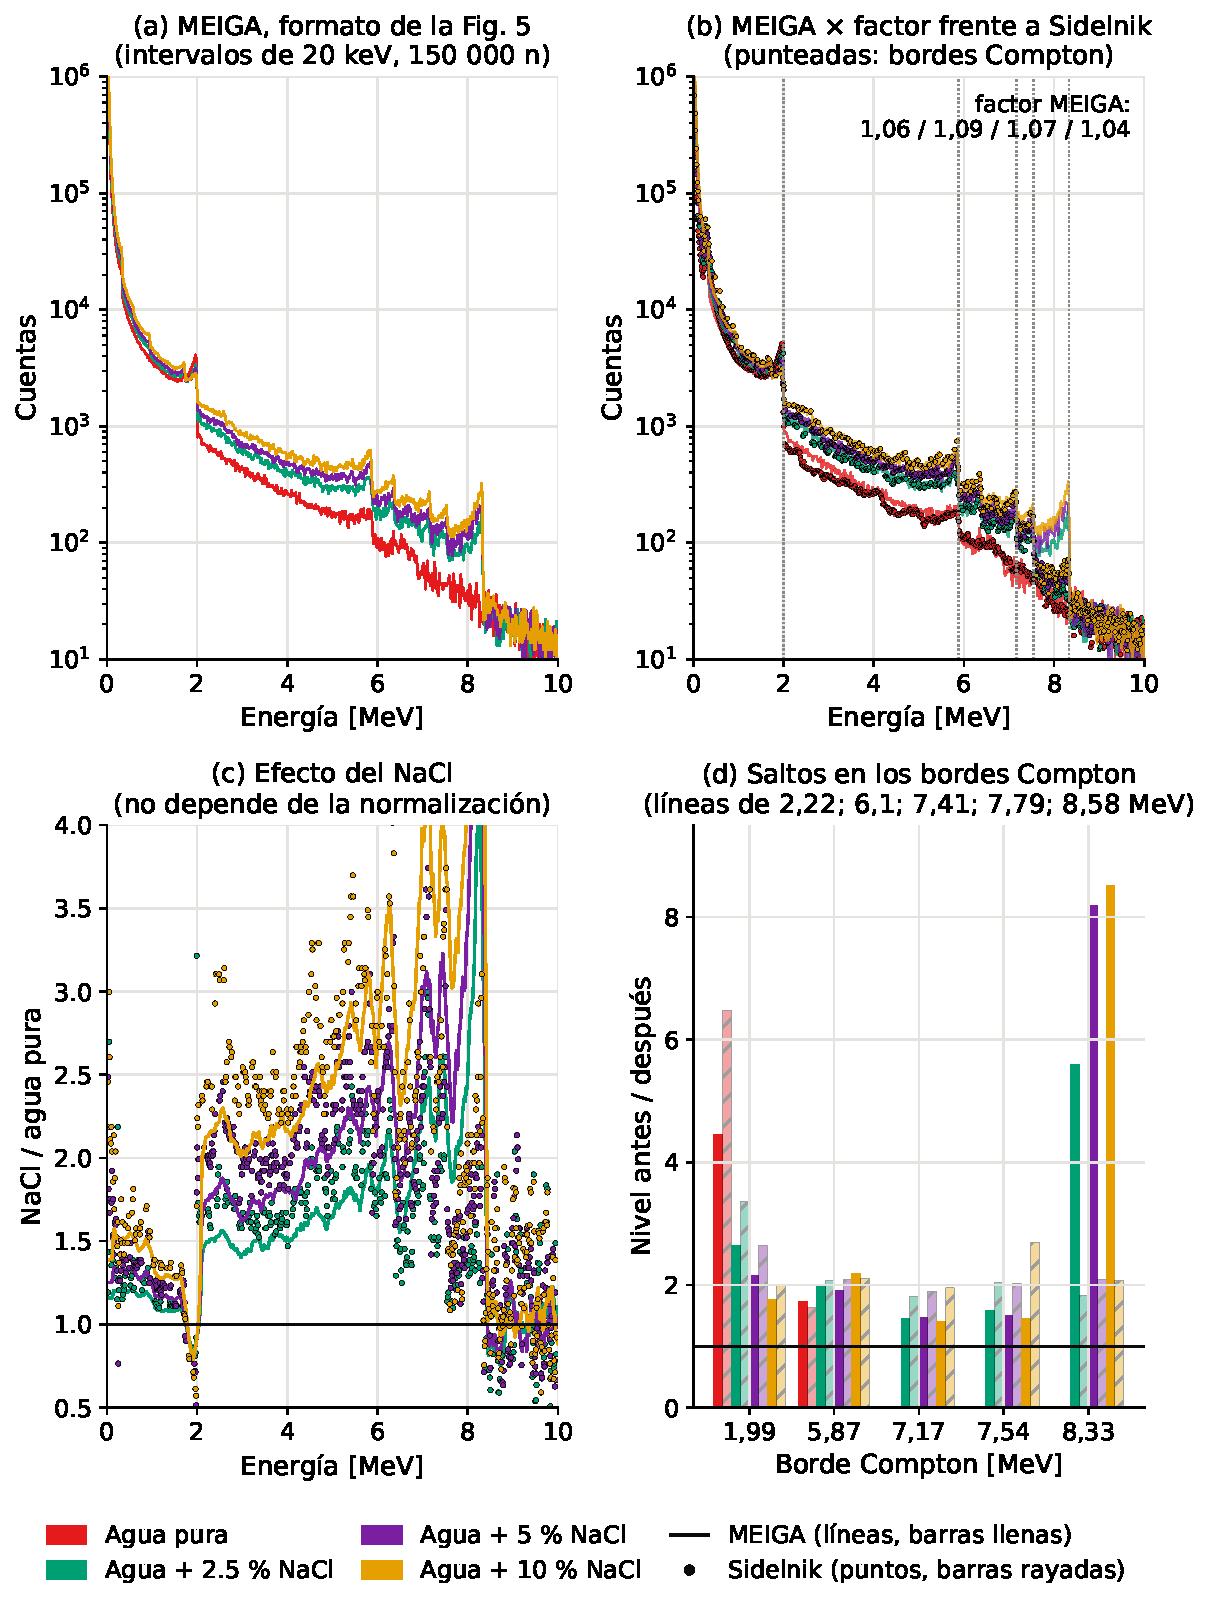
\includegraphics[width=\linewidth]{fig13_espectro_electrones_tipo_sidelnik.pdf}\par
	\vspace{0.15cm}
	{\normalsize\bfseries (b) Presente trabajo}\par
	{\small Reproducción realizada en esta investigación}\par
	\vspace{0.2cm}
	\captionsetup{width=\linewidth,justification=justified,singlelinecheck=false}
	\caption[]{(Continuación) (b) Presente trabajo; véase la descripción en la parte (a) de esta figura.}
\end{figure}

\paragraph{Escala absoluta:} A diferencia de los espectros gamma y de fotones, aquí la comparación no requiere ninguna normalización: ambas figuras representan electrones por $1.5\times10^{5}$ neutrones con intervalos de 20~keV. El factor $k$ del panel (b) de la Figura~\ref{fig:comparacion-espectros-e} es la mediana del cociente Sidelnik/presente trabajo en 11 energías entre 0.5 y 7~MeV: $k=1.06$ (\textcolor{red}{agua pura}), 1.09 (\textcolor{green}{2.5\,\%}), 1.07 (\textcolor{violet}{5\,\%}) y 1.04 (\textcolor{orange}{10\,\%}). Es decir, la presente simulación produce entre un 4 y un 8\,\% menos de electrones que la del artículo, con la misma forma desde 0.3 hasta 10~MeV. Este es el resultado de validación más directo de la cadena gamma $\to$ electrón. El factor es exclusivo de los electrones: el factor 3.40 del espectro gamma (Figura~\ref{fig:comparacion-espectros-gamma-1}) es una normalización, porque el eje de la Fig.~3 del artículo está en unidades arbitrarias.

\paragraph{Origen de la diferencia de amplitud:} Se identifican cuatro causas.
\begin{enumerate}[label=(\roman*)]
	\item \textbf{Probabilidad de captura.} Es la causa principal: el cociente entre las probabilidades de captura del artículo y de la presente simulación (Tabla~\ref{tab:defs-captura}) es 1.05, 1.09, 1.10 y 1.12 para los cuatro medios, prácticamente igual a $k$ en \textcolor{red}{agua pura} y con \textcolor{green}{2.5\,\%} de NaCl. Con 5 y 10\,\% el factor $k$ queda por debajo de ese cociente porque cada captura en $^{35}$Cl emite en la simulación más energía que la real (10.1 frente a 8.58~MeV; Sec.~\ref{subsubsec:nucleos-captura-neutrones}) y genera más electrones, lo que compensa en parte las capturas faltantes; el efecto crece con la concentración.
	\item \textbf{Diferencias de forma.} El factor $k$ es un promedio: punto a punto el cociente varía entre 0.85 y 1.35 en \textcolor{red}{agua pura}. El artículo está por encima justo debajo del borde Compton de 1.994~MeV y la simulación entre 2 y 3~MeV, donde domina el fondo de desexcitación nuclear; con NaCl, entre 7.4 y 8.3~MeV la simulación queda muy por encima por el gamma único de 8.58~MeV.
	\item \textbf{Digitalización.} La Fig.~5 del artículo se digitalizó por color en escala logarítmica, con una incertidumbre del 5--10\,\% en las cuentas.
	\item \textbf{Modelos de simulación.} Las versiones de \textsc{Geant4} y las listas físicas son distintas, y el artículo no las especifica.
\end{enumerate}
\noindent La diferencia de amplitud es, por tanto, pequeña y se explica casi por completo por la probabilidad de captura; las diferencias físicamente relevantes están en la forma del espectro (fondo de desexcitación nuclear y gamma único de 8.58~MeV), que se analizan a continuación.

\paragraph{Bordes Compton:} En ambas simulaciones se identifican los bordes Compton de la línea de aniquilación (0.34~MeV), de la captura en H (1.994~MeV) y de la línea de 6.13/6.11~MeV (5.87~MeV), cuya energía es
\begin{equation}
	T_{\max} = \frac{2E_{\gamma}^{2}}{m_{e}c^{2}+2E_{\gamma}} .
\end{equation}
El salto en el borde de 1.994~MeV es 4.5 en este trabajo y 6.5 en el artículo; el de 5.87~MeV, 1.74 y 1.63.

\paragraph{Interpretación de las diferencias:} Para entender las diferencias se clasificó cada electrón según el origen del gamma que lo produce (Figura~\ref{fig:origen-electrones}). Por debajo del borde de 1.994~MeV el 76\,\% de los electrones procede de la línea de 2.223~MeV; por encima, el 78\,\% procede de gammas de la dispersión inelástica de neutrones en el oxígeno (desexcitación de $^{16}$O$^{*}$, $^{12}$C$^{*}$ y $^{15}$N$^{*}$). El salto vale por tanto $J\approx1+C_{\mathrm{H}}/F$, donde $C_{\mathrm{H}}$ son los electrones de la captura en H y $F$ ese fondo. Para obtener el salto del artículo habría que dividir el fondo de la simulación por 1.60 en \textcolor{red}{agua pura} y por 1.76 con \textcolor{green}{2.5\,\% de NaCl}, un factor similar en ambos medios, como corresponde a un fondo que no depende de la sal. Es decir, por cada captura en H la presente simulación produce $\approx$\,1.6 veces más gammas de desexcitación nuclear, en acuerdo con el espectro gamma acumulado. Los piones no son la causa (sin ellos el salto pasa de 4.46 a 4.58); la diferencia depende del modelo de cascada y de la desexcitación de los núcleos residuales, que cambiaron entre versiones de \textsc{Geant4}.

\paragraph{Efecto del NaCl:} El cociente NaCl / agua pura no depende de la normalización. Por debajo del borde de 1.994~MeV vale $\approx$\,0.84 en las dos simulaciones, porque el Cl compite con el H y las capturas en H por neutrón caen de 0.83 a 0.55; que el valor coincida indica que la competencia H/Cl es la misma en ambas. Entre 2 y 6~MeV, donde contribuyen los electrones Compton de las líneas del Cl, el cociente vale 1.42--1.96 en este trabajo y 1.63--2.19 en el artículo: el fondo más alto diluye la contribución del Cl. Entre 7 y 8.3~MeV el cociente simulado (2.46) supera al del artículo (1.58) por los electrones Compton del gamma único de 8.58~MeV. Las intensidades de las líneas intermedias del Cl coinciden con el artículo porque las dos limitaciones de \textsc{Geant4} se compensan: hay $\approx$\,1.27 veces más capturas en Cl, pero solo el $\approx$\,76\,\% sigue una cascada ($1.27\times0.76\approx0.97$).

\begin{figure}[!htbp]
	\begin{adjustwidth}{0cm}{0cm}
		\centering
		\begin{minipage}{\linewidth}
			\centering
			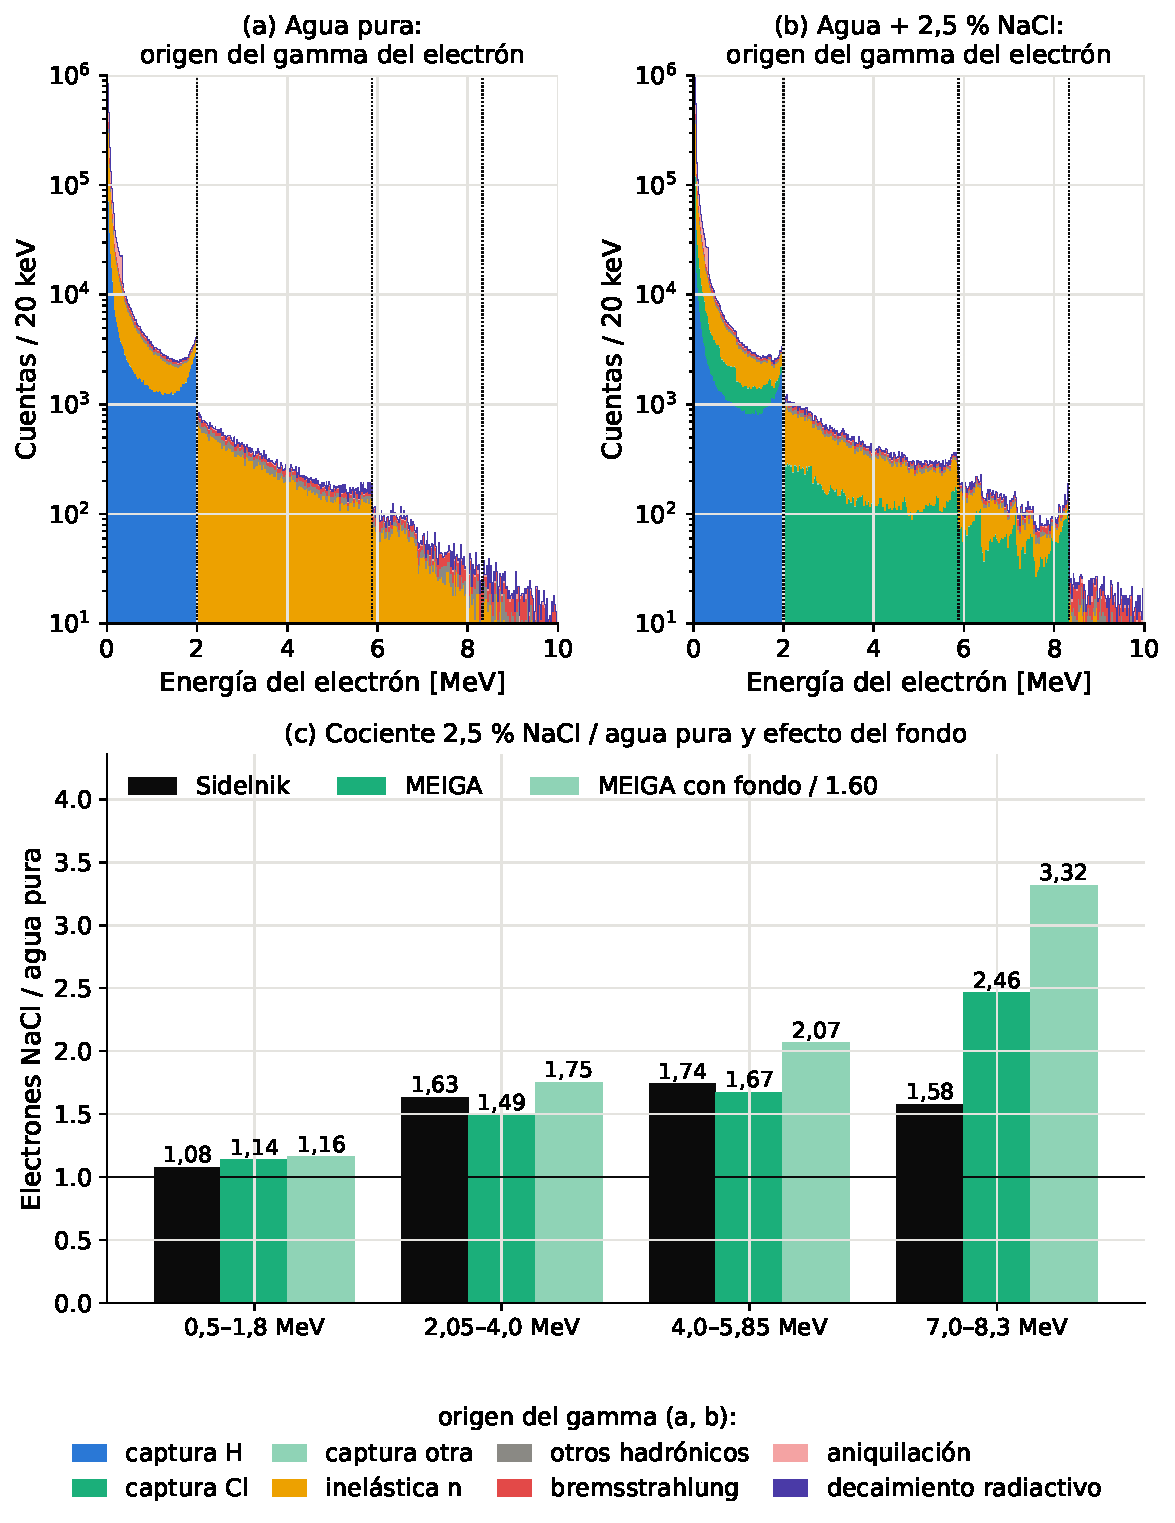
\includegraphics[width=\linewidth,height=0.78\textheight,keepaspectratio]{fig14_origen_electrones.pdf}
			\vspace{0.2cm}
			\captionsetup{width=\textwidth,justification=justified,singlelinecheck=false}
			\caption[Origen de los electrones producidos por gammas]{Origen del gamma que produce cada electrón en \textcolor{red}{agua pura} y \textcolor{green}{agua + 2.5\,\% de NaCl} (áreas apiladas), y cociente NaCl / agua pura en cuatro intervalos de energía: \protect\citet{Sidelnik2020}, este trabajo y este trabajo con el fondo no debido a capturas dividido por el factor que reproduce el salto en el borde de 1.994~MeV del artículo.}
			\label{fig:origen-electrones}
		\end{minipage}
	\end{adjustwidth}
\end{figure}

%==========================================================
\section{Distribución de energía de los deuterones producidos en la captura de neutrones sobre hidrógeno}
\label{subsubsec:deuterones}
%==========================================================

En la captura $n+p\to d+\gamma$ el deuterón retrocede con una energía
\begin{equation}
	E_{d} \simeq \frac{E_{\gamma}^{2}}{2M_{d}c^{2}} = \frac{(2.2244~\mathrm{MeV})^{2}}{2\times1875.6~\mathrm{MeV}} = 1.319~\mathrm{keV}.
\end{equation}
La distribución simulada (Figura~\ref{masa-deu}) tiene su máximo exactamente en ese valor (mediana 1.319~keV) y una anchura $\sigma=9.9$~eV, originada en el movimiento térmico del neutrón y del protón en el instante de la captura, la misma causa que da a la línea de 2.224~MeV su anchura. Con NaCl el pico desciende en proporción a la fracción de capturas en H (64, 48 y 31\,\% con \textcolor{green}{2.5}, \textcolor{violet}{5} y \textcolor{orange}{10\,\%} de NaCl); su posición no cambia (1.319~keV) y su anchura crece (10.5, 10.8 y 11.6~eV). La media y el valor cuadrático medio de la distribución no describen el pico: los dominan unos pocos deuterones (0.12\,\%) procedentes de capturas de neutrones aún rápidos, con energías de hasta 6.9~MeV (media 1.43~keV y RMS 23.2~keV en \textcolor{red}{agua pura}). 
%Por ello se recomienda caracterizar el pico con la mediana y la $\sigma$ en la ventana de 1.20--1.45~keV.

\begin{figure}[!htbp]
	\begin{adjustwidth}{0cm}{0cm}
		\centering
		\begin{minipage}{\linewidth}
			\centering
			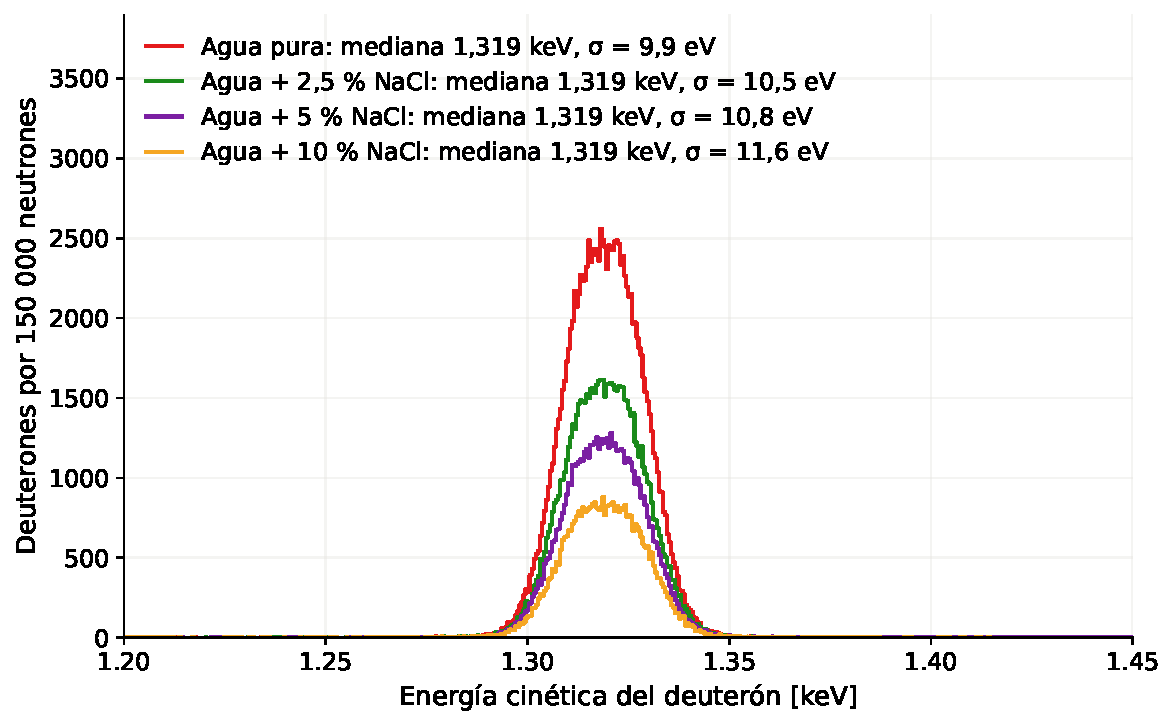
\includegraphics[width=\linewidth]{fig16_deuterones_captura.pdf}
			\vspace{0.2cm}
			\captionsetup{width=\textwidth,justification=justified,singlelinecheck=false}
			\caption[Energía de los deuterones producidos en la captura de neutrones en hidrógeno]{Energía cinética de los deuterones producidos en la captura $^{1}\mathrm{H}(n,\gamma)^{2}\mathrm{H}$ para los cuatro medios; cuentas por $1.5\times10^{5}$ neutrones primarios.}
			\label{masa-deu}
		\end{minipage}
	\end{adjustwidth}
\end{figure}

%==========================================================
\section{Comparación de la distribución de fotones Cherenkov detectados para neutrones de 500~MeV}
\label{subsubsec:cherenkov}
%==========================================================

\citet[Sec.~3, Fig.~6, p.~2221]{Sidelnik2020} presentan la distribución del número de fotones Cherenkov aceptados por la eficiencia cuántica del PMT. Para comparar con esa figura se utilizó el mismo observable: para cada neutrón se cuentan los fotones Cherenkov aceptados por la eficiencia cuántica del R5912 en el momento de crearse, antes del transporte óptico (en el modo \texttt{eFast} del simulador son exactamente los fotones que se transportan); se descartan los eventos sin ningún fotón aceptado (39\,\% de los neutrones), porque la figura de referencia no muestra el pico en cero; y se histograma con bines de 10 fotones entre 0 y 2500 fotones, en escala logarítmica y en cuentas absolutas, sin normalizar ni reescalar. La Figura~(\ref{fig:comparacion-carga}) muestra el resultado.

\begin{figure}[!htbp]
	\begin{adjustwidth}{0cm}{0cm}
		\centering
		\begin{minipage}{\linewidth}
			\centering
			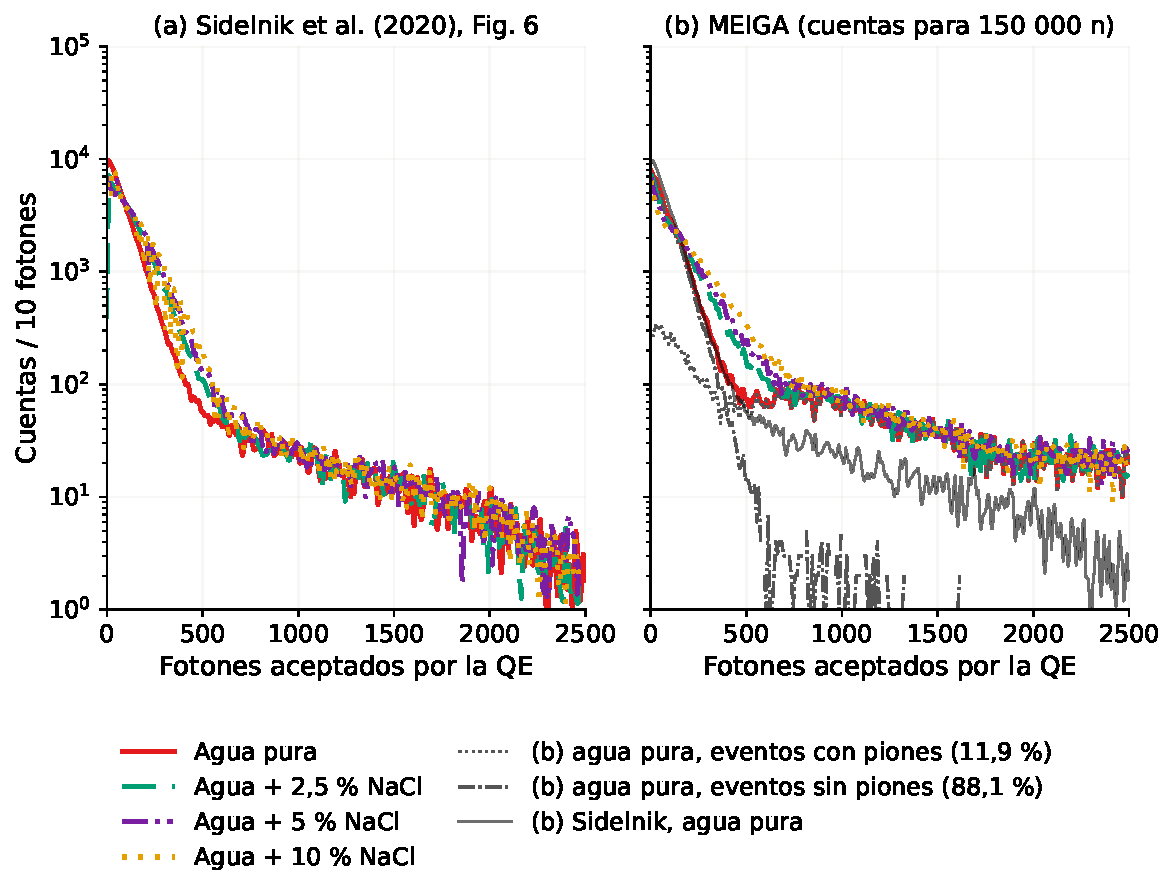
\includegraphics[width=\linewidth]{fig10_figura6_sidelnik_vs_meiga.pdf}
			\vspace{0.2cm}
			\captionsetup{width=\textwidth,justification=justified,singlelinecheck=false}
			\caption[Comparación de la distribución de fotones Cherenkov aceptados]{Distribución del número de fotones Cherenkov aceptados por la eficiencia cuántica del PMT para neutrones de 500~MeV. Izquierda: Fig.~6 de \protect\citet{Sidelnik2020}, digitalizada. Derecha: la misma figura construida con el presente modelo ($1.5\times10^{5}$ neutrones por medio) para los cuatro medios, con la curva del artículo superpuesta y los eventos de agua pura separados según haya o no producción de piones.}
			\label{fig:comparacion-carga}
		\end{minipage}
	\end{adjustwidth}
\end{figure}

\paragraph{Coincidencia hasta 500 fotones:} Entre 0 y 500 fotones la distribución simulada coincide con la del trabajo de referencia sin ningún reescalamiento: la pendiente es la misma, el quiebre aparece en 400--500 fotones y las cuentas absolutas coinciden dentro del 6--23\,\% (Tabla~\ref{tab:fotones-intervalos}). La correlación de la forma en escala logarítmica entre 0 y 1000 fotones es 0.985. El número de neutrones, la eficiencia cuántica y la producción de luz Cherenkov son, por tanto, comparables en las dos simulaciones.

\begin{table}[!htbp]
	\centering
	\small
	\captionsetup{width=\linewidth,justification=justified,singlelinecheck=false}
	\caption[Cuentas por intervalo de fotones aceptados y producción de piones]{Cuentas absolutas por intervalo de fotones aceptados en \textcolor{red}{agua pura} (eventos con al menos un fotón) y fracción de eventos con producción de piones en alguna interacción inelástica de un neutrón. Un mismo evento puede tener piones cargados y neutros.}
	\label{tab:fotones-intervalos}
	\renewcommand{\arraystretch}{1.15}
	\resizebox{\textwidth}{!}{
	\begin{tabular}{lrrcccc}
		\toprule
		\textbf{Fotones aceptados} & \textbf{Este trabajo} & \textbf{\makecell{Sidelnik et al.\\(digitalizada)}} & \textbf{Razón} & \textbf{Con $\pi^{\pm}$} & \textbf{Con $\pi^{0}$} & \textbf{Con algún pion} \\
		\midrule
		1 -- 100 & 52\,395 & 67\,941 & 0.77 & 4.0\,\% & 1.5\,\% & 5.5\,\% \\
		100 -- 500 & 28\,902 & 30\,773 & 0.94 & 13.5\,\% & 2.6\,\% & 16.1\,\% \\
		500 -- 1000 & 3\,748 & 1\,758 & 2.13 & 68.6\,\% & 26.5\,\% & 95.1\,\% \\
		1000 -- 2500 & 4\,783 & 1\,495 & 3.20 & 35.5\,\% & 63.1\,\% & 98.6\,\% \\
		$\geq$ 2500 & 1\,707 & -- & -- & 9.7\,\% & 89.3\,\% & 98.8\,\% \\
		\bottomrule
	\end{tabular}}
\end{table}

\paragraph{La cola por encima de 500 fotones: producción de piones:} Por encima de 500 fotones la simulación presenta entre dos y tres veces más eventos que el trabajo de referencia. Solo el 11.9\,\% de los neutrones produce piones, pero esos eventos forman la cola: el 97.3\,\% de los eventos con 500 fotones o más contiene piones. Un evento con piones produce en promedio 944 fotones aceptados, frente a 49 en uno sin piones. Los $\pi^{\pm}$ emiten luz Cherenkov a lo largo de su trayectoria y, al desintegrarse, producen muones que también la emiten; los $\pi^{0}$ se desintegran en dos gammas de $\approx$\,70~MeV que inician cascadas electromagnéticas. Sin los eventos con piones, la distribución cae a cero hacia 600 fotones. La energía de 500~MeV está apenas por encima del umbral de producción de piones en colisiones nucleón--nucleón ($\approx$\,290~MeV), donde la sección eficaz depende fuertemente del modelo hadrónico; la explicación más probable es que la simulación de referencia usara otra lista física u otra versión de \textsc{Geant4}, que el artículo no especifica. La cola no afecta al intervalo de 0 a 500 fotones, que corresponde a la moderación y la captura.

\paragraph{Efecto del NaCl en la luz Cherenkov:} Con el mismo observable, el presente modelo reproduce el efecto del NaCl de la Fig.~6 del artículo: las curvas con NaCl quedan por encima de la de agua pura, más cuanto mayor es la concentración, entre $\approx$\,150 y 550 fotones, por la luz adicional de las capturas en Cl; por encima de 600 fotones las curvas coinciden (piones). Entre 100 y 500 fotones las cuentas aumentan un 30.1\,\% (\textcolor{green}{2.5\,\%}), un 42.8\,\% (\textcolor{violet}{5\,\%}) y un 59.2\,\% (\textcolor{orange}{10\,\%}) en este trabajo, frente al 52.9\,\%, 66.9\,\% y 53.9\,\% del artículo, y la correlación de forma con la curva correspondiente de Sidelnik et al. es 0.989, 0.994 y 0.982. En la presente simulación el aumento es monótono con la concentración; en la figura digitalizada del artículo, en cambio, la curva de 10\,\% no supera a la de 5\,\% en este intervalo. Los fotones Cherenkov creados por neutrón pasan de 1\,441 (\textcolor{red}{agua pura}) a 1\,662 (\textcolor{green}{2.5\,\%}), 1\,806 (\textcolor{violet}{5\,\%}) y 1\,994 (\textcolor{orange}{10\,\%}).

\paragraph{Contribución de los piones al déficit del efecto del NaCl:} Para cuantificar qué parte de la diferencia con el artículo se debe a la mayor producción de piones, se marcó cada neutrón cuyo árbol de interacciones contiene una inelástica con producción de $\pi^{\pm}$ o $\pi^{0}$. Estos eventos son el 11.9--12.1\,\% en los cuatro medios. Al excluirlos, el aumento de cuentas entre 100 y 500 fotones pasa de 30.1 a 33.5\,\% (\textcolor{green}{2.5\,\%}), de 42.8 a 48.8\,\% (\textcolor{violet}{5\,\%}) y de 59.2 a 68.7\,\% (\textcolor{orange}{10\,\%}), frente a 52.9, 66.9 y 53.9\,\% en el artículo (Figura~\ref{fig:piones-nacl}). Los piones explican, por tanto, solo unos 3 y 6 de los 23 y 24 puntos de diferencia con 2.5 y 5\,\% de NaCl: el exceso de cuentas que aporta la sal casi no cambia al excluirlos, y lo que se modifica es el fondo del agua pura con el que se compara. El resto del déficit se atribuye al fondo de desexcitación nuclear tras las interacciones inelásticas, $\approx$\,1.6 veces mayor por captura en H en la presente simulación (Sec.~\ref{subsubsec:electrones}), y al menor aumento de la probabilidad de captura con la sal (Sec.~\ref{subsubsec:captura}). Ambos dependen del modelo hadrónico y de los datos de captura empleados, y su verificación requiere corridas adicionales con otras listas físicas. Con 10\,\% de NaCl la simulación ya supera al artículo, y la diferencia crece al excluir los piones, lo que es consistente con la anomalía de la curva de 10\,\% del artículo, que apenas supera a la de 5\,\%.

\begin{figure}[!htbp]
	\centering
	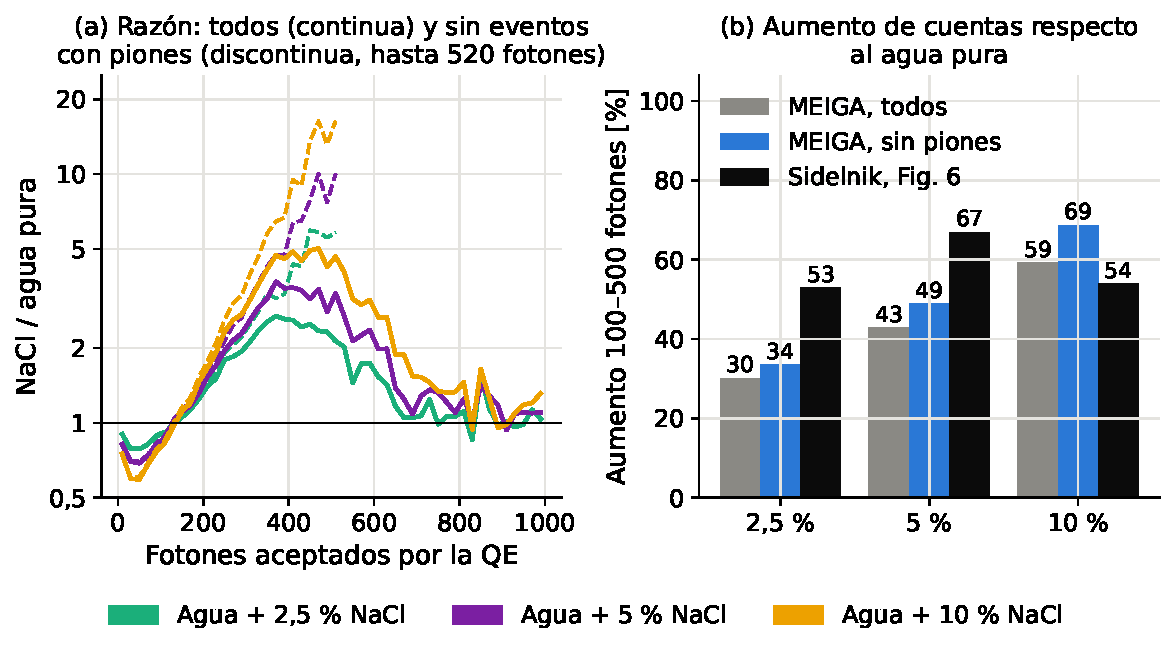
\includegraphics[width=\linewidth]{fig24_piones_efecto_nacl.pdf}
	\vspace{0.2cm}
	\captionsetup{width=\textwidth,justification=justified,singlelinecheck=false}
	\caption[Efecto del NaCl en la distribución de fotones con y sin piones]{Efecto del NaCl en la distribución de fotones Cherenkov aceptados, con y sin los eventos con producción de piones. (a) Razón NaCl/agua pura para todos los eventos (línea continua) y sin los eventos con piones (línea discontinua, hasta 520 fotones). (b) Aumento de cuentas entre 100 y 500 fotones respecto al \textcolor{red}{agua pura}: presente trabajo con todos los eventos y sin los eventos con piones, frente a la Fig.~6 de \protect\citet{Sidelnik2020}.}
	\label{fig:piones-nacl}
\end{figure}

%==========================================================
\section{Validación cuantitativa de los histogramas de carga}
\label{subsubsec:validacion-cuantitativa}
%==========================================================

Con el propósito de cuantificar la concordancia del efecto del NaCl, se calculó la razón entre el histograma de fotones aceptados de cada solución salina y el del agua pura, tanto para la presente simulación como para las curvas digitalizadas de la Fig.~6 de \citet{Sidelnik2020}. Como ambos conjuntos corresponden al mismo número de neutrones ($1.5\times10^{5}$ por medio), la razón se calcula con cuentas absolutas, sin normalizar por el área. Para reducir las fluctuaciones de Poisson los histogramas se agruparon en bines de 50 fotones, y se excluyó el primer bin (0--50 fotones), afectado por la digitalización. La Figura~(\ref{fig:ratio_comparison}) muestra las curvas de razón.

\begin{figure}[!htbp]
	\begin{adjustwidth}{0cm}{0cm}
		\centering
		\begin{minipage}{\linewidth}
			\centering
			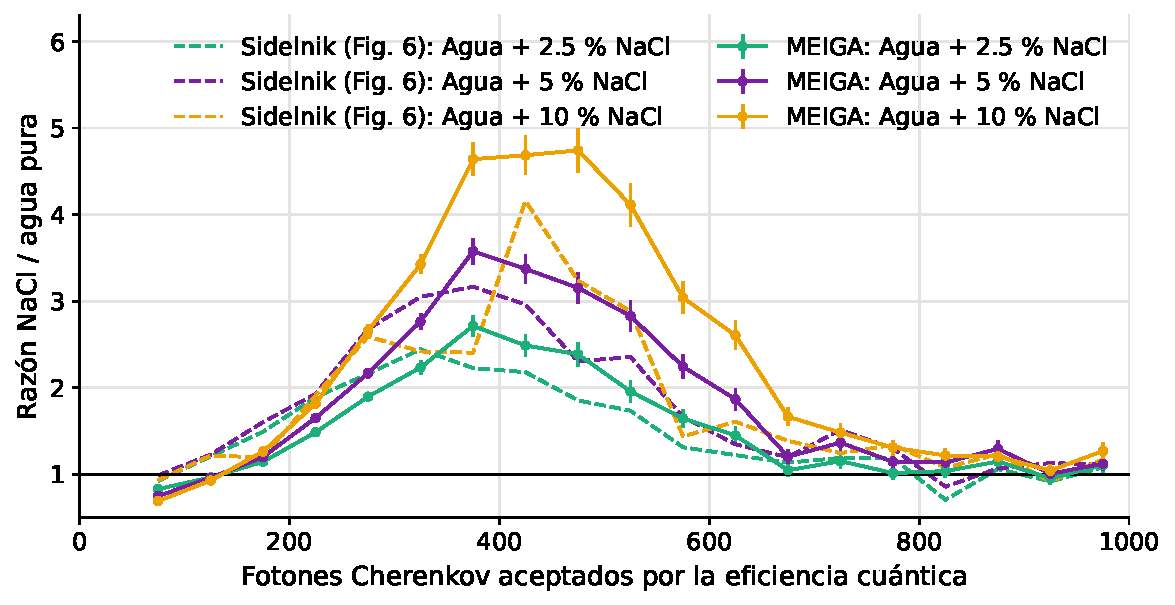
\includegraphics[width=\linewidth]{fig22_razon_histogramas.pdf}
			\vspace{0.2cm}
			\captionsetup{width=\textwidth,justification=justified,singlelinecheck=false}
			\caption[Razón de los histogramas de fotones aceptados entre NaCl y agua pura]{Razón entre los histogramas de fotones Cherenkov aceptados por la eficiencia cuántica de cada solución salina y del agua pura, en bines de 50 fotones: presente trabajo (puntos con barras de error estadístico) y Fig.~6 de \protect\citet{Sidelnik2020} digitalizada (líneas discontinuas), para \textcolor{green}{agua + 2.5\,\% de NaCl}, \textcolor{violet}{agua + 5\,\% de NaCl} y \textcolor{orange}{agua + 10\,\% de NaCl}.}
			\label{fig:ratio_comparison}
		\end{minipage}
	\end{adjustwidth}
\end{figure}

Las curvas de los dos trabajos presentan las mismas características:
\begin{itemize}
	\item Para un número reducido de fotones ($N<150$) la razón permanece por debajo de la unidad: la captura en Cl desplaza eventos desde la región de baja señal hacia valores mayores.
	\item Entre 150 y 400 fotones la razón crece para todas las concentraciones, manteniendo el orden \textcolor{orange}{10\,\%} $>$ \textcolor{violet}{5\,\%} $>$ \textcolor{green}{2.5\,\%}, como consecuencia de la luz adicional de las capturas en $^{35}$Cl.
	\item El máximo aparece entre 375 y 475 fotones en este trabajo y entre 325 y 425 fotones en el artículo, con valores de 2.72, 3.58 y 4.74 (este trabajo) frente a 2.44, 3.17 y 4.16 (Sidelnik et al.) para 2.5, 5 y 10\,\% de NaCl. En ambos trabajos el máximo se desplaza hacia más fotones al aumentar la concentración.
	\item Por encima de $\approx$\,700 fotones las razones tienden a la unidad: la cola está dominada por los eventos con piones, que no dependen de la sal.
	\item La razón media entre 100 y 500 fotones coincide dentro del 1\,\% para 2.5 y 5\,\% de NaCl: 1.92 frente a 1.93 (\textcolor{green}{2.5\,\%}) y 2.36 frente a 2.37 (\textcolor{violet}{5\,\%}). Con \textcolor{orange}{10\,\%} es 3.02 en este trabajo y 2.39 en el artículo, donde la curva digitalizada de 10\,\% apenas supera a la de 5\,\% en este intervalo.
\end{itemize}

\paragraph{Análisis cuantitativo de las curvas de razón:} La concordancia se evaluó con métricas de correlación (coeficientes de Pearson $r$ y de Spearman $\rho$) y de error (RMSE y MAE) entre las curvas de razón de los dos trabajos, en los 19 bines entre 50 y 1000 fotones (Tabla~\ref{tab:metricas_validacion}).

\begin{table}[!htbp]
	\centering
	\begin{minipage}{\textwidth}
		\centering
		\captionsetup{type=table,width=\linewidth,margin=0pt,justification=justified,singlelinecheck=false}
		\captionof{table}[Métricas estadísticas de validación entre las curvas de razón simuladas y de referencia.]{Métricas estadísticas de concordancia entre las curvas de razón NaCl / agua pura obtenidas en el presente trabajo y las curvas digitalizadas de la Fig.~6 de \protect\citet{Sidelnik2020}, en 19 bines de 50 fotones entre 50 y 1000 fotones aceptados.}
		\label{tab:metricas_validacion}
		\vspace{0.25cm}
		\renewcommand{\arraystretch}{1.30}
		\setlength{\tabcolsep}{2pt}
		\begin{tabularx}{\linewidth}{
				>{\centering\arraybackslash}p{0.10\linewidth}
				>{\centering\arraybackslash}p{0.08\linewidth}
				>{\centering\arraybackslash}p{0.14\linewidth}
				>{\centering\arraybackslash}p{0.08\linewidth}
				>{\centering\arraybackslash}p{0.10\linewidth}
				>{\centering\arraybackslash}p{0.09\linewidth}
				>{\centering\arraybackslash}p{0.15\linewidth}
				>{\centering\arraybackslash}X}
			\toprule
			\textbf{NaCl} & $\mathbf{r}$ & $\mathbf{p}$ & $\boldsymbol{\rho}$ & \textbf{RMSE} & \textbf{MAE} & \textbf{\makecell{Razón media\\100--500}} & \textbf{Nivel} \\
			\midrule
			\textcolor{green}{2.5\,\%} & 0.881 & $6.2\times10^{-7}$ & 0.863 & 0.276 & 0.234 & 1.92 / 1.93 & Alta \\[1pt]
			\textcolor{violet}{5\,\%} & 0.906 & $9.1\times10^{-8}$ & 0.867 & 0.383 & 0.325 & 2.36 / 2.37 & Alta \\[1pt]
			\textcolor{orange}{10\,\%} & 0.895 & $2.2\times10^{-7}$ & 0.930 & 0.857 & 0.569 & 3.02 / 2.39 & Alta en forma \\
			\bottomrule
		\end{tabularx}
		\vspace{0.1cm}
		\begin{minipage}{0.98\textwidth}
			\footnotesize \textit{Nota:} La razón media se da como este trabajo / Sidelnik et al. Los valores de $p$ corresponden a la hipótesis de correlación nula de Pearson. Las métricas de la versión anterior de esta tabla se calcularon con 700 puntos digitalizados interpolados, lo que producía valores de $p$ artificialmente pequeños; aquí se usan bines independientes.
		\end{minipage}
	\end{minipage}
\end{table}

Las tres concentraciones presentan correlaciones altas ($r=0.88$, $0.91$ y $0.90$; $\rho=0.86$, $0.87$ y $0.93$) con $p<10^{-6}$: la forma de las curvas de razón, incluida la posición del máximo y su desplazamiento con la concentración, se reproduce en todos los casos. Las diferencias de amplitud, cuantificadas por RMSE y MAE, crecen con la concentración y se concentran en la región del máximo, donde la razón simulada es un 11--14\,\% mayor que la del artículo y está desplazada 0--50 fotones hacia valores mayores. Este exceso es coherente con la sobreestimación de la energía de las capturas en Cl descrita en la Sec.~\ref{subsubsec:nucleos-captura-neutrones}, que aumenta la luz por captura en Cl. Con 10\,\% de NaCl, además, la diferencia en la razón media (3.02 frente a 2.39) proviene principalmente de la curva digitalizada del artículo, cuyo efecto entre 100 y 500 fotones es prácticamente igual al de 5\,\%; en la presente simulación el efecto crece de forma monótona con la concentración, como lo hacen la probabilidad de captura, el tiempo de captura y la energía gamma de captura (Tabla~\ref{tab:efecto-nacl-captura}). A diferencia de la comparación anterior, la correlación no disminuye al aumentar la concentración.

\paragraph{Del número de fotones aceptados a la carga en el PMT:} El eje de la Fig.~6 del trabajo de referencia corresponde a los fotones Cherenkov aceptados por la eficiencia cuántica. Su escala y su forma coinciden con los fotones aceptados en el momento de su creación, antes del transporte óptico, y no con la carga en el PMT, que es unas 16 veces menor; esto indica que la figura no incluye la eficiencia de colección óptica, aunque el artículo no lo especifica. La magnitud que mide el detector es, en cambio, la carga en el PMT, que incluye el transporte de cada fotón por el agua y sus reflexiones en el Tyvek hasta alcanzar el fotocátodo. La Tabla~(\ref{tab:balance-luz}) resume el balance de luz en \textcolor{red}{agua pura}: de los 1\,441 fotones Cherenkov creados por neutrón, 155.6 (10.8\,\%) son aceptados por la eficiencia cuántica y 9.81 (6.3\,\% de los transportados) alcanzan el PMT. La pérdida dominante es la absorción en la pared, y puede describirse con un modelo de rebotes ajustado a las trayectorias simuladas. En cada encuentro con la pared el fotón alcanza el PMT con probabilidad $s$; si no, choca con el Tyvek, donde se absorbe con probabilidad $a$; y entre dos encuentros puede absorberse en el agua con probabilidad $w$. La fracción de fotones que llega al PMT es entonces
\begin{equation}
	P_{\mathrm{PMT}} = \frac{s}{s+(1-s)\,a+w}.
	\label{eq:modelo-rebotes}
\end{equation}
\noindent En \textcolor{red}{agua pura} se miden $s=0.8$\,\%, $a=9.8$\,\% y $w=2.0$\,\%, con los que la Ec.~(\ref{eq:modelo-rebotes}) da $P_{\mathrm{PMT}}=6.3$\,\%, igual al valor observado. Un fotón sobrevive en promedio $1/a\approx10$ choques con el Tyvek (7.1 rebotes medios, porque también se pierde en el agua), mientras que para encontrar el PMT por azar necesitaría del orden de $1/s\approx130$ encuentros con la pared (Figura~\ref{fig:destino-fotones}).

La absorción por choque, $a=9.8$\,\%, tiene tres componentes. La reflectividad medida del Tyvek, tabulada en el código de MEIGA según la energía del fotón (0.99--1.00 en el azul y 0.78--0.85 en el ultravioleta), aporta $1-R_{\mathrm{tabla}}\approx2.1$ puntos. En el código, sin embargo, esa tabla se multiplica por un factor de escala \texttt{scaleLinerRef}\,=\,0.94 (\texttt{Materials.cc}), de modo que la reflectividad empleada es $R=0.94\,R_{\mathrm{tabla}}$; este factor añade $\approx5.9$ puntos, porque impone una pérdida mínima del 6\,\% en cada choque aun donde el Tyvek tabulado refleja el 100\,\%. Los $\approx1.9$ puntos restantes son una pérdida adicional del modelo de superficie \texttt{groundbackpainted} de \textsc{Geant4}. El factor 0.94 es, por tanto, el principal responsable de la absorción en la pared. Es un parámetro del modelo sin una justificación documentada; factores de este tipo se emplean a veces para representar un revestimiento envejecido o contaminado.

La Tabla~(\ref{tab:sensibilidad-tyvek}) estima, con la Ec.~(\ref{eq:modelo-rebotes}) aplicada por intervalos de energía del fotón, la carga media que se obtendría con otros modelos ópticos. La escala absoluta de la carga es incierta en un factor de hasta $\approx2.5$. Esta incertidumbre no afecta a la comparación con la Fig.~6 del artículo, que usa los fotones aceptados antes del transporte, ni a las diferencias entre medios, porque el transporte óptico es el mismo en los cuatro. En esta campaña se conservó el modelo del Tyvek para mantener la comparabilidad entre todas las corridas; su revisión queda como trabajo futuro.

La distribución de fotones aceptados es, además, la que mejor reproduce la forma de la Fig.~6 del artículo (correlación en escala logarítmica de 0.966, frente a 0.878 para la carga en el PMT), incluido el quiebre a 400--450 fotones. Ni siquiera un Tyvek de reflectividad 0.985 con una longitud de absorción de 100~m acercaría la carga a la escala del artículo: la aumentaría como mucho unas 2.5 veces, lejos del factor $\approx$\,16 necesario.

\begin{table}[!htbp]
	\centering
	\small
	\captionsetup{width=\linewidth,justification=justified,singlelinecheck=false}
	\caption[Sensibilidad de la carga en el PMT al modelo óptico]{Carga media en el PMT estimada para distintos modelos ópticos en \textcolor{red}{agua pura}, con el modelo de rebotes de la Ec.~(\ref{eq:modelo-rebotes}) aplicado por intervalos de energía del fotón. Se conserva la pérdida adicional del modelo \texttt{groundbackpainted}.}
	\label{tab:sensibilidad-tyvek}
	\renewcommand{\arraystretch}{1.15}
	\begin{tabular}{lcc}
		\toprule
		\textbf{Modelo óptico} & \textbf{Carga media (p.e.)} & \textbf{Factor} \\
		\midrule
		Actual: $R=0.94\,R_{\mathrm{tabla}}$ (simulado) & 9.8 & 1.0 \\
		Tabla sin el factor 0.94: $R=R_{\mathrm{tabla}}$ & 20.9 & 2.1 \\
		$R=0.985$ (LHAASO) & 19.8 & 2.0 \\
		Actual + longitud de absorción del agua de 100~m & 11.0 & 1.1 \\
		$R=0.985$ + agua de 100~m & 25.2 & 2.6 \\
		\bottomrule
	\end{tabular}
\end{table}

\begin{table}[!htbp]
	\centering
	\small
	\captionsetup{width=\linewidth,justification=justified,singlelinecheck=false}
	\caption[Producción de luz Cherenkov y respuesta del PMT]{Producción de luz Cherenkov, balance de luz y respuesta del PMT por neutrón incidente de 500~MeV.}
	\label{tab:balance-luz}
	\renewcommand{\arraystretch}{1.15}
	\resizebox{\textwidth}{!}{\begin{tabular}{lcccc}
		\toprule
		 & \textcolor{red}{\textbf{Agua pura}} & \textcolor{green}{\textbf{2.5\,\% NaCl}} & \textcolor{violet}{\textbf{5\,\% NaCl}} & \textcolor{orange}{\textbf{10\,\% NaCl}} \\
		\midrule
		Fotones Cherenkov creados & 1\,441 & 1\,662 & 1\,806 & 1\,994 \\
		Aceptados por la eficiencia cuántica (transportados) & 155.6 & 179.3 & 194.8 & 214.9 \\
		Fotones que alcanzan el PMT (carga media, p.e.) & 9.78 & 11.38 & 12.42 & 13.89 \\
		Fotoelectrones por fotón creado & 0.68\,\% & 0.68\,\% & 0.69\,\% & 0.70\,\% \\
		Eventos con $Q\geq1$~p.e. & 53.0\,\% & 54.9\,\% & 56.0\,\% & 58.1\,\% \\
		Carga en $t<1$~µs & 85.7\,\% & 75.6\,\% & 71.7\,\% & 67.4\,\% \\
		Carga en 1~µs -- 1~ms (capturas) & 12.7\,\% & 22.9\,\% & 26.9\,\% & 31.1\,\% \\
		Carga en $t>1$~ms (desintegraciones) & 1.55\,\% & 1.49\,\% & 1.45\,\% & 1.50\,\% \\
		\bottomrule
	\end{tabular}}
\end{table}

\begin{figure}[!htbp]
	\begin{adjustwidth}{0cm}{0cm}
		\centering
		\begin{minipage}{\linewidth}
			\centering
			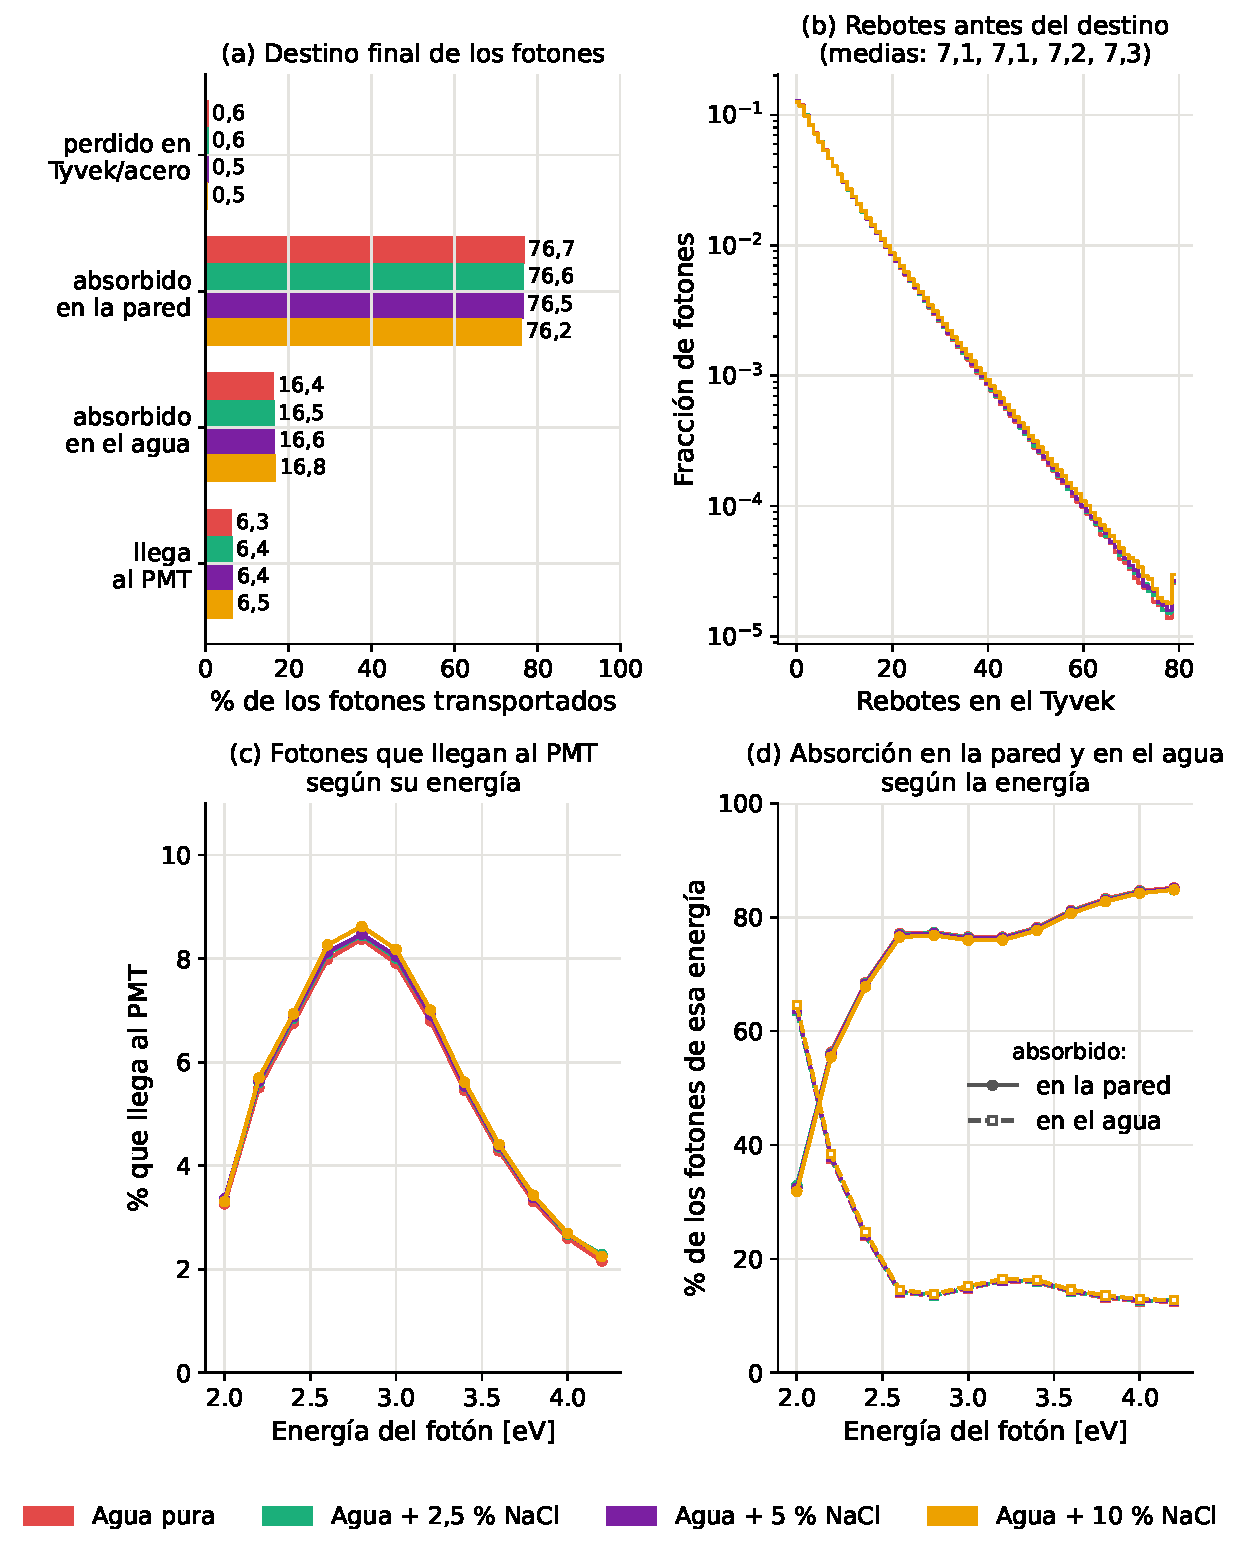
\includegraphics[width=\linewidth]{fig07_destino_fotones.pdf}
			\vspace{0.2cm}
			\captionsetup{width=\textwidth,justification=justified,singlelinecheck=false}
			\caption[Destino de los fotones Cherenkov transportados]{Destino de los fotones Cherenkov transportados en \textcolor{red}{agua pura}, \textcolor{green}{agua + 2.5\,\% de NaCl}, \textcolor{violet}{agua + 5\,\% de NaCl} y \textcolor{orange}{agua + 10\,\% de NaCl}: (a) destino final; (b) número de reflexiones en el Tyvek antes del destino; (c) fracción que llega al PMT según la energía del fotón; (d) fracción absorbida en la pared (línea continua) y en el agua (línea discontinua) según la energía.}
			\label{fig:destino-fotones}
		\end{minipage}
	\end{adjustwidth}
\end{figure}

\paragraph{Histograma de carga:} La Figura~(\ref{Num-pho}) muestra el histograma de carga en el PMT, aporte de este trabajo respecto al de referencia. El 53\,\% de los neutrones deja al menos un fotoelectrón; la mediana es 1~p.e. y la media 9.8~p.e. en \textcolor{red}{agua pura}, y solo el 2.5\,\% de los eventos supera 100~p.e. La carga media aumenta un 16.4\,\% (\textcolor{green}{2.5\,\%}), un 27.0\,\% (\textcolor{violet}{5\,\%}) y un 42.0\,\% (\textcolor{orange}{10\,\%}) respecto al agua pura, y la fracción de la carga asociada a las capturas (1~µs--1~ms) pasa del 12.7\,\% al 22.9\,\%, 26.9\,\% y 31.1\,\%. El transporte óptico es prácticamente el mismo en todos los medios (Figura~\ref{fig:destino-fotones}): llega al PMT entre el 6.30 y el 6.50\,\% de los fotones transportados, se absorbe en la pared el 76.2--76.7\,\% y en el agua el 16.4--16.8\,\%, con 7.1--7.3 reflexiones medias y la misma dependencia con la energía del fotón, de modo que el modelo del Tyvek fija una escala común de la carga pero no altera las diferencias entre medios. Su escala absoluta depende del modelo óptico (Tabla~\ref{tab:sensibilidad-tyvek}).

\begin{figure}[!htbp]
	\begin{adjustwidth}{0cm}{0cm}
		\centering
		\begin{minipage}{\linewidth}
			\centering
			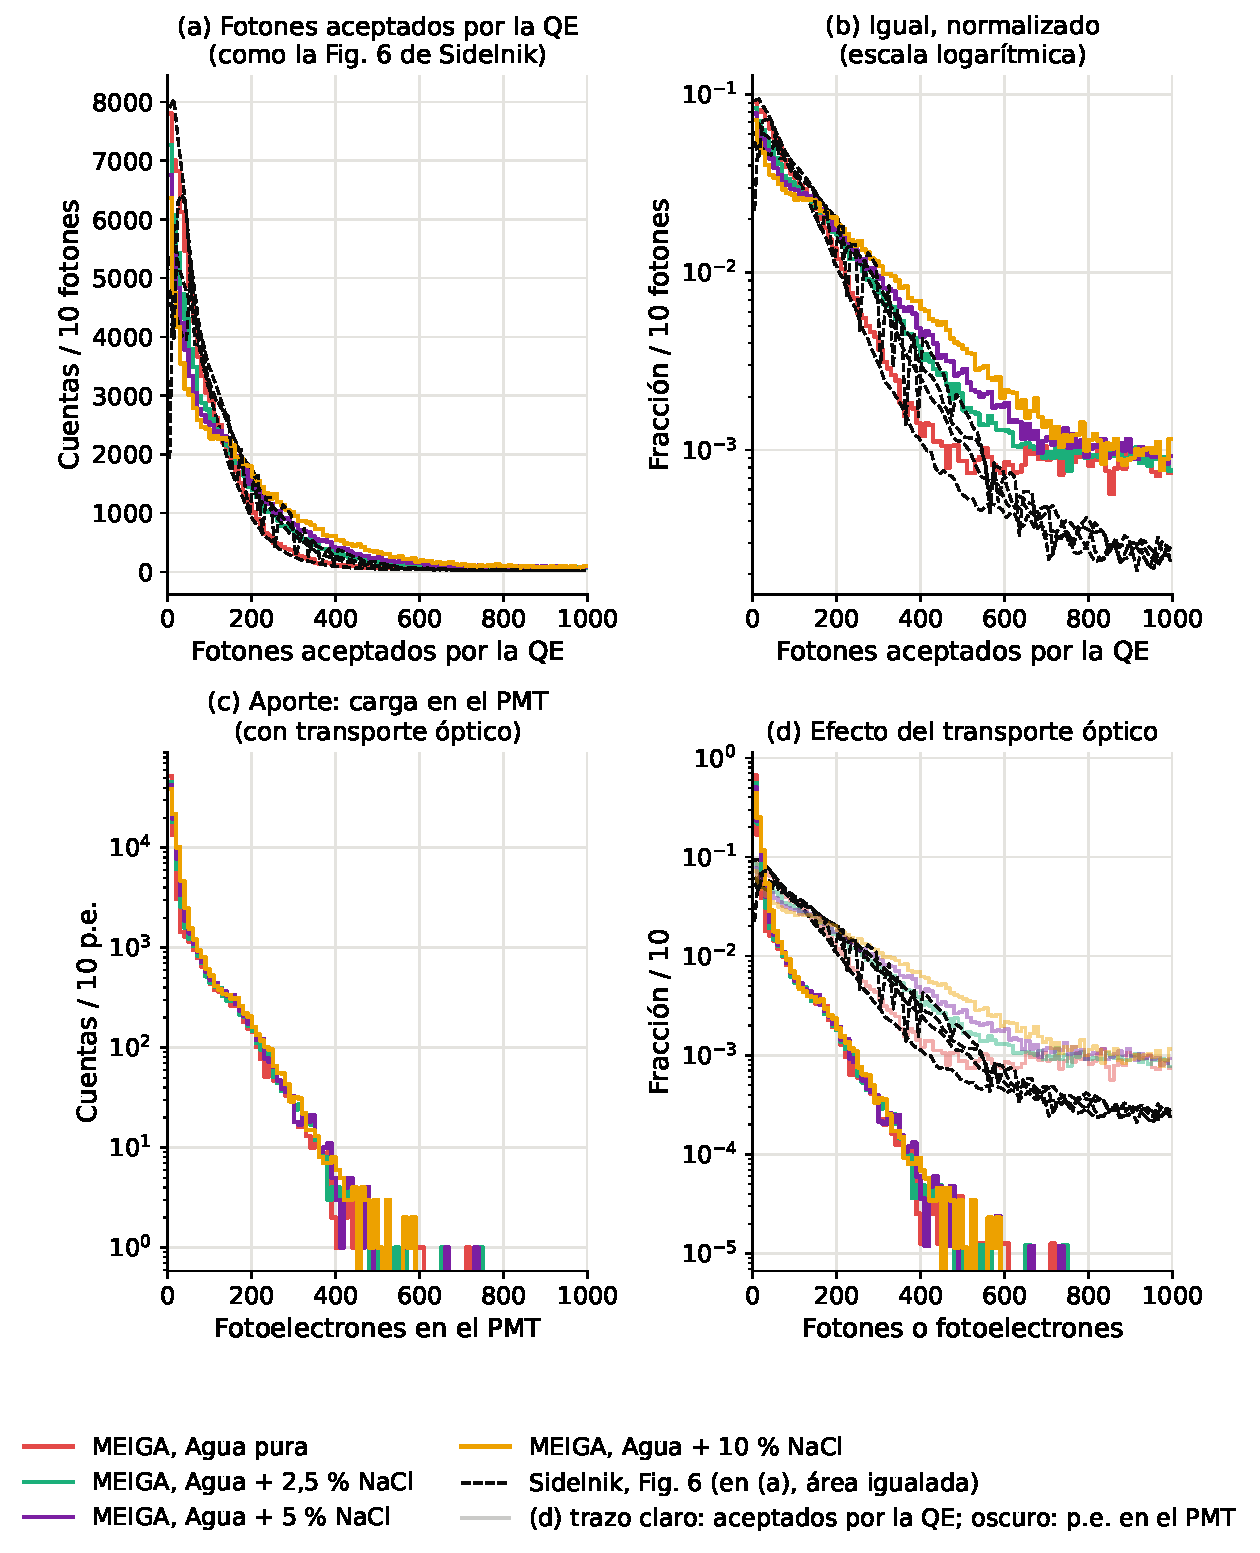
\includegraphics[width=\linewidth]{fig09_histograma_tipo_sidelnik.pdf}
			\vspace{0.2cm}
			\captionsetup{width=\textwidth,justification=justified,singlelinecheck=false}
			\caption[Histograma de carga del WCD para neutrones de 500~MeV]{(a, b) Fotones aceptados por la eficiencia cuántica antes del transporte óptico, frente a la Fig.~6 de \protect\citet{Sidelnik2020} (área igualada y normalizado, en escala logarítmica). (c) Histograma de carga en el PMT, con transporte óptico. (d) Efecto del transporte óptico: fotones aceptados frente a fotoelectrones. Eventos con al menos un fotón o fotoelectrón; $1.5\times10^{5}$ neutrones de 500~MeV por medio.}
			\label{Num-pho}
		\end{minipage}
	\end{adjustwidth}
\end{figure}

%==========================================================
\section{Síntesis de la validación}
\label{subsubsec:sintesis-validacion}
%==========================================================

La Tabla~(\ref{tab:sintesis-validacion}) resume el resultado de la validación para cada eslabón de la cadena de procesos, según los tres niveles de comparación definidos en la introducción (Sec.~\ref{sec:Res-WCD-500MeV}).

\begin{table}[!htbp]
	\centering
	\small
	\captionsetup{width=\linewidth,justification=justified,singlelinecheck=false}
	\caption[Síntesis de la validación del modelo frente a Sidelnik et al. (2020)]{Síntesis de la validación del modelo Monte Carlo frente a \protect\citet{Sidelnik2020}. Nivel: (i) valor absoluto; (ii) cociente o forma normalizada; (iii) tendencia con la concentración de NaCl.}
	\label{tab:sintesis-validacion}
	\renewcommand{\arraystretch}{1.2}
	\begin{tabularx}{\linewidth}{>{\raggedright\arraybackslash}p{0.24\linewidth} >{\centering\arraybackslash}p{0.06\linewidth} >{\raggedright\arraybackslash}X >{\centering\arraybackslash}p{0.16\linewidth}}
		\toprule
		\textbf{Observable} & \textbf{Nivel} & \textbf{Resultado} & \textbf{Concordancia} \\
		\midrule
		Moderación (elásticas) & (i) & $\xi_{\mathrm{H}}=1.000$, $\xi_{\mathrm{O}}=0.118$ (teoría 0.121); la sal no modifica la moderación & Completa \\
		Probabilidad de captura & (i) & 24.08\,\% frente a 25.18\,\% en agua pura & Buena \\
		 & (iii) & Mismo signo y monótono; aumento con NaCl $\approx$\,2 veces menor (+8.3\,\% frente a +16.2\,\% con 10\,\%) & Parcial \\
		Tiempo de captura & (i) & 192 / 140 / 109 / 75~µs frente a 205 / 147 / 114 / 78~µs (teoría) & Buena \\
		Distancia de captura & (iii) & Disminuye con NaCl si se mide desde el vértice del neutrón & Cualitativa \\
		Líneas gamma de captura & (i) & Energías e intensidades por captura; gamma único de $S_n$ en $\approx$\,24\,\% de las capturas & Buena, con limitación \\
		Espectro gamma & (ii) & 6.13/2.223 = 0.022 en ambos; líneas del Cl dentro del 3--10\,\%; exceso en 0.511 y 8.58~MeV & Buena, con diferencias explicadas \\
		Espectro de electrones & (i) & Escala absoluta (cociente 1.06) y bordes Compton & Muy buena \\
		Deuterones de captura & (i) & Mediana 1.319~keV (cinemática: 1.319~keV) & Completa \\
		Fotones aceptados (Fig.~6) & (i) & Coincidencia sin reescalar entre 0 y 500 fotones; cola de piones mayor & Buena hasta 500 fotones \\
		Efecto del NaCl en la luz & (iii) & Curvas de razón: $r=0.88$--$0.91$ en los tres medios con NaCl; razón media 100--500 dentro del 1\,\% con 2.5 y 5\,\% & Alta \\
		\bottomrule
	\end{tabularx}
\end{table}

En conjunto, el modelo reproduce la física de moderación y captura del detector de referencia, el campo gamma de captura y su conversión en electrones, la producción de luz Cherenkov y, sobre todo, el efecto relativo del NaCl en la señal. Las diferencias identificadas tienen un origen físico concreto: (i) la mayor producción de piones del modelo de Bertini a 500~MeV, que forma la cola de la distribución de fotones por encima de 500 y que no afecta a la región de captura; (ii) una mayor producción de gammas de desexcitación nuclear tras la dispersión inelástica de neutrones, que eleva el fondo y diluye parcialmente el efecto del Cl; y (iii) el modelo de captura de \textsc{Geant4}, que no conserva la energía en las cascadas del Cl y emite un gamma único con toda la energía de separación en una cuarta parte de las capturas. Esta última limitación sobreestima la luz de las capturas en Cl y debe tenerse en cuenta en la interpretación de la respuesta absoluta del detector a neutrones en los medios con NaCl.


\appendix
% ARCHIVO GENERADO por scripts/construir_informe.py a partir de apendice_procesos.tex: no editar aqui.
% Apendice generado a partir de informe/Informe-Sidelnik-500MeV.tex (tablas de canales_reaccion.py), con punto decimal.
\section{Ecuaciones, energías y porcentajes de los procesos de los neutrones de 500~MeV}
\label{ap:procesos-neutrones}

Las Tablas~\ref{tab:procesos_pura}--\ref{tab:procesos_nacl10} reúnen, para cada medio simulado en la Sec.~\ref{sec:Res-WCD-500MeV}, todas las reacciones de los neutrones en el volumen del detector (primario y secundarios): la ecuación de la reacción, el valor $Q$ del estado fundamental (calculado con los excesos de masa de la evaluación AME2020; $Q<0$ es la energía umbral que se gasta en romper el núcleo), la energía típica del neutrón incidente (mediana y, entre paréntesis, la fracción de reacciones por debajo de 20~MeV), el porcentaje dentro de cada tipo de proceso y los gammas que emite. El núcleo blanco de cada interacción inelástica se deduce por conservación de la carga y del número bariónico de los productos. En las inelásticas, las líneas $\gamma$ solo se atribuyen si pertenecen al núcleo residual o al blanco de esa misma reacción (ventana de $\pm10$~keV); se listan los canales con más del 0.4\,\% de las inelásticas y, en los medios con NaCl, también los del Na y el Cl.

Estas tablas explican el origen de los gammas y, por tanto, de los electrones y de la luz Cherenkov: la dispersión elástica en $^{1}$H modera los neutrones ($\xi=1$); la captura en $^{1}$H y en $^{35}$Cl produce los gammas de captura; y las interacciones inelásticas en $^{16}$O producen el fondo de desexcitación nuclear (líneas de 4.44, 6.13, 6.92 y 7.12~MeV y un continuo) y los núcleos emisores $\beta^{+}$ ($^{15}$O, $^{13}$N, $^{11}$C) responsables de la línea de aniquilación de larga vida.

\clearpage
{\footnotesize\setlength{\tabcolsep}{4pt}\setlength{\LTpre}{0pt}
\begin{longtable}{@{}>{\raggedright\arraybackslash}p{3.3cm}>{\raggedleft\arraybackslash}p{1.35cm}>{\raggedleft\arraybackslash}p{3.4cm}>{\raggedleft\arraybackslash}p{1.3cm}>{\raggedright\arraybackslash}p{\dimexpr\linewidth-9.35cm-8\tabcolsep\relax}@{}}
\captionsetup{width=\linewidth}\caption[Procesos de los neutrones: Agua pura]{\textcolor{red}{Agua pura}: ecuaciones, energías y porcentajes de los procesos de los neutrones (150\,000 neutrones de 500\,MeV).}\label{tab:procesos_pura}\\\toprule
Reacción & $Q$ (MeV) & $E_n$ típica & \% & Gammas emitidos (keV) \\\midrule\endfirsthead
\toprule Reacción & $Q$ (MeV) & $E_n$ típica & \% & Gammas emitidos (keV) \\\midrule\endhead
\multicolumn{5}{@{}>{\raggedright\arraybackslash}p{\linewidth}@{}}{\textbf{Dispersión elástica} (104 por neutrón incidente; \% de las colisiones con blanco reconstruido, $E>1$\,eV)}\\
$^1$H(n,n)$^1$H & 0 & todas & 83.74\,\% & pierde 0--100\,\% de $E$; $\xi = 1.00$ \\
$^{16}$O(n,n)$^{16}$O & 0 & todas & 15.95\,\% & pierde 0--22\,\%; $\xi = 0.12$ ($<$\,1\,MeV) \\
\midrule\multicolumn{5}{@{}>{\raggedright\arraybackslash}p{\linewidth}@{}}{\textbf{Captura radiativa} (0.829 por neutrón incidente; \% de las capturas en el agua)}\\
$^1$H(n,$\gamma$)$^2$H & +2.225 & térmica & 99.94\,\% & 2224 (MEIGA: 2224.4) \\
$^{16}$O(n,$\gamma$)$^{17}$O & +4.143 & térmica & 0.06\,\% & 871, 1088, 2184; $\gamma$ único 4143 \\
\midrule\multicolumn{5}{@{}>{\raggedright\arraybackslash}p{\linewidth}@{}}{\textbf{Inelástica} (1.29 por neutrón incidente; \% de las inelásticas; canales con más del 0.4\,\%)}\\
$^{16}$O(n,np)$^{15}$N & -12.13 & 354\,MeV & 12.9\,\% & 2.2 $\gamma$/reacc.; continuo \\
$^{16}$O(n,n')$^{16}$O & 0.00 & 21\,MeV (48\,\% $<$\,20) & 11.3\,\% & 2.8 $\gamma$/reacc.; 6130 (14\,\%), 7117 (6\,\%), 2741 (4\,\%) \\
$^{16}$O(n,n$\alpha$)$^{12}$C & -7.16 & 39\,MeV (16\,\% $<$\,20) & 9.5\,\% & 1.7 $\gamma$/reacc.; 4439 (6\,\%) \\
$^{16}$O(n,2n)$^{15}$O & -15.66 & 500\,MeV & 9.4\,\% & 2.1 $\gamma$/reacc.; continuo \\
$^{16}$O(n,2np)$^{14}$N & -22.96 & 377\,MeV & 9.1\,\% & 2.0 $\gamma$/reacc.; continuo \\
$^{16}$O(n,3n2p)$^{12}$C & -35.46 & 500\,MeV & 6.7\,\% & 2.1 $\gamma$/reacc.; continuo \\
$^{16}$O(n,2n2p)$^{13}$C & -30.51 & 477\,MeV & 4.0\,\% & 1.7 $\gamma$/reacc.; continuo \\
$^{16}$O(n,$\alpha$)$^{13}$C & -2.22 & 10\,MeV (100\,\% $<$\,20) & 3.1\,\% & 2.4 $\gamma$/reacc.; continuo \\
$^{16}$O(n,n2p)$^{14}$C & -22.33 & 384\,MeV & 2.9\,\% & 2.1 $\gamma$/reacc.; continuo \\
$^{16}$O(n,3n2p$\alpha$)$^{8}$Be & -42.82 & 500\,MeV & 2.1\,\% & 1.6 $\gamma$/reacc.; continuo \\
$^{16}$O(n,2npd)$^{12}$C & -33.23 & 380\,MeV & 1.9\,\% & 2.2 $\gamma$/reacc.; continuo \\
$^{16}$O(n,3n2p3$\alpha$) & -42.73 & 500\,MeV & 1.4\,\% & 1.7 $\gamma$/reacc.; continuo \\
$^{16}$O(n,3np)$^{13}$N & -33.51 & 500\,MeV & 1.1\,\% & 1.6 $\gamma$/reacc.; continuo \\
$^{16}$O(n,n2$\alpha$)$^{8}$Be & -14.53 & 68\,MeV & 1.0\,\% & 1.5 $\gamma$/reacc.; continuo \\
$^{16}$O(n,3n3p)$^{11}$B & -51.41 & 500\,MeV & 0.8\,\% & 2.3 $\gamma$/reacc.; continuo \\
$^{16}$O(n,np$\pi^-$)$^{15}$O & -154.45 & 500\,MeV & 0.7\,\% & 2.3 $\gamma$/reacc.; continuo \\
$^{16}$O(n,p)$^{16}$N & -9.64 & 19\,MeV (54\,\% $<$\,20) & 0.7\,\% & 2.0 $\gamma$/reacc.; continuo \\
$^{1}$H(n,np$\pi^0$) & -134.98 & 500\,MeV & 0.7\,\% & 0.0 $\gamma$/reacc.; sin $\gamma$ directos \\
$^{16}$O(n,2npd$\alpha$)$^{8}$Be & -40.60 & 500\,MeV & 0.7\,\% & 1.6 $\gamma$/reacc.; continuo \\
$^{16}$O(n,3n)$^{14}$O & -28.89 & 500\,MeV & 0.7\,\% & 2.1 $\gamma$/reacc.; continuo \\
$^{16}$O(n,np$\pi^0$)$^{15}$N & -147.10 & 500\,MeV & 0.6\,\% & 2.6 $\gamma$/reacc.; continuo \\
$^{16}$O(n,4n3pd2$\alpha$) & -68.80 & 500\,MeV & 0.5\,\% & 2.0 $\gamma$/reacc.; continuo \\
$^{16}$O(n,4n3p)$^{10}$B & -62.87 & 500\,MeV & 0.5\,\% & 1.8 $\gamma$/reacc.; continuo \\
$^{16}$O(n,5n4p2$\alpha$) & -71.03 & 500\,MeV & 0.5\,\% & 1.9 $\gamma$/reacc.; continuo \\
$^{16}$O(n,2n3p$\pi^-$)$^{12}$C & -174.25 & 500\,MeV & 0.5\,\% & 2.1 $\gamma$/reacc.; continuo \\
$^{16}$O(n,4n2p)$^{11}$C & -54.18 & 500\,MeV & 0.5\,\% & 2.2 $\gamma$/reacc.; continuo \\
$^{16}$O(n,n2p$\pi^-$)$^{14}$N & -161.75 & 500\,MeV & 0.4\,\% & 2.0 $\gamma$/reacc.; continuo \\
$^{16}$O(n,2npd3$\alpha$) & -40.51 & 500\,MeV & 0.4\,\% & 1.6 $\gamma$/reacc.; continuo \\
$^{16}$O(n,3n2p$\pi^0$)$^{12}$C & -170.43 & 500\,MeV & 0.4\,\% & 2.2 $\gamma$/reacc.; continuo \\
\bottomrule\end{longtable}}
\clearpage
{\footnotesize\setlength{\tabcolsep}{4pt}\setlength{\LTpre}{0pt}
\begin{longtable}{@{}>{\raggedright\arraybackslash}p{3.3cm}>{\raggedleft\arraybackslash}p{1.35cm}>{\raggedleft\arraybackslash}p{3.4cm}>{\raggedleft\arraybackslash}p{1.3cm}>{\raggedright\arraybackslash}p{\dimexpr\linewidth-9.35cm-8\tabcolsep\relax}@{}}
\captionsetup{width=\linewidth}\caption[Procesos de los neutrones: 2.5\,\% NaCl]{\textcolor{green}{Agua + 2.5\,\% NaCl}: ecuaciones, energías y porcentajes de los procesos de los neutrones (150\,000 neutrones de 500\,MeV).}\label{tab:procesos_nacl25}\\\toprule
Reacción & $Q$ (MeV) & $E_n$ típica & \% & Gammas emitidos (keV) \\\midrule\endfirsthead
\toprule Reacción & $Q$ (MeV) & $E_n$ típica & \% & Gammas emitidos (keV) \\\midrule\endhead
\multicolumn{5}{@{}>{\raggedright\arraybackslash}p{\linewidth}@{}}{\textbf{Dispersión elástica} (83 por neutrón incidente; \% de las colisiones con blanco reconstruido, $E>1$\,eV)}\\
$^1$H(n,n)$^1$H & 0 & todas & 83.55\,\% & pierde 0--100\,\% de $E$; $\xi = 1.00$ \\
$^{16}$O(n,n)$^{16}$O & 0 & todas & 15.82\,\% & pierde 0--22\,\%; $\xi = 0.12$ ($<$\,1\,MeV) \\
$^{23}$Na(n,n)$^{23}$Na & 0 & todas & 0.47\,\% & pierde 0--16\,\% \\
$^{35.37}$Cl(n,n)$^{35.37}$Cl & 0 & todas & 0.16\,\% & pierde 0--11\,\% \\
\midrule\multicolumn{5}{@{}>{\raggedright\arraybackslash}p{\linewidth}@{}}{\textbf{Captura radiativa} (0.864 por neutrón incidente; \% de las capturas en el agua)}\\
$^1$H(n,$\gamma$)$^2$H & +2.225 & térmica & 63.53\,\% & 2224 (MEIGA: 2224.4) \\
$^{35}$Cl(n,$\gamma$)$^{36}$Cl & +8.580 & térmica & 35.75\,\% & 517, 788, 1165, 1951, 6111, 7414; $\gamma$ único 8580 \\
$^{23}$Na(n,$\gamma$)$^{24}$Na & +6.959 & térmica & 0.57\,\% & 472 (0.9\,\%); $\gamma$ único 6959 \\
$^{37}$Cl(n,$\gamma$)$^{38}$Cl & +6.108 & térmica & 0.11\,\% & 638, 755, 1692; $\gamma$ único 6108 \\
$^{16}$O(n,$\gamma$)$^{17}$O & +4.143 & térmica & 0.03\,\% & 871, 1088, 2184; $\gamma$ único 4143 \\
\midrule\multicolumn{5}{@{}>{\raggedright\arraybackslash}p{\linewidth}@{}}{\textbf{Inelástica} (1.33 por neutrón incidente; \% de las inelásticas; canales con más del 0.4\,\% y los del Na y el Cl)}\\
$^{16}$O(n,np)$^{15}$N & -12.13 & 350\,MeV & 12.6\,\% & 2.2 $\gamma$/reacc.; continuo \\
$^{16}$O(n,n')$^{16}$O & 0.00 & 21\,MeV (49\,\% $<$\,20) & 11.0\,\% & 2.8 $\gamma$/reacc.; 6130 (14\,\%), 7117 (6\,\%), 6917 (4\,\%) \\
$^{16}$O(n,n$\alpha$)$^{12}$C & -7.16 & 39\,MeV (16\,\% $<$\,20) & 9.3\,\% & 1.7 $\gamma$/reacc.; 4439 (6\,\%) \\
$^{16}$O(n,2n)$^{15}$O & -15.66 & 500\,MeV & 9.0\,\% & 2.1 $\gamma$/reacc.; continuo \\
$^{16}$O(n,2np)$^{14}$N & -22.96 & 373\,MeV & 8.8\,\% & 2.0 $\gamma$/reacc.; continuo \\
$^{16}$O(n,3n2p)$^{12}$C & -35.46 & 500\,MeV & 6.4\,\% & 2.1 $\gamma$/reacc.; continuo \\
$^{16}$O(n,2n2p)$^{13}$C & -30.51 & 471\,MeV & 4.0\,\% & 1.7 $\gamma$/reacc.; continuo \\
$^{16}$O(n,$\alpha$)$^{13}$C & -2.22 & 10\,MeV (100\,\% $<$\,20) & 3.1\,\% & 2.4 $\gamma$/reacc.; continuo \\
$^{16}$O(n,n2p)$^{14}$C & -22.33 & 406\,MeV & 2.8\,\% & 2.0 $\gamma$/reacc.; continuo \\
$^{16}$O(n,3n2p$\alpha$)$^{8}$Be & -42.82 & 500\,MeV & 2.0\,\% & 1.6 $\gamma$/reacc.; continuo \\
$^{16}$O(n,2npd)$^{12}$C & -33.23 & 399\,MeV & 1.8\,\% & 2.2 $\gamma$/reacc.; continuo \\
$^{16}$O(n,3n2p3$\alpha$) & -42.73 & 500\,MeV & 1.5\,\% & 1.7 $\gamma$/reacc.; continuo \\
$^{16}$O(n,3np)$^{13}$N & -33.51 & 500\,MeV & 1.1\,\% & 1.7 $\gamma$/reacc.; continuo \\
$^{16}$O(n,n2$\alpha$)$^{8}$Be & -14.53 & 70\,MeV & 1.0\,\% & 1.5 $\gamma$/reacc.; continuo \\
$^{16}$O(n,3n3p)$^{11}$B & -51.41 & 500\,MeV & 0.8\,\% & 2.3 $\gamma$/reacc.; continuo \\
$^{16}$O(n,np$\pi^-$)$^{15}$O & -154.45 & 500\,MeV & 0.7\,\% & 2.3 $\gamma$/reacc.; continuo \\
$^{16}$O(n,p)$^{16}$N & -9.64 & 19\,MeV (54\,\% $<$\,20) & 0.7\,\% & 2.0 $\gamma$/reacc.; continuo \\
$^{16}$O(n,3n)$^{14}$O & -28.89 & 500\,MeV & 0.6\,\% & 2.2 $\gamma$/reacc.; continuo \\
$^{1}$H(n,np$\pi^0$) & -134.98 & 500\,MeV & 0.6\,\% & 0.0 $\gamma$/reacc.; sin $\gamma$ directos \\
$^{16}$O(n,2npd$\alpha$)$^{8}$Be & -40.60 & 472\,MeV & 0.6\,\% & 1.6 $\gamma$/reacc.; continuo \\
$^{16}$O(n,np$\pi^0$)$^{15}$N & -147.10 & 500\,MeV & 0.6\,\% & 2.7 $\gamma$/reacc.; continuo \\
$^{16}$O(n,4n3pd2$\alpha$) & -68.80 & 500\,MeV & 0.5\,\% & 1.9 $\gamma$/reacc.; continuo \\
$^{16}$O(n,4n3p)$^{10}$B & -62.87 & 500\,MeV & 0.5\,\% & 1.8 $\gamma$/reacc.; continuo \\
$^{16}$O(n,2n3p$\pi^-$)$^{12}$C & -174.25 & 500\,MeV & 0.5\,\% & 2.2 $\gamma$/reacc.; continuo \\
$^{16}$O(n,5n4p2$\alpha$) & -71.03 & 500\,MeV & 0.5\,\% & 1.9 $\gamma$/reacc.; continuo \\
$^{16}$O(n,4n2p)$^{11}$C & -54.18 & 500\,MeV & 0.5\,\% & 2.2 $\gamma$/reacc.; continuo \\
$^{16}$O(n,n2p$\pi^-$)$^{14}$N & -161.75 & 500\,MeV & 0.4\,\% & 2.0 $\gamma$/reacc.; continuo \\
$^{23}$Na(n,n')$^{23}$Na & 0.00 & 7\,MeV (85\,\% $<$\,20) & 0.3\,\% & 2.6 $\gamma$/reacc.; 440 (74\,\%) \\
$^{35}$Cl(n,p)$^{35}$S & 0.62 & térmica (96\,\% $<$\,20) & 0.3\,\% & 0.4 $\gamma$/reacc.; continuo \\
\bottomrule\end{longtable}}
\clearpage
{\footnotesize\setlength{\tabcolsep}{4pt}\setlength{\LTpre}{0pt}
\begin{longtable}{@{}>{\raggedright\arraybackslash}p{3.3cm}>{\raggedleft\arraybackslash}p{1.35cm}>{\raggedleft\arraybackslash}p{3.4cm}>{\raggedleft\arraybackslash}p{1.3cm}>{\raggedright\arraybackslash}p{\dimexpr\linewidth-9.35cm-8\tabcolsep\relax}@{}}
\captionsetup{width=\linewidth}\caption[Procesos de los neutrones: 5\,\% NaCl]{\textcolor{violet}{Agua + 5\,\% NaCl}: ecuaciones, energías y porcentajes de los procesos de los neutrones (150\,000 neutrones de 500\,MeV).}\label{tab:procesos_nacl5}\\\toprule
Reacción & $Q$ (MeV) & $E_n$ típica & \% & Gammas emitidos (keV) \\\midrule\endfirsthead
\toprule Reacción & $Q$ (MeV) & $E_n$ típica & \% & Gammas emitidos (keV) \\\midrule\endhead
\multicolumn{5}{@{}>{\raggedright\arraybackslash}p{\linewidth}@{}}{\textbf{Dispersión elástica} (72 por neutrón incidente; \% de las colisiones con blanco reconstruido, $E>1$\,eV)}\\
$^1$H(n,n)$^1$H & 0 & todas & 83.33\,\% & pierde 0--100\,\% de $E$; $\xi = 1.00$ \\
$^{16}$O(n,n)$^{16}$O & 0 & todas & 15.71\,\% & pierde 0--22\,\%; $\xi = 0.12$ ($<$\,1\,MeV) \\
$^{23}$Na(n,n)$^{23}$Na & 0 & todas & 0.68\,\% & pierde 0--16\,\% \\
$^{35.37}$Cl(n,n)$^{35.37}$Cl & 0 & todas & 0.28\,\% & pierde 0--11\,\% \\
\midrule\multicolumn{5}{@{}>{\raggedright\arraybackslash}p{\linewidth}@{}}{\textbf{Captura radiativa} (0.903 por neutrón incidente; \% de las capturas en el agua)}\\
$^{35}$Cl(n,$\gamma$)$^{36}$Cl & +8.580 & térmica & 51.47\,\% & 517, 788, 1165, 1951, 6111, 7414; $\gamma$ único 8580 \\
$^1$H(n,$\gamma$)$^2$H & +2.225 & térmica & 47.53\,\% & 2224 (MEIGA: 2224.4) \\
$^{23}$Na(n,$\gamma$)$^{24}$Na & +6.959 & térmica & 0.80\,\% & 472 (0.9\,\%); $\gamma$ único 6959 \\
$^{37}$Cl(n,$\gamma$)$^{38}$Cl & +6.108 & térmica & 0.17\,\% & 638, 755, 1692; $\gamma$ único 6108 \\
$^{16}$O(n,$\gamma$)$^{17}$O & +4.143 & térmica & 0.03\,\% & 871, 1088, 2184; $\gamma$ único 4143 \\
\midrule\multicolumn{5}{@{}>{\raggedright\arraybackslash}p{\linewidth}@{}}{\textbf{Inelástica} (1.36 por neutrón incidente; \% de las inelásticas; canales con más del 0.4\,\% y los del Na y el Cl)}\\
$^{16}$O(n,np)$^{15}$N & -12.13 & 326\,MeV & 12.1\,\% & 2.2 $\gamma$/reacc.; continuo \\
$^{16}$O(n,n')$^{16}$O & 0.00 & 20\,MeV (50\,\% $<$\,20) & 10.8\,\% & 2.8 $\gamma$/reacc.; 6130 (14\,\%), 7117 (6\,\%), 6917 (4\,\%) \\
$^{16}$O(n,n$\alpha$)$^{12}$C & -7.16 & 38\,MeV (16\,\% $<$\,20) & 9.2\,\% & 1.7 $\gamma$/reacc.; 4439 (6\,\%) \\
$^{16}$O(n,2n)$^{15}$O & -15.66 & 500\,MeV & 8.7\,\% & 2.1 $\gamma$/reacc.; continuo \\
$^{16}$O(n,2np)$^{14}$N & -22.96 & 352\,MeV & 8.7\,\% & 2.0 $\gamma$/reacc.; continuo \\
$^{16}$O(n,3n2p)$^{12}$C & -35.46 & 500\,MeV & 6.2\,\% & 2.1 $\gamma$/reacc.; continuo \\
$^{16}$O(n,2n2p)$^{13}$C & -30.51 & 465\,MeV & 3.8\,\% & 1.7 $\gamma$/reacc.; continuo \\
$^{16}$O(n,$\alpha$)$^{13}$C & -2.22 & 10\,MeV (100\,\% $<$\,20) & 3.0\,\% & 2.4 $\gamma$/reacc.; continuo \\
$^{16}$O(n,n2p)$^{14}$C & -22.33 & 354\,MeV & 2.7\,\% & 2.1 $\gamma$/reacc.; continuo \\
$^{16}$O(n,3n2p$\alpha$)$^{8}$Be & -42.82 & 500\,MeV & 2.0\,\% & 1.6 $\gamma$/reacc.; continuo \\
$^{16}$O(n,2npd)$^{12}$C & -33.23 & 362\,MeV & 1.8\,\% & 2.2 $\gamma$/reacc.; continuo \\
$^{16}$O(n,3n2p3$\alpha$) & -42.73 & 500\,MeV & 1.4\,\% & 1.7 $\gamma$/reacc.; continuo \\
$^{16}$O(n,3np)$^{13}$N & -33.51 & 500\,MeV & 1.1\,\% & 1.6 $\gamma$/reacc.; continuo \\
$^{16}$O(n,n2$\alpha$)$^{8}$Be & -14.53 & 71\,MeV & 1.0\,\% & 1.5 $\gamma$/reacc.; continuo \\
$^{16}$O(n,3n3p)$^{11}$B & -51.41 & 500\,MeV & 0.7\,\% & 2.3 $\gamma$/reacc.; continuo \\
$^{16}$O(n,np$\pi^-$)$^{15}$O & -154.45 & 500\,MeV & 0.6\,\% & 2.3 $\gamma$/reacc.; continuo \\
$^{16}$O(n,2npd$\alpha$)$^{8}$Be & -40.60 & 487\,MeV & 0.6\,\% & 1.6 $\gamma$/reacc.; continuo \\
$^{16}$O(n,p)$^{16}$N & -9.64 & 18\,MeV (55\,\% $<$\,20) & 0.6\,\% & 1.9 $\gamma$/reacc.; continuo \\
$^{1}$H(n,np$\pi^0$) & -134.98 & 500\,MeV & 0.6\,\% & 0.0 $\gamma$/reacc.; sin $\gamma$ directos \\
$^{16}$O(n,3n)$^{14}$O & -28.89 & 500\,MeV & 0.6\,\% & 2.1 $\gamma$/reacc.; continuo \\
$^{16}$O(n,np$\pi^0$)$^{15}$N & -147.10 & 500\,MeV & 0.5\,\% & 2.6 $\gamma$/reacc.; continuo \\
$^{23}$Na(n,n')$^{23}$Na & 0.00 & 7\,MeV (84\,\% $<$\,20) & 0.5\,\% & 2.5 $\gamma$/reacc.; 440 (72\,\%), 2076 (2\,\%) \\
$^{16}$O(n,4n3pd2$\alpha$) & -68.80 & 500\,MeV & 0.5\,\% & 1.9 $\gamma$/reacc.; continuo \\
$^{16}$O(n,4n2p)$^{11}$C & -54.18 & 500\,MeV & 0.5\,\% & 2.2 $\gamma$/reacc.; continuo \\
$^{16}$O(n,4n3p)$^{10}$B & -62.87 & 500\,MeV & 0.5\,\% & 1.8 $\gamma$/reacc.; continuo \\
$^{35}$Cl(n,p)$^{35}$S & 0.62 & térmica (96\,\% $<$\,20) & 0.5\,\% & 0.5 $\gamma$/reacc.; continuo \\
$^{16}$O(n,5n4p2$\alpha$) & -71.03 & 500\,MeV & 0.4\,\% & 1.9 $\gamma$/reacc.; continuo \\
$^{16}$O(n,2n3p$\pi^-$)$^{12}$C & -174.25 & 500\,MeV & 0.4\,\% & 2.2 $\gamma$/reacc.; continuo \\
$^{16}$O(n,n2p$\pi^-$)$^{14}$N & -161.75 & 500\,MeV & 0.4\,\% & 2.1 $\gamma$/reacc.; continuo \\
$^{23}$Na(n,np)$^{22}$Ne & -8.79 & 155\,MeV & 0.3\,\% & 2.2 $\gamma$/reacc.; continuo \\
$^{35}$Cl(n,np)$^{34}$S & -6.37 & 122\,MeV & 0.3\,\% & 2.5 $\gamma$/reacc.; continuo \\
$^{35}$Cl(n,n')$^{35}$Cl & 0.00 & 7\,MeV (77\,\% $<$\,20) & 0.3\,\% & 2.4 $\gamma$/reacc.; 1219 (18\,\%), 1763 (10\,\%) \\
$^{23}$Na(n,2np)$^{21}$Ne & -19.16 & 211\,MeV & 0.2\,\% & 2.0 $\gamma$/reacc.; 440 (3\,\%) \\
$^{35}$Cl(n,2np)$^{33}$S & -17.79 & 247\,MeV & 0.2\,\% & 2.1 $\gamma$/reacc.; continuo \\
\bottomrule\end{longtable}}
\clearpage
{\footnotesize\setlength{\tabcolsep}{4pt}\setlength{\LTpre}{0pt}
\begin{longtable}{@{}>{\raggedright\arraybackslash}p{3.3cm}>{\raggedleft\arraybackslash}p{1.35cm}>{\raggedleft\arraybackslash}p{3.4cm}>{\raggedleft\arraybackslash}p{1.3cm}>{\raggedright\arraybackslash}p{\dimexpr\linewidth-9.35cm-8\tabcolsep\relax}@{}}
\captionsetup{width=\linewidth}\caption[Procesos de los neutrones: 10\,\% NaCl]{\textcolor{orange}{Agua + 10\,\% NaCl}: ecuaciones, energías y porcentajes de los procesos de los neutrones (150\,000 neutrones de 500\,MeV).}\label{tab:procesos_nacl10}\\\toprule
Reacción & $Q$ (MeV) & $E_n$ típica & \% & Gammas emitidos (keV) \\\midrule\endfirsthead
\toprule Reacción & $Q$ (MeV) & $E_n$ típica & \% & Gammas emitidos (keV) \\\midrule\endhead
\multicolumn{5}{@{}>{\raggedright\arraybackslash}p{\linewidth}@{}}{\textbf{Dispersión elástica} (59 por neutrón incidente; \% de las colisiones con blanco reconstruido, $E>1$\,eV)}\\
$^1$H(n,n)$^1$H & 0 & todas & 82.90\,\% & pierde 0--100\,\% de $E$; $\xi = 1.00$ \\
$^{16}$O(n,n)$^{16}$O & 0 & todas & 15.42\,\% & pierde 0--22\,\%; $\xi = 0.12$ ($<$\,1\,MeV) \\
$^{23}$Na(n,n)$^{23}$Na & 0 & todas & 1.12\,\% & pierde 0--16\,\% \\
$^{35.37}$Cl(n,n)$^{35.37}$Cl & 0 & todas & 0.55\,\% & pierde 0--11\,\% \\
\midrule\multicolumn{5}{@{}>{\raggedright\arraybackslash}p{\linewidth}@{}}{\textbf{Captura radiativa} (0.972 por neutrón incidente; \% de las capturas en el agua)}\\
$^{35}$Cl(n,$\gamma$)$^{36}$Cl & +8.580 & térmica & 67.66\,\% & 517, 788, 1165, 1951, 6111, 7414; $\gamma$ único 8580 \\
$^1$H(n,$\gamma$)$^2$H & +2.225 & térmica & 30.95\,\% & 2224 (MEIGA: 2224.4) \\
$^{23}$Na(n,$\gamma$)$^{24}$Na & +6.959 & térmica & 1.13\,\% & 472 (0.9\,\%); $\gamma$ único 6959 \\
$^{37}$Cl(n,$\gamma$)$^{38}$Cl & +6.108 & térmica & 0.23\,\% & 638, 755, 1692; $\gamma$ único 6108 \\
$^{16}$O(n,$\gamma$)$^{17}$O & +4.143 & térmica & 0.02\,\% & 871, 1088, 2184; $\gamma$ único 4143 \\
\midrule\multicolumn{5}{@{}>{\raggedright\arraybackslash}p{\linewidth}@{}}{\textbf{Inelástica} (1.43 por neutrón incidente; \% de las inelásticas; canales con más del 0.4\,\% y los del Na y el Cl)}\\
$^{16}$O(n,np)$^{15}$N & -12.13 & 307\,MeV & 11.6\,\% & 2.2 $\gamma$/reacc.; continuo \\
$^{16}$O(n,n')$^{16}$O & 0.00 & 20\,MeV (50\,\% $<$\,20) & 10.5\,\% & 2.7 $\gamma$/reacc.; 6130 (15\,\%), 7117 (6\,\%), 2741 (4\,\%) \\
$^{16}$O(n,n$\alpha$)$^{12}$C & -7.16 & 37\,MeV (17\,\% $<$\,20) & 8.7\,\% & 1.7 $\gamma$/reacc.; 4439 (6\,\%) \\
$^{16}$O(n,2np)$^{14}$N & -22.96 & 343\,MeV & 8.2\,\% & 2.0 $\gamma$/reacc.; continuo \\
$^{16}$O(n,2n)$^{15}$O & -15.66 & 500\,MeV & 8.2\,\% & 2.1 $\gamma$/reacc.; continuo \\
$^{16}$O(n,3n2p)$^{12}$C & -35.46 & 500\,MeV & 5.8\,\% & 2.1 $\gamma$/reacc.; continuo \\
$^{16}$O(n,2n2p)$^{13}$C & -30.51 & 460\,MeV & 3.5\,\% & 1.7 $\gamma$/reacc.; continuo \\
$^{16}$O(n,$\alpha$)$^{13}$C & -2.22 & 10\,MeV (99\,\% $<$\,20) & 2.9\,\% & 2.4 $\gamma$/reacc.; continuo \\
$^{16}$O(n,n2p)$^{14}$C & -22.33 & 326\,MeV & 2.5\,\% & 2.1 $\gamma$/reacc.; continuo \\
$^{16}$O(n,3n2p$\alpha$)$^{8}$Be & -42.82 & 500\,MeV & 1.8\,\% & 1.6 $\gamma$/reacc.; continuo \\
$^{16}$O(n,2npd)$^{12}$C & -33.23 & 377\,MeV & 1.7\,\% & 2.2 $\gamma$/reacc.; continuo \\
$^{16}$O(n,3n2p3$\alpha$) & -42.73 & 500\,MeV & 1.3\,\% & 1.7 $\gamma$/reacc.; continuo \\
$^{23}$Na(n,n')$^{23}$Na & 0.00 & 6\,MeV (85\,\% $<$\,20) & 1.2\,\% & 2.6 $\gamma$/reacc.; 440 (73\,\%) \\
$^{16}$O(n,3np)$^{13}$N & -33.51 & 500\,MeV & 1.0\,\% & 1.7 $\gamma$/reacc.; continuo \\
$^{16}$O(n,n2$\alpha$)$^{8}$Be & -14.53 & 65\,MeV & 0.9\,\% & 1.5 $\gamma$/reacc.; continuo \\
$^{35}$Cl(n,p)$^{35}$S & 0.62 & térmica (96\,\% $<$\,20) & 0.7\,\% & 0.6 $\gamma$/reacc.; continuo \\
$^{16}$O(n,3n3p)$^{11}$B & -51.41 & 500\,MeV & 0.7\,\% & 2.4 $\gamma$/reacc.; continuo \\
$^{23}$Na(n,np)$^{22}$Ne & -8.79 & 129\,MeV & 0.6\,\% & 2.2 $\gamma$/reacc.; continuo \\
$^{35}$Cl(n,np)$^{34}$S & -6.37 & 123\,MeV & 0.6\,\% & 2.4 $\gamma$/reacc.; continuo \\
$^{16}$O(n,p)$^{16}$N & -9.64 & 18\,MeV (56\,\% $<$\,20) & 0.6\,\% & 2.0 $\gamma$/reacc.; continuo \\
$^{16}$O(n,np$\pi^-$)$^{15}$O & -154.45 & 500\,MeV & 0.6\,\% & 2.3 $\gamma$/reacc.; continuo \\
$^{35}$Cl(n,n')$^{35}$Cl & 0.00 & 7\,MeV (79\,\% $<$\,20) & 0.6\,\% & 2.4 $\gamma$/reacc.; 1219 (16\,\%), 1763 (11\,\%) \\
$^{16}$O(n,2npd$\alpha$)$^{8}$Be & -40.60 & 499\,MeV & 0.6\,\% & 1.6 $\gamma$/reacc.; continuo \\
$^{1}$H(n,np$\pi^0$) & -134.98 & 500\,MeV & 0.6\,\% & 0.0 $\gamma$/reacc.; sin $\gamma$ directos \\
$^{16}$O(n,3n)$^{14}$O & -28.89 & 500\,MeV & 0.6\,\% & 2.2 $\gamma$/reacc.; continuo \\
$^{16}$O(n,np$\pi^0$)$^{15}$N & -147.10 & 500\,MeV & 0.5\,\% & 2.6 $\gamma$/reacc.; continuo \\
$^{16}$O(n,4n3pd2$\alpha$) & -68.80 & 500\,MeV & 0.5\,\% & 1.9 $\gamma$/reacc.; continuo \\
$^{16}$O(n,4n3p)$^{10}$B & -62.87 & 500\,MeV & 0.4\,\% & 1.8 $\gamma$/reacc.; continuo \\
$^{16}$O(n,4n2p)$^{11}$C & -54.18 & 500\,MeV & 0.4\,\% & 2.3 $\gamma$/reacc.; continuo \\
$^{16}$O(n,5n4p2$\alpha$) & -71.03 & 500\,MeV & 0.4\,\% & 1.9 $\gamma$/reacc.; continuo \\
$^{23}$Na(n,2np)$^{21}$Ne & -19.16 & 238\,MeV & 0.4\,\% & 2.0 $\gamma$/reacc.; continuo \\
$^{16}$O(n,2n3p$\pi^-$)$^{12}$C & -174.25 & 500\,MeV & 0.4\,\% & 2.1 $\gamma$/reacc.; continuo \\
$^{35}$Cl(n,2np)$^{33}$S & -17.79 & 157\,MeV & 0.4\,\% & 2.2 $\gamma$/reacc.; continuo \\
$^{23}$Na(n,2n)$^{22}$Na & -12.42 & 494\,MeV & 0.4\,\% & 2.1 $\gamma$/reacc.; 440 (3\,\%) \\
$^{23}$Na(n,3np)$^{20}$Ne & -25.92 & 349\,MeV & 0.3\,\% & 2.1 $\gamma$/reacc.; 440 (3\,\%) \\
$^{35}$Cl(n,3np)$^{32}$S & -26.43 & 365\,MeV & 0.3\,\% & 2.3 $\gamma$/reacc.; continuo \\
$^{35}$Cl(n,2n)$^{34}$Cl & -12.64 & 500\,MeV & 0.3\,\% & 2.1 $\gamma$/reacc.; continuo \\
$^{37}$Cl(n,n')$^{37}$Cl & 0.00 & 8\,MeV (82\,\% $<$\,20) & 0.2\,\% & 2.6 $\gamma$/reacc.; continuo \\
$^{23}$Na(n,3np$\alpha$)$^{16}$O & -30.65 & 455\,MeV & 0.2\,\% & 2.1 $\gamma$/reacc.; 440 (3\,\%) \\
\bottomrule\end{longtable}}


\printbibliography[heading=bibintoc,title={Referencias}]
\end{document}
